%Hefter
\documentclass[fontsize=10pt,twoside=false,a4paper,fleqn,parskip=half]{scrreprt}
%neue Rechtschreibung
\usepackage{ngerman}
%Umlaute erm�glichen
\usepackage[latin1]{inputenc}
%Fontkodierung
\usepackage[T1]{fontenc}
\newcommand{\changefont}[3]{\fontfamily{#1} \fontseries{#2} \fontshape{#3} \selectfont}
%Einstellungen der Seitenr�nder
\usepackage[left=2.5cm,right=2.5cm,top=2.5cm,bottom=2cm,includeheadfoot]{geometry}
%Erweitertes Unterstreichen
\usepackage{ulem}
%Umrahmen
\usepackage{fancybox}
%Mathematische Pakete und Fonts
\usepackage{amsmath}
\usepackage{amsfonts}
\usepackage{polynom} %Polynomdivison Darstellen
\usepackage{mathrsfs}
%Verschiedene Symbole
\usepackage{amssymb}
\usepackage{latexsym}
%Bilder
\usepackage{graphicx}
%Tabellen
\usepackage{array}
%Links
\usepackage{hyperref}
%Inhaltsverzeichnis
\usepackage{index}
%Farben
\usepackage[usenames]{color}

\usepackage{float}

\usepackage{longtable}
\usepackage{libertine}

%Diagramme
\usepackage{tikz}
%%F�r Mindmaps und Trees
\usetikzlibrary{mindmap,trees}

%Quellcode Einf�gen
\usepackage{listings} \lstset{numbers=left, numberstyle=\small, numbersep=5pt}
\lstset{
language=bash,
stringstyle=\ttfamily,
showstringspaces=false
}

%%%%%%%%Commandos%%%%%%%%%%%%%%%%%%%%%%%%%%%%%%%%%%%%%%%%%%%%
%%%%%%%%Entspricht
\newcommand{\equals}{\stackrel{\scriptscriptstyle\wedge}{=}}

%%%%%%%%Zehnerpotenzen
\newcommand{\znr}[1]{\cdot 10^{#1}}

%%%%%%%%Betrag
\newcommand{\betrag}[1]{\left| #1 \right|}

%%%%%%%%Sin, Cos, Tan
\newcommand{\sinx}[1]{\sin{\left( #1 \right)}} %%Sin
\newcommand{\cosx}[1]{\cos{\left( #1 \right)}} %%Cos
\newcommand{\tanx}[1]{\tan{\left( #1 \right)}} %%Tan

%%%%%%%%Arabische in R�mische Zahl umwandeln
\newcommand{\RM}[1]{\MakeUppercase{\romannumeral #1}}

%%%%%%%%Langer Vektor
\newcommand{\lvec}[1]{\overrightarrow{#1}}

%%%%%%%%Ausgeschriebener Vektor
\newcommand{\vektor}[3]{\begin{pmatrix} #1\\#2\\#3 \end{pmatrix}}

%%%%%%%%Ausgeschriebener Punkt
\newcommand{\punkt}[4]{#1 \left( \begin{array}{c|c|c} #2 & #3 & #4 \end{array} \right)}

%%%%%%%%Eingesetzt in
\newcommand{\tin}{\mbox{ in }}

%%%%%%%%In Anf�hrungszeichen Setzen
\newcommand{\quotate}[1]{\glqq #1\grqq }

%%%%%%%%In geschweifte Klammern setzen
\newcommand{\gklamm}[1]{\ensuremath{\left\{ \mbox{#1} \right\}}}

%%%%%%%%Kreis um Text Zeichnen
\newcommand{\textkreis}[1]{\unitlength1ex\begin{picture}(2.5,2.5)%
\put(0.75,0.75){\circle{2.5}}\put(0.75,0.75){\makebox(0,0){#1}}\end{picture}} 

%%%%%%%TextAlign, FakeTextAlign, TextAlignEnum
\newcommand{\textalign}[2]{
\begin{minipage}[b]{\widthof{#1} + \widthof{\space}}
#1
\end{minipage}
\begin{minipage}[t]{\linewidth-\widthof{#1}-\widthof{\space}}
#2
\end{minipage}
}

\newcommand{\textfakealign}[3]{
\begin{minipage}[b]{\widthof{#1} + \widthof{\space}}
\if\blank{#2}$ $\else#2\fi
\end{minipage}
\begin{minipage}[t]{\linewidth-\widthof{#1}-\widthof{\space}}
#3
\end{minipage}
}

\newcommand{\textalignenum}[3]{
\textalign{#1}{
\begin{enumerate}[leftmargin=1.28em + \widthof{#2}]
#3
\end{enumerate}}}

\newcommand{\textfakealignenum}[3]{
\textfakealign{#1}{}{
\begin{enumerate}[leftmargin=1.28em + \widthof{#2}]
#3
\end{enumerate}}}

% \if\blank --- checks if parameter is blank (Spaces count as blank) 
% \if\given --- checks if parameter is not blank: like \if\blank{#1}\else 
% \if\nil --- checks if parameter is null (spaces are NOT null) 
% use \if\given{ } ... \else ... \fi etc. 
% Beispiel: \newcommand{\blah}[1]{\if\blank{#1}Leer\else#1\fi}
% 
{\catcode`\!=8 % funny catcode so ! will be a delimiter 
\catcode`\Q=3 % funny catcode so Q will be a delimiter 
\long\gdef\given#1{88\fi\Ifbl@nk#1QQQ\empty!} 
\long\gdef\blank#1{88\fi\Ifbl@nk#1QQ..!}% if null or spaces 
\long\gdef\nil#1{\IfN@Ught#1* {#1}!}% if null 
\long\gdef\IfN@Ught#1 #2!{\blank{#2}} 
\long\gdef\Ifbl@nk#1#2Q#3!{\ifx#3}% same as above 
}

%%%%%%%%Verschiedene Konstanten
%%%%%%%%Elektrische Feldkonstante
\def \elefeldk { 8,854 \cdot 10^{-12} \frac{F}{m} }
%%%%%%%%Gravitationskonstante
\def \gravik { 6,673 \cdot 10^{-11} \frac{m^3}{kg s^2} }
%%%%%%%%Elementarladung
\def \elemlad { 1,602 \cdot 10^{-19} C }
%%%%%%%%Elektronenmasse
\def \elekmass { 9,109 \cdot 10^{-31} kg }
%%%%%%%%Protonenmasse
\def \protomass { 1,673 \cdot 10^{-27} kg }

%%%%%%%%Abk�rzungen
\def \Ra {\Rightarrow}
\def \ra {\rightarrow}
\def \mal { \cdot }
\def \irrmeng {\mathbb{N}}
\def \ganzmeng {\mathbb{Z}}
\def \und {\wedge}
\def \oder {\vee}
\def \aeq {\Leftrightarrow}
%<>%%%%%Commandos%%%%%%%%%%%%%%%%%%%%%%%%%%%%%%%%%%%%%%%%%%%%


%%%%%%%%Daten%%%%%%%%%%%%%%%%%%%%%%%%%%%%%%%%%%%%%%%%%%%%%%%%
\hypersetup{colorlinks=false, linkcolor=black, breaklinks=true, bookmarksdepth=3,unicode=true,bookmarksnumbered=true,pdftitle={Informatik 1. Semester - Hefter f�r Mathematik 1 - WS 2008/2009 stand \today},pdfauthor={Thaller Alexander, Langer Benedikt, Robatzek Patrick},pdfsubject={Informatik},pdfkeywords={informatik,studium,hefter,2008,2009,wintersemester}}

\author{Thaller Alexander, Langer Benedikt, Robatzek Patrick}
\title{Informatik 1. Semester\\Hefter f�r Mathematik 1\footnote{Gefundene Fehler oder Verbesserungsvorschl�ge bitte hier im PDF kommentieren ,in die Fehler und Verbesserungen Textdatei schreiben oder alternativ mir eine E-Mail schicken an \href{mailto:alexander.thaller@stud.fh-regensburg.de}{alexander.thaller@stud.fh-regensburg.de}. Vielen Dank.}}
\date{WS 2008/2009\\stand \today}
%<>%%%%%Daten%%%%%%%%%%%%%%%%%%%%%%%%%%%%%%%%%%%%%%%%%%%%%%%%
\begin{document}
\maketitle
\newpage
\setcounter{tocdepth}{1}
\setcounter{secnumdepth}{2}
\tableofcontents
\newpage
%<Text%%%%%%%%%%%%%%%%%%%%%%%%%%%%%%%%%%%%%%%%%%%%%%%%%
\part{Grundlagen}
\chapter{Mengen}
\section{Definitionen}
\subsection{Definition von Mengen}
Eine Menge\index{Menge} ist eine Zusammenfassung von wohl unterscheidbaren Objekten\index{Objekt}. Diese Objekte hei�en Elemente der Menge.
Man bezeichnet Mengen normalerweise mit gro�en lateinischen Buchstaben.
\[ \mathbb{A}, \mathbb{B}, \mathbb{C} \]
Ist $M$ eine Menge und $x$ ein Objekt so scheiben wir $x \in M$, falls $x$ in $M$ enthalten ist und $x \notin M$, falls $x$ nicht in $M$ enthalten ist.\\
Es muss eindeutig feststellbar sein, ob das Objekt $x$ Element von $M$ ist oder nicht.\\
Eine Menge kann auf verschiedene Arten beschrieben werden.
\begin{enumerate}
	\item durch Aufz�hlung z.B.:\\$A := $\gklamm{\mbox{rot; gelb; blau}}\\$B := $\gklamm{\mbox{Regensburg; M�nchen; Bonn}}\\$C := $\gklamm{1; 3; 5; 7}\\\\Hierbei bedeutet $:=$ das die linke Seite durch die rechte Seite definiert wird.\\$...$ darf nur geschrieben werden, wenn eindeutig klar ist, was damit gemeint ist.
	\item durch die Angabe von Eigenschaften welche die Menge charakterisieren\\$D := $\gklamm{x|x \mbox{ ist durch } 2 \mbox{ teilbar}}\\$E := $\gklamm{x|x \mbox{ ist eine deutsche Stadt}}\\$F := $\gklamm{x|x > -5}
\end{enumerate}

\subsubsection{Beispiele f�r bekannte Mengen}
\begin{itemize}
	\item \textfakealign{$\mathbb{N}_0$}{$\mathbb{N}$}{$:= \gklamm{1; 2; 3; 4; 5;\dots} = $ Menge der nat�rlichen Zahlen\index{Nat�rliche Zahlen $\mathbb{N}$}}
	\item \textfakealign{$\mathbb{N}_0$}{$\mathbb{N}_0$}{$:= \gklamm{0; 1; 2; 3; 4;\dots} = $ Menge der nat�rlichen Zahlen mit $0$\index{Nat�rliche Zahlen $\mathbb{N}$!Mit Null $\mathbb{N}_0$}}
	\item \textfakealign{$\mathbb{N}_0$}{$\mathbb{Z}$}{$:= \left\{0; 1; -1; 2; -2; 3; -3;\dots \right\}$\index{Ganze Zahlen $\mathbb{N}$}\\
		   $:= \left\{\dots; -3; -2; -1; 0; 1; 2; 3 \right\} = \mbox{ Menge der ganzen Zahlen}$}
	\item \textfakealign{$\mathbb{N}_0$}{$\mathbb{Q}$}{$ := \gklamm{x|x = \frac{a}{b}, a \in \mathbb{Z}, b \in \mathbb {N}} =$ Menge der rationalen Zahlen\index{Rationale Zahlen $\mathbb{Q}$}}
	\item \textfakealign{$\mathbb{N}_0$}{$\mathbb{R}$}{$=$ Menge der reellen Zahlen\index{Reelle Zahlen $\mathbb{R}$}}
\end{itemize}

\subsection{Definition der leeren Menge}
Nach der Definition der Mengen gibt es genau eine Menge die kein Objekt enth�lt.
Diese Menge nennt man leere Menge und bezeichnet sie mit $\{\}$ oder $\emptyset$.\index{Leere Menge $\emptyset$, $\{\}$}

\subsection{Definition echter Teil- oder Obermengen}
Eine Menge $B$ hei�t Teilmenge\index{Teilmenge $\subseteq$} von $A$ (bezeichnet mit $B \subseteq A$), falls jedes Element von $B$ auch Element von $A$ ist.\\
Eine Menge $B$ hei�t echte Teilmenge\index{Echte Teilmenge $\subset$} von $A$ (bezeichnet mit $B \subset A$), falls $B$ Teilmenge von $A$ ist und es existiert ein Element $y$ aus $A$, das nicht in $B$ enthalten ist.\\
Wenn $B$ (echte) Teilmenge von $A$ ist bezeichnet man $A$ als (echte) Obermenge\index{Echte Obermenge $\supseteq$}\index{Obermenge $\supset$} von $B$, in Zeichen $A \supseteq B$ bzw. $A \supset B$.\\
\textalign{Beispiel:}{$\mathbb{N} \subset \mathbb{N}_0 \subset \mathbb{Z} \subset \mathbb{Q} \subset \mathbb{R}$}

\subsection{Definition von Mengenoperatoren}
Seien $A$ und $B$ beliebige Mengen und $M \supset A$.
\begin{enumerate}
\item Der Durchschnitt\index{Durchschnitt $\cap$} oder Schnitt\index{Schnitt $\cap$} ($A \cap B$) von $A$ und $B$ ist die Menge\[A \cap B := \left\{x|x \in A \mbox{ und } x \in B\right\}\] $A \cap B$ enth�lt alle Elemente, die sowohl in $A$ als auch in $B$ enthalten sind.\\
\includegraphics{bilder/kapitel/kap1_Mengen/1.pdf}%IMG-02.10.2008-mathe-1
\item Die Vereinigung\index{Vereinigung $\cup$} $A \cup B$ von $A$und $B$ die Menge\[A \cup B := \left\{x|x \in A \mbox{ oder } x \in B\right\}\] $A \cup B$ enth�lt also alle Elemente die in mindestens einer der beiden Mengen A und B enthalten ist.\\
\includegraphics{bilder/kapitel/kap1_Mengen/2.pdf}%IMG-02.10.2008-mathe-2
\item Die Differenz\index{Differenz $\backslash$} ($A \backslash B$) von $A$ und $B$ ($A \backslash B$ spricht man auch ''$A$ ohne $B$'' oder ''$A$ minus $B$'')\[A \backslash B := \left\{x|x \in A \mbox{ und } x \notin B\right\}\] daher $A \backslash B$ enth�lt alle Elemente aus $A$ die nicht in Element von $B$ sind.\\
\includegraphics{bilder/kapitel/kap1_Mengen/3.pdf}%IMG-02.10.2008-mathe-3
\item Die symmetrische Differenz\index{Symmetrische Differenz $\triangle$} $A \triangle B$ von $A$ und $B$ ist die Menge\[A \triangle B := (A \backslash B) \cup (B \backslash A)\] $A \triangle B$ enth�lt alle Elemente, die entweder in $A$ oder in $B$ enthalten sind (ausschlie�endes oder), bzw. alle Elemente, die in genau einer der Mengen $A$ oder $B$ enthalten sind.\\
\includegraphics{bilder/kapitel/kap1_Mengen/4.pdf}%IMG-06.10.2008-mathe-1
\item Das Komplement\index{Komplement $\overline{M}$} $\overline{A}$ (bzw. $A^c$) von $A$ bez�glich $M$ ist die Menge\[\overline{A} := M \backslash A = \left\{ x \in M | x \notin A \right\}\] $A$ enth�lt alle Elemente aus $M$, die nicht in $A$ enthalten sind.
\item Die Produktmenge\index{Produktmenge $\times$} $A \times B$ (oder kartesisches Produkt) der Mengen $A$ und $B$ ist die Menge\[A \times B := \left\{ (a, b) | a \in A, b \in B \right\}\] $A \times B$ ist die Menge der geordneten Paare von Elementen aus $A$ und $B$.\\\\
		\textalign{Beispiel:}{
		$A = \{1,2\}, B = \{1\}$\\
		$A \times B =\{(1,1),(2,1)\}$\\
		$B \times A =\{(1,1),(1,2)\}$}
\end{enumerate}

\textalignmize{Bemerkung:}{}{
	\item Die in der Definition verwendeten Bildchen nennt man Venn-Diagramme\index{Venn-Diagramm}.
	\item Die Mengenoperationen $\cap$, $\cup$, $\triangle$ sind symmetrisch.
	\item Die Mengenoperation $A \times B$ ist nicht symmetrisch.}

\subsection{Weiter Definitionen}
\begin{enumerate}
\item Die Mengen $A$ und $B$ hei�en disjunkt\index{Disjunkt} falls $A \cap B = \emptyset$
\item F�r den Durchschnitt der Mengen $A_1$, $A_2$, $A_n$ schreibt man\[A_1 \cap A_2 \cap A_3 \cap \dots A_n = \bigcap_{k = 1}^n A_k\]
\item F�r die Vereinigung der Mengen $A_1$, $A_2$, $A_n$ schreibt man\[A_1 \cup A_2 \cup A_3 \cup \dots A_n = \bigcup_{k = 1}^n A_k\]
\item Ist $M$ eine endliche oder abz�hlbar unendliche Menge (z.B. $\mathbb{N}, \mathbb{Z}, \mathbb{Q}$), so hei�t die Menge aller Teilmengen von $M$ die Potenzmenge $\mathscr{P} (M)$ von $M$.\\Hat $M$ genau $m$ Elemente ($\betrag{M} = \# M = m$) so enth�lt die Potenzmenge\index{Potenzmenge} $\mathscr{P} (M)$ genau $2^m$ Elemente.\\\\
		\textalign{Beispiel:}{\vspace{-0.8em}
		$\begin{array}{lcl}
		M &=& \left\{0; 1; 2\right\}\\
		\mathscr{P} (M) &=& \left\{ \{0\}, \{1\}, \{2\}, \{0;1\}, \{0;2\}, \{1;2\}, \{0;1;2\}, \emptyset \right\}
		\end{array}$}

		\textalign{Beispiel f�r $\mathbb{N}$:}{
		$\mathscr{P} (\mathbb{N}) = \left\{\emptyset, \{1\}, \{2\}, \{3\}, \{1,2\}, \{1,3\}, \dots \right\}$}

\item Es muss beachtet werden das $\{ \emptyset \} \mbox{ oder } \left\{ \{ \} \right\} \neq \emptyset$
\item Falls $A \cap B = \emptyset$, $A, B$ endlich dann gilt\[\betrag{A \cup B} = \betrag{A} + \betrag{B}\]
\item Falls $B \subseteq A$, $A, B$ endlich dann gilt\[\betrag{A \backslash B} = \betrag{A} - \betrag{B}\]
\end{enumerate}

\section{\texorpdfstring{Rechenregeln f�r $\cap$, $\cup$ und $\overline{M}$}{Rechenregeln f�r Schnitt, Vereinigung und Negation}}
Sei $M$ eine Menge und $A, B, C \subseteq M$, so gelten folgende Rechenregeln:
\subsection{Assoziativgesetz}
\index{Mengen!Assoziativgesetz}
\begin{enumerate}
\item $(A\cap B)\cap C=A\cap(B\cap C)$
\item $(A\cup B)\cup C=A\cup(B\cup C)$
\end{enumerate}

\subsection{Distributivgesetz}
\index{Mengen!Distributivgesetz}
\begin{enumerate}
\item $A\cap(B\cup C)=(A\cap B)\cup(A\cap C)$
\item $A\cup(B\cap C)=(A\cup B)\cap(A\cup C)$
\item $(A\cup B)\cap C=(A\cap C)\cup(B\cap C)$
\item $(A\cap B)\cup C=(A\cup C)\cap(B\cup C)$
\end{enumerate}

\subsection{Kommutativgesetz}
\index{Mengen!Kommutativgesetz}
\begin{enumerate}
\item $A\cap B=B\cap A$
\item $A\cup B=B\cup A$
\end{enumerate}

\subsection{Idempotenzgesetz}
\index{Mengen!Idempotenzgesetz}
\begin{enumerate}
\item $A\cap A=A$
\item $A\cup A=A$
\end{enumerate}

\subsection{Absorptionsgestz}
\index{Mengen!Absorptionsgestz}
\begin{enumerate}
\item $A\cap(B\cup A)=A$
\item $A\cup(B\cap A)=A$
\end{enumerate}

\subsection{\texorpdfstring{Null und Eins ($\emptyset$ bzw. $M$)}{Null und Eins}}
\begin{enumerate}
\item $A\cap\emptyset=\emptyset$
\item $A\cap M=A$
\item $A\cup\emptyset=A$
\item $A\cup M=M$
\end{enumerate}

\subsection{Komplementgesetz}
\index{Mengen!Komplementgesetz}
\begin{enumerate}
\item $A\cap\overline{A}=\emptyset$
\item $A\cup\overline{A}=M$
\end{enumerate}

\subsection{Gesetz von de Morgan}
\index{Mengen!Gesetz von de Morgan}
\begin{enumerate}
\item $\overline{A\cap B}=\overline{A}\cup\overline{B}$
\item $\overline{A\cup B}=\overline{A}\cap\overline{B}$
\end{enumerate}

\section{Beweis des Distributivgesetzes �ber Venn-Diagramme}
$\underbrace{A\cap(B\cup C)}_{\mbox{LS}} = \underbrace{(A\cap B)\cup(A\cap C)}_{\mbox{RS}}$\\
%IMG-06.10.2008-mathe-2
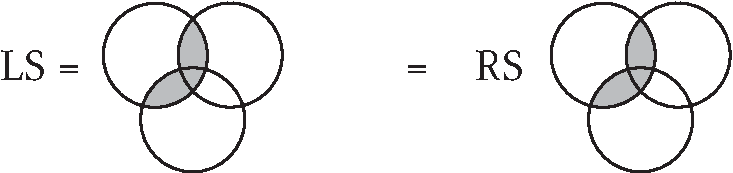
\includegraphics{bilder/kapitel/kap1_Mengen/5.pdf}
\section{Verallgemeinerte Regeln von de Morgan}
\label{sec:VerallgemeinerteRegelnvondeMorgan}
Sind $A_1, A_2 \dots A_n$ alle Teilmengen von $M$ so gilt:
\[\bigcap_{k = 1}^n \overline{A_k} = \bigcup_{k = 1}^n \overline{A_k}\]
\[\bigcup_{k = 1}^n \overline{A_k} = \bigcap_{k = 1}^n \overline{A_k}\]

\section{Aufgaben}
\label{sec:Aufgabe-Mengen-Sportverein}
\subsection{Sportverein}
Von den Mitgliedern eines Sportvereins ist folgendes Bekannt:
\begin{itemize}
	\item Keiner ist zugleich Hand- oder Fu�baller
	\item Alle Eisl�ufer sind Fu�baller
	\item Jeder ist Eisl�ufer oder Skifahrer
\end{itemize}
Zeigen Sie, dass daraus folgt: Jeder Handballspieler ist auch Skifahrer.

L�sung siehe \vref{sec:Loesung-Mengen-Sportverein}.

\subsection{Aufgabe 1}
\label{sec:Aufgabe-Mengen-AufgabeEins}
\renewcommand{\labelenumi}{\alph{enumi})}
\begin{enumerate}
	\item Bestimmen sie $A \backslash B$ und $B \backslash A$ einerseits f�r die Mengen $A=\{1,2,3,4,5\}$ und $B=\{1,2,3\}$ andererseits auch f�r die Mengen $A=\{3,4,5\} $ und $B=\{1,2\}$. Gilt die Aussage $A \backslash B = B \backslash A$? Charakterisieren Sie, wann diese Aussage wahr ist.
	\item Pr�fen Sie die Aussage $A \backslash B = A \cap \overline{B}$ einerseits f�r die Mengen $A=\{1,2,3,4,5\}$ und $B=\{1,2,3\}$, andererseits auch f�r die Mengen $A=\{3,4,5\}$ und $B=\{1,2\}$.
\end{enumerate}

L�sung siehe \vref{sec:Loesung-Mengen-AufgabeEins}.

\subsection{Aufgabe 2}
\label{sec:Aufgabe-Mengen-AufgabeZwei}
Berechnen sie f�r die Teilmenge $D = \{1; 2 ;3 ; \dots; 10\}, S = \{n$ ist Summe zweier Quadrate$\}, P = \{p$ ist Primzahl$\}, U = \{n$ ist ungerade$\}$ und der Grundmenge $\ganzmeng = \{ \dots; -2; -1; 0; 1; 2; \dots \}$ der ganzen Zahlen in die Mengen:
\begin{multicols}{3}
\begin{enumerate}
	\item $P \cap \overline{U}$
	\item $U \cup \overline{U}$
	\item $S \cap D$
	\item $\overline{S} \cap D$
	\item $\left( \overline{S} \cap D \right) \backslash \overline{P}$
	\item $\left( P \cap \overline{U} \right) \times \left( \overline{S} \cap U \right)$
\end{enumerate}
\end{multicols}

L�sung siehe \vref{sec:Loesung-Mengen-AufgabeZwei}.

\chapter{Logik}
Mathematische Inhalte werden durch Aussagen ausgedr�ckt. Eine Aussage beschreibt einen Sachverhalt, der eindeutig entweder wahr $(w)$ oder falsch $(f)$ ist.
Daher:
\begin{enumerate}
\item Au�er wahr und falsch sind keine weiteren Wahrheitswerte zugelassen. (Prinzip vom ausgeschlossenen Dritten)\index{Prinzip vom ausgeschlossenen Dritten}
\item Es trifft genau eine der beiden M�glichkeiten zu. (Prinzip vom ausgeschlossenen Widerspruch)\index{Prinzip vom ausgeschlossenen Widerspruch}
\end{enumerate}
\textalignenum{Beispiel:}{}{
\begin{multicols}{2}[][1em]
\renewcommand{\labelenumi}{\alph{enumi})}
\item $5$ ist kleiner als $3$
\item Bonn ist die Hauptstadt der BRD
\item Gehst du nach Hause?
\item Der einzige Satz ist dieser Zeile ist falsch.
\item Jeder gerade Zahl ist gr��er als $2$ l�sst sich als Summe zweier Primzahlen schreiben.
\item Das Studium der Informatik ist schwer.
\end{multicols}}\\

\textfakealignenum{Beispiel:}{zu }{
\renewcommand{\labelenumi}{zu \alph{enumi})}
\item Aussage mit Wahrheitswert falsch.
\item Aussage mit Wahrheitswert falsch.
\item keine Aussage (da Frage).
\item keine Aussage da man keinen Wahrheitswert zuordnen kann.
\item Aussage mit Wahrheitswert wahr
\item keine Aussage, da objektiv kein bestimmter Wahrheitswert zugeordnet werden kann
\renewcommand{\labelenumi}{\arabic{enumi}.}}

Aus verschiedenen Aussagen werden Definitionen, S�tze und Beweise zusammengesetzt.
\begin{itemize}
\item In einer Definition\index{Definition} wird ein neuer Begriff oder eine Bezeichnung eingef�hrt.\\
		Dieser neue Begriff kann nur durch Beziehungen zu schon vorhandenen Begriffen erkl�rt werden. Dabei st��t man irgendwann auf Grundbegriffe, die sich nicht definieren lassen.
\item In einem Satz\index{Satz} (Theorem)\index{Theorem} wird eine Aussage �ber Eigenschaften von mathematischen Objekten und �ber Beziehungen zwischen Objekten gemacht.\\
		\textalign{Bemerkung:}{Hilfss�tze, Lemmata, Korollare sind auch S�tze.
		\begin{description}
		\item[Hilfssatz] ''kleiner'' eher unwichtiger Satz.\index{Hilfssatz}
		\item[Lemma] ''kleiner'', aber wichtiger Satz.\index{Lemma}
		\item[Korollar] Folgerung aus einem Satz, oft ein wichtiger Spezialfall des Satzes.\index{Korollar}
		\end{description}}
\item Ein Beweis ist ein Nachweis eines Satzes mit Mitteln der Logik.\index{Beweis}
\end{itemize}
Im Folgenden werden Aussagen mit $A, B$ bezeichnet. Diese Zeichen sind Aussagevariablen, die die Werte wahr oder falsch annehmen k�nnen.\\
Zur Definition von Verkn�pfungen und von Aussagen verwendet man Wahrheitstafeln. In einer solchen Tabelle legt man f�r jeder Kombination von Wahrheitswerten fest, welchen Wahrheitswert die Verkn�pfung haben soll.

\section{Definitionen}
\subsection{Verkn�pfung von Aussagen}
\begin{enumerate}
\item Die Negation\index{Negation $\neg$} oder Verneinung\index{Verneinung} der Aussage $A$, ist die Aussage ''nicht $A$'' in Zeichen $ \neg A$ (z.T auch $\overline{A}$), sie ist definiert:\\\\
		%TABL-08.10.2008-mathe-1
		\begin{tabular}{c||c}
		$A$ & $\neg A$\\
		\hline
		$w$ & $f$\\
		$f$ & $w$
		\end{tabular}\\\\
		\textalign{Beispiel:}{\vspace{-0.7em}
		$\begin{array}{rl}
		A & = \mbox{ heute ist Montag}\\
		\neg A & = \mbox{ heute ist nicht Montag}
		\end{array}$}

\item Die Konjunktion\index{Konjunktion $\wedge$} der Aussagen $A$ und $B$, ist die Aussage ''$A$ und $B$'' in Zeichen $A \wedge B$.\\\\
		%TABl-08.10.2008-mathe-2
		\begin{tabular}{c|c||c}
		$A$ & $B$ & $A \wedge B$\\
		\hline
		$w$ & $w$ & $w$\\
		$w$ & $f$ & $f$\\
		$f$ & $w$ & $f$\\
		$f$ & $f$ & $f$
		\end{tabular}\\\\
		$A \wedge B$ ist definiert: $A \wedge B$ ist genau dann richtig, wenn $A$ richtig ist und $B$ richtig ist.\\
		\textalign{Beispiel:}{\vspace{-0.7em}
		$\begin{array}{rl}
		A & = \mbox{ heute ist Montag}\\
		B & = \mbox{ heute ist der Monatsende}\\
		A \wedge B & = \mbox{ heute ist Montag und Monatsende}
		\end{array}$}

\item Die Disjunktion\index{Disjunktion $\vee$} von $A$ und $B$, ist die Aussage ''$A$ oder $B$'' (kein ausschlie�endes oder) in Zeichen $A \vee B$. $A \vee B$ ist definiert:\\\\
		%TABL-08.10.2008-mathe-3
		\begin{tabular}{c|c||c}
		$A$ & $B$ & $A \vee B$\\
		\hline
		$w$ & $w$ & $w$\\
		$w$ & $f$ & $w$\\
		$f$ & $w$ & $w$\\
		$f$ & $f$ & $f$
		\end{tabular}\\\\
		$A \vee B$ ist genau dann falsch, wenn $A$ und $B$ falsch sind.\\
		\textalign{Beispiel:}{
		$A, B $ wie oben\\
		$A \vee B $ heute ist Montag oder heute ist Monatsende (oder heute ist Montag und Monatsende)}

\item Die Implikation\index{Implikation $\Rightarrow$} von $A$ nach $B$ ist die Aussage ''wenn $A$ dann $B$'' oder ''aus $A$ folgt $B$'', in Zeichen $A \Rightarrow B$.\\$A \Rightarrow B$ ist definiert durch:\\\\
		%TABL-08.10.2008-4
		\begin{tabular}{c|c||c}
		$A$ & $B$ & $A \Rightarrow B$\\
		\hline
		$w$ & $w$ & $w$\\
		$w$ & $f$ & $f$\\
		$f$ & $w$ & $w$\\
		$f$ & $f$ & $w$
		\end{tabular}\\\\
		Die Aussage $A \Rightarrow B$ ist genau dann falsch, wenn $B$ falsch und $A$ richtig ist.\\
		Man nennt $A$ die Voraussetzung und $B$ die (Schluss)Folgerung.\\
		Man sagt auch $A$ ist eine hinreichend Bedingung f�r $B$ beziehungsweise $B$ ist eine notwendige Bedingung f�r $A$.\\
		\textalignenum{Beispiel:}{}{
		\item $A = $ es regnet\\
				$B = $ die Stra�e ist nass
		\item $A = $ Karlsruhe liegt in Bayern\\
				$B = 1+1 = 3$}

\item Die �quivalenz\index{�quivalenz $\Leftrightarrow$} von $A$ und $B$ ist die Aussage ''$A$ gilt genau dann wenn $B$ gilt'' beziehungsweise ''$A$ gilt dann und nur dann wenn $B$ gilt'', in Zeichen $A \Leftrightarrow B$ (''$A$ ist �quivalent zu $B$''). $A \Leftrightarrow B$ ist definiert durch:\\\\
		%TABL-08.10.2008-mathe-5
		\begin{tabular}{c|c||c}
		$A$ & $B$ & $A \Leftrightarrow B$\\
		\hline
		$w$ & $w$ & $w$\\
		$w$ & $f$ & $f$\\
		$f$ & $w$ & $w$\\
		$f$ & $f$ & $w$
		\end{tabular}\\\\
		$A \Leftrightarrow B$ ist gleichwertig zu $(A \Rightarrow B) \wedge (B \Rightarrow A)$\\\\
		%TABL-08.10.2008-mathe-6
		\begin{tabular}{c|c||c|c|c}
		$A$ & $B$ & $A \Rightarrow B$ & $B \Rightarrow A$ & $(A \Rightarrow B) \wedge (B \Rightarrow A)$\\
		\hline
		$w$ & $w$ & $w$ & $w$ & $w$\\
		$w$ & $f$ & $f$ & $w$ & $f$\\
		$f$ & $w$ & $w$ & $f$ & $f$\\
		$f$ & $f$ & $w$ & $w$ & $w$
		\end{tabular}\\\\
		da die ''Inputspalten'' links und die ''Outputspalten'' rechts der letzten beiden Tabellen �bereinstimmen ist $A \Leftrightarrow B$ gleichbedeutend mit $(A \Rightarrow B) \wedge (B \Rightarrow A)$\\
		\textalign{Beispiel:}{
		$A = x$ ist durch $2$ teilbar\\
		$B = x$ ist eine gerade Zahl\\
		$A \Leftrightarrow B$, da entweder $A$ und $B$ richtig oder $A$ und $B$ falsch sind}
\end{enumerate}
\subsection{Tautologie und Kontradiktion}
\renewcommand{\labelenumi}{\arabic{enumi}.}
\begin{enumerate}
	\item Eine Aussage, die immer wahr ist hei�t Tautologie\index{Tautologie}.
	\item Eine Aussage, die immer falsch ist nennt man Kontradiktion\index{Kontradiktion}.
\end{enumerate}
\textalignenum{Beispiel:}{zu }{
\renewcommand{\labelenumi}{zu \arabic{enumi}.}
\item $A \vee \neg A$ (Gesetz des ausgeschlossenen Dritten)\index{Gesetz des ausgeschlossenen Dritten}
\item $A \Leftrightarrow \neg (\neg A)$ (Gesetz der doppelten Verneinung)\index{Gesetz der doppelten Verneinung}
\renewcommand{\labelenumi}{\arabic{enumi}.}}

\subsection{Allquantor und Existenzquantor}
\begin{enumerate}
\item Gilt eine Aussage $A(x)$ f�r alle $x$, so schreibt man
		\[\forall x: A(x) \mbox{ (f�r alle $x$ gilt die Aussage $A(x)$)}\]
		\[\forall \mbox{ hei�t Allquantor}\]\index{Allquantor}

\item Gilt eine Aussage $A(x)$ f�r mindestens ein $x$, so schreibt man
		\[\exists x: A(x) \mbox{ (es existiert mindestens ein $x$ f�r das die Aussage $A(x)$ gilt)}\]
		\[\exists \mbox{ hei�t Existenzquantor}\]\index{Existenzquantor}

\item Wenn die Aussage $A(x)$ f�r genau ein $x$ gilt, schreibt man
		\begin{alignat*}{2}
			&\exists^1 &&x: A(x) \mbox{ (es gibt genau ein $x$ mit der Eigenschaft $A(x)$}\\
			&\exists^{=1} &&x: A(x)\\
			&\exists! &&x: A(x)\\
			&\exists_1 &&x: A(x)
		\end{alignat*}

\item Wenn die Aussage $A(x)$ f�r genau $n$ verschiedene $x$ Werte gilt, schreibt man
		\[\exists^{=n} x: A(x)\]
\end{enumerate}
\textalignenum{Beispiel:}{zu }{
\renewcommand{\labelenumi}{zu \arabic{enumi}.}
\item $\forall x: x^2 \geq 0$ (genauer $\forall x \in \relmeng: x^2 \geq 0$)
\item $\exists x \in \mathbb{P}: x$ gerade ($\mathbb{P} =$ Menge der Primzahlen)
\item $\exists! x \in \mathbb{P}: x$ gerade
\renewcommand{\labelenumi}{\arabic{enumi}.}}

\textalign{Bemerkung:}{
\begin{itemize}[leftmargin=1.28em]
\item Die Aussage $\forall x \in \mathbb{X}: A(x)$ entspricht der Aussage $\bigwedge_{x \in \mathbb{X}} A(x)$, also der Konjunktion aller $A(x)$
\item Die Aussage $\exists x \in \mathbb{X}: A(x)$, entspricht der Aussage $\bigvee_{x \in \mathbb{X}} A(x)$, also der Disjunktion aller $A(x)$
\end{itemize}}

\subsection{Verneinung der Quantoren}
\label{Satz_Verneinung_der_Quantoren}
\begin{enumerate}
\item $\neg (\forall x: A(x)) \aeq \exists x: \neg A(x)$
\item $\neg (\exists x: A(x)) \aeq \forall x: \neg A(x)$
\end{enumerate}
Beweis: -\\
\textalign{Bemerkung:}{Satz \vref{Satz_Verneinung_der_Quantoren} entspricht der Verallgemeinerung der Regeln von de Morgan auf allgemeine Indexmengen $\RM{1}$\\
\[\neg \left(\forall x \in \RM{1}: A(x)\right) \aeq \neg \left(\bigwedge_{x \in \RM{1}} A(x)\right) \aeq \bigvee_{x \in \RM{1}} \left(\neg A(x)\right) \aeq \exists x \in \RM{1}: \neg A(x)\]}

\textalign{Beispiel:}{
$M$ Mengen aller Musiker eines Orchesters\\
$A(m) = $ Musiker $m$ spielt falsch\\
$\forall m \in M: A(m)$ Alle Musiker spielen falsch\\
$\neg (\forall m \in M: A(m))$ mindestens ein Musiker spielt richtig\\
$\exists m \in M: A(m)$ mindestens ein Musiker spielt falsch\\
$\neg (\exists m \in M: A(m))$ alle Musiker spielen richtig}

\subsection{\texorpdfstring{Beweisstrategien f�r S�tze der Form $A \Ra B$}{Beweisstrategien f�r S�tze der Form A dann B}}
\begin{enumerate}
\item Direkter Beweis\index{Direkter Beweis}\\\\
		\begin{tabular}{c|c||c}
			$A$ & $B$ & $A \Ra B$
			\\\hline
			$w$ & $w$ & $w$
			\\$w$ & $f$ & $f$
			\\$f$ & $w$ & $w$
			\\$f$ & $f$ & $w$
		\end{tabular}\\\\
		Man nimmt an $A$ ist wahr und folgert daraus, dass $B$ wahr ist (d.h Fall $A$ wahr, $B$ falsch tritt nicht auf)\\
		\textalign{Beispiel:}{
		\textalign{Behauptung:}{
		\textfakealign{$\Ra$}{}{$\overbrace{x \mbox { durch } 4 \mbox { teilbar}}^{A(x)}$}\\
		\textalign{$\Ra$}{$\underbrace{x \mbox { durch } 2 \mbox { teilbar}}_{B(x)}$}}}\\
		\textfakealign{Beispiel:}{}{
		Sei $A(x)$ wahr\\$x$ durch $4$ teilbar
		\begin{alignat*}{2}
			&\aeq \frac{x}{4} = c~&&c \in \mathbb{Z}\\
			&\aeq \frac{x}{2} = 2c~&&c \in \mathbb{Z}\\
			&\aeq \frac{x}{2} = d~&&d \in \mathbb{Z}\\
			&\aeq x \mbox{ ist durch $2$ teilbar}\\
			&\aeq B(x) \mbox{ ist wahr}\
		\end{alignat*}}

\item Kontraposition\index{Kontraposition} ($\Ra$ indirekter Beweis\index{Indirekter Beweis})\\\\
		\begin{tabular}{c|c||c|c}
			$A$ & $B$ & $A \Ra B$ & $\neg B \Ra \neg A$
			\\\hline
			$w$ & $w$ & $w$ & $w$
			\\$w$ & $f$ & $f$ & $f$
			\\$f$ & $w$ & $w$ & $w$
			\\$f$ & $f$ & $w$ & $w$
		\end{tabular}\\\\
		Wegen der �quivalenz der Aussagen $A \Ra B$ und $\neg B \Ra \neg A$ k�nnen wir die zweite statt der ersten zeigen\\
		Wir nehmen an $B$ sei falsch und folgen daraus, $A$ ist falsch (damit tritt der Fall $A$ wahr, $B$ falsch nicht auf)\\
		\textalign{Beispiel:}{\textalign{Behauptung:}{$\underbrace{n^2 \mbox{ gerade}}_{A(n)} \Ra \underbrace{n \mbox{ gerade}}_{B(n)} (n \in \mathbb{N})$}}\\
		\textfakealign{Beispiel:}{}{\textalign{Beweis:}{
		Wir nehmen an $B(n)$ ist falsch, daher $n$ ist ungerade
		\begin{alignat*}{2}
			 \aeq n 	&= 2 m + 1~~m \in \mathbb{N}\\
			 \Ra n^2 &= (2m + 1)^2 = (2m)^2 + 2(2m) \mal 1 + 1^2\\
						&= \underbrace{\underbrace{4 m^2}_{\mbox{gerade}} + \underbrace{4m}_{\mbox{gerade}} +1}_{\mbox{ungerade}}\\
			&\aeq A(n) \mbox{ ist falsch}
		\end{alignat*}}}

\item Wiederspruchsbeweis\index{Wiederspruchsbeweis} ($\Ra$ indirekter Beweis\index{Indirekter Beweis})\\\\
		\begin{tabular}{c|c||c}
			$A$ & $B$ & $A \Ra B$
			\\\hline
			$w$ & $w$ & $w$
			\\$w$ & $f$ & $f$
			\\$f$ & $w$ & $w$
			\\$f$ & $f$ & $w$
		\end{tabular}\\\\
		Man nimmt an $A$ sei wahr und $B$ sei falsch($\equals$ einziger Fall indem $A \Ra B$ falsch ist) und zeigt, dass diese Annahmen zu einem Widerspruch f�hren.\\
		\textalign{Beispiel:}{\textalign{Behauptung:}{$\sqrt{2}$ ist irrational (also nicht in $\mathbb{Q}$)
		$\aeq \underbrace{x^2 = 2}_{A(x)} \Ra \underbrace{x \mbox{ ist irrational}}_{B(x)}$}}
		\textfakealign{Beispiel:}{}{\textalign{Beweis:}{Wir nehmen an
		\begin{align*}
				   x^2 &= 2 \mbox{ und } x \mbox{ rational}\\
		    \aeq x^2 &= 2 \mbox{ und es existiert $p,q$ teilerfremd } x = \frac{p}{q}\\
			 \sqrt{2} &= x =\frac{p}{q}\\
						 &\Ra 2 = x^2 = \frac{p^2}{q^2}\\
				  		 &\aeq \underbrace{2q^2}_{\mbox{gerade}} = \underbrace{p^2}_{\mbox{gerade}} \mbox{ (*)}\\
						 &\Ra p \mbox{ gerade } \Ra p = 2m~~m \in \mathbb{Z}\\
						 &\Ra p^2 = (2m)^2 = 4 m^2
		\end{align*}
		\begin{align*}
			\mbox{in (*)} &2 q^2 = 4 m^2\\
			\aeq &q^2 = \underbrace{2m^2}_{\mbox{gerade}}\\
			&\Ra q \mbox{ gerade } \lightning p,q \mbox{ sollen teilfremd sein}
		\end{align*}}}
\end{enumerate}
\textalign{Bemerkung:}{S�tze der Form $A \aeq B$ zerlegt man f�r den Beweis normalerweise und zeigt $A \Ra B$ und $B \Ra A$.}

\section{\texorpdfstring{Rechenregeln f�r $\wedge, \vee, \neg, \Rightarrow,$ und $\Leftrightarrow$}{Rechenregeln f�r Logik Verkn�pfungen}}
\label{sec_Rechenregeln_f�r_Logikverkn�pfungen}
\subsection{Assoziativgesetz}
\index{Logik!Assoziativgesetz}
\begin{enumerate}
	\item $(A \wedge B) \wedge C \Longleftrightarrow A \wedge (B \wedge C)$
	\item $(A \vee B) \vee C \Longleftrightarrow A \vee (B \vee C)$
	\item $(A \Leftrightarrow B) \Leftrightarrow C \Longleftrightarrow A \Leftrightarrow (B \Leftrightarrow C)$
\end{enumerate}

\subsection{Kommutativgesetz}
\index{Logik!Kommutativgesetz}
\begin{enumerate}
	\item $A \wedge B \Longleftrightarrow B \wedge A$
	\item $A \vee B \Longleftrightarrow B \vee A$
	\item $A \Leftrightarrow B \Longleftrightarrow B \Leftrightarrow A$
\end{enumerate}

\subsection{Distributivgesetz}
\index{Logik!Distributivgesetz}
\begin{enumerate}
	\item $A \wedge (B \vee C) \Longleftrightarrow (A \wedge B) \vee (A \wedge C)$
	\item $A \vee (B \wedge C) \Longleftrightarrow (A \vee B) \wedge (A \vee C)$
\end{enumerate}

\subsection{Idempotenzgesetz}
\index{Logik!Idempotenzgesetz}
\begin{enumerate}
	\item $A \wedge A \Longleftrightarrow A$
	\item $A \vee A \Longleftrightarrow A$
\end{enumerate}

\subsection{Absorptionsgesetz}
\index{Logik!Absorptionsgesetz}
\begin{enumerate}
	\item $A \wedge (B \vee A) \Longleftrightarrow A$
	\item $A \vee (B \wedge A) \Longleftrightarrow A$
\end{enumerate}

\subsection{Gesetz von de Morgan}
\index{Logik!Gesetz von de Morgan}
\begin{enumerate}
	\item $\neg (A \wedge B) \Longleftrightarrow \neg A \vee \neg B$
	\item $\neg (A \vee B) \Longleftrightarrow \neg A \wedge \neg B$
\end{enumerate}

\subsection{Kontraposition}
\index{Logik!Kontraposition}
\[A \Rightarrow B \Longleftrightarrow \neg B \Rightarrow \neg A\]
\textalign{Beweis:}{�ber Wahrheitstafeln, Assoziativgesetz\\\\
\begin{tabular}{c|c|c||c|c||c|c||c}
$A$ & $B$ & $C$ & $A \Leftrightarrow B$ & $(A \Leftrightarrow B) \Leftrightarrow C$ & $B \Leftrightarrow C$ & $A \Leftrightarrow (B \Leftrightarrow C)$ & $D \Leftrightarrow E$\\
\hline
$w$ & $w$ & $w$ & $w$ & $w$ & $w$ & $w$ & $w$\\
$w$ & $w$ & $f$ & $w$ & $f$ & $f$ & $f$ & $w$\\
$w$ & $f$ & $w$ & $f$ & $f$ & $f$ & $f$ & $w$\\
$w$ & $f$ & $f$ & $f$ & $w$ & $w$ & $w$ & $w$\\
\hline
$f$ & $w$ & $w$ & $f$ & $f$ & $w$ & $f$ & $w$\\
$f$ & $w$ & $f$ & $f$ & $w$ & $f$ & $w$ & $w$\\
$f$ & $f$ & $w$ & $w$ & $w$ & $f$ & $w$ & $w$\\
$f$ & $f$ & $f$ & $w$ & $f$ & $w$ & $f$ & $w$
\end{tabular}}

\textalign{Beweis:}{Kontraposition\\
$ A \Rightarrow B \Longleftrightarrow \neg B \Rightarrow \neg A$\\
\begin{tabular}{c|c||c||c|c|c||c|c}
$A$ & $B$ & $A \Rightarrow B$ & $\neg B$ & $\neg A$ & $\neg B \Rightarrow \neg A$ & $(A \Rightarrow B) \Leftrightarrow (\neg B \Rightarrow \neg A)$\\
\hline
$w$ & $w$ & $w$ & $f$ & $f$ & $w$ & $w$\\
$w$ & $f$ & $f$ & $w$ & $f$ & $f$ & $w$\\
$f$ & $w$ & $w$ & $f$ & $w$ & $w$ & $w$\\
$f$ & $f$ & $w$ & $w$ & $w$ & $w$ & $w$
\end{tabular}}

\textalign{Bemerkung:}{Alle Aussagen des Satzes \vref{sec_Rechenregeln_f�r_Logikverkn�pfungen} sind Tautologien.}

\section{Aufgaben}
\begin{tabular}{c|c||c}
$A$ & $B$ & $A \Rightarrow B$\\
\hline
$w$ & $w$ & $w$\\
w & f & f\\
f & w & f\\
f & f & w
\end{tabular}

\renewcommand{\labelenumi}{\arabic{enumi}.}
\begin{enumerate}
	\item $A = x$ ist durch 2 teilbar\\$B = x$ eine gerade Zahl\\$B$ und $A$ sind beide wahr oder beide falsch $A \Leftrightarrow B$ wahr (daher $A$ und $B$ sind �quivalent)
	\item $A = x$ ist durch 2 teilbar\\$B = x$ ist ungerade\\damit ist immer genau eine der beiden Aussagen richtig und die andere falsch $A \Leftrightarrow B$ falsch ($A$ und $B$ sind nicht �quivalent)
	\item $A = x$ ist durch 2 teilbar\\$B = x$ ist durch 4 teilbar\\daher $A \Leftrightarrow B$ kann wahr oder falsch sein ($A$ und $B$ sind keine �quivalenten Aussagen)
	\item $A = 1 + 1 = 3$\\$B = $ Regensburg liegt im Saarland\\Da beide Aussagen falsch sind gilt $A \Leftrightarrow B$ (also insbesondere da $1 + 1 = 3$ folgt ''Regensburg liegt im Saarland'')
\end{enumerate}
\textalign{Bemerkung:}{
\begin{itemize}[leftmargin=1.28em]
	\item Zwei immer wahre Aussagen sind �quivalent
	\item Zwei immer falsche Aussagen sind �quivalent
\end{itemize}}

\subsection{Aufgabe 1.2}
\label{sec:Aufgabe-Logik-AufgabeEinsPunktZwei}
Es seien $A$ und $B$ zwei Aussagen. Bestimmen sie die Wahrheitswerte der Aussagen
\renewcommand{\labelenumi}{\alph{enumi})}
\begin{enumerate}
	\item $(A \vee B) \wedge \neg A$
	\item $(A \wedge B) \vee \neg A$
	\item $(\neg A \wedge \neg B) \vee A$
\end{enumerate}

L�sung siehe \vref{sec:Loesung-Logik-AufgabeEinsPunktZwei}.

\subsection{Aufgabe 1.3}
\label{sec:Aufgabe-Logik-AufgabeEinsPunktDrei}
Sind die folgenden Aussagen richtig oder falsch?
\renewcommand{\labelenumi}{\alph{enumi})}
\begin{enumerate}
	\item Wenn $18$ durch $12$ teilbar ist, dann ist 18 durch 3 teilbar.
	\item $3$ ist genau dann Teiler von $8$, wenn $14$ eine Primzahl ist.
\end{enumerate}

L�sung siehe \vref{sec:Loesung-Logik-AufgabeEinsPunktDrei}.

\subsection{Aufgabe 6}
\label{sec:Aufgabe-Logik-AufgabeSechs}
Es seien $A, B$ Aussagen. Bestimmen sie die Wahrheitstafel der folgenden Formeln
\renewcommand{\labelenumi}{\alph{enumi})}
\begin{enumerate}
\item $(\neg (A \und B)) \und ((\neg A) \oder B)$
\item $((\neg A) \oder B) \Ra (A \und B)$
\end{enumerate}
\renewcommand{\labelenumi}{\arabic{enumi}.}

L�sung siehe \vref{sec:Loesung-Logik-AufgabeSechs}.

\subsection{Aufgabe 7}
\label{sec:Aufgabe-Logik-AufgabeSieben}
Es seien $A, B, C$ Aussagen. Zeigen sie mit Hilfe einer Wahrheitstafel die �quivalenz der Formeln
\renewcommand{\labelenumi}{\alph{enumi})}
\begin{enumerate}
\item $(A \oder B) \Ra \neg C$
\item $C \Ra (\neg A) \und (\neg B)$
\end{enumerate}
\renewcommand{\labelenumi}{\arabic{enumi}.}

L�sung siehe \vref{sec:Loesung-Logik-AufgabeSieben}.

\subsection{Aufgabe 8}
\label{sec:Aufgabe-Logik-AufgabeAcht}
Dr�cken sie $F_1, F_2, F_3$ mithilfe von $A, B, \und, \oder, \neg$ aus.\\\\
\begin{tabular}{c|c||c|c|c}
	$A$ & $B$ & $F_1$ & $F_2$ & $F_3$
	\\\hline
	$w$ & $w$ & $f$ & $f$ & $w$
	\\$w$ & $f$ & $f$ & $w$ & $f$
	\\$f$ & $w$ & $w$ & $f$ & $f$
	\\$f$ & $f$ & $f$ & $f$ & $w$
\end{tabular}

L�sung siehe \vref{sec:Loesung-Logik-AufgabeAcht}.

\subsection{Aufgabe 9}
\label{sec:Aufgabe-Logik-AufgabeNeun}
Tragen sie in die unten stehende unvollst�ndige Wahrheitstafel die fehlende Wahrheitswerte ein.\\\\
\begin{tabular}{c|c|c|c||c|c|c}
$A$ & $B$ & $C$ & $D$ & $(A \oder B) \und D$ & $\overline{(A \oder B)} \und (C \oder D)$ & $C \Ra ((A \und D) \oder (B \und D))$
\\\hline
$f$ & \textvisiblespace & $f$ & \textvisiblespace & $w$ & \textvisiblespace & \textvisiblespace\\
$w$ &    $w$ & \textvisiblespace & \textvisiblespace & \textvisiblespace & \textvisiblespace & $f$\\
\textvisiblespace & \textvisiblespace & $f$ & \textvisiblespace & \textvisiblespace & $w$ & \textvisiblespace
\end{tabular}

L�sung siehe \vref{sec:Loesung-Logik-AufgabeNeun}.

\subsection{Aufgabe 10}
\label{sec:Aufgabe-Logik-AufgabeZehn}
Verneinen sie die Aussagen:
\renewcommand{\labelenumi}{\alph{enumi})}
\begin{enumerate}
\item Alle Quadratzahlen sind gerade.
\item Es gibt nat�rliche Zahlen die nicht rational sind.
\item Alle Stra�en und mindestens ein Pfad f�hren nach Rom.
\end{enumerate}
\renewcommand{\labelenumi}{\arabic{enumi}.}

L�sung siehe \vref{sec:Loesung-Logik-AufgabeZehn}.

\chapter{Relation und Abbildungen}
\section{Darstellung von Relationen}
$A, B$ endliche Mengen
\begin{enumerate}
\item In Worten: $xRy \equals$ ''$x$ steht in Relation zu $y$''
\item Als Menge geordneter Paare
		\begin{itemize}
		\item Aufz�hlung
		\item Graphische Darstellung
		\end{itemize}
\item Als gerichteten Graphen\\
		Die Elemente von $A$ beziehungsweise $B$ werden als Knoten aufgefasst. Gilt $(x, y) \in \relmeng$ wird eine gerichtete Kante (Pfeil) vom Koten $x \in A$ zum Knoten $y \in B$ gezeichnet.
\item Als Matrix\\
		Zuerst werden die Elemente der Mengen $A$ und $B$ durchnummeriert.\\
		$A = $\gklamm{x_1, x_2, \dots, x_n}, B = \gklamm{y_1, y_2, \dots, y_m}\\
		Dann kann man die Wahrheitswerte
		\[M(i, j) = \left\{\begin{array}{c}w \mbox{ falls } (x_i, y_j) \in R\\f \mbox{ falls } (x_i, y_j) \in R \end{array}\right.\]
		\[i \in \gklamm{1, 2, \dots, n}, j \in \gklamm{1, 2, \dots, m}\]
		definiert. Diese Werte kann man eine $n \times m$ Matrix eintragen: ($n$ Zeilen, $m$ Spalten)
		\[\left(\begin{array}{cccc}
		M(1, 1) & M(1, 2) & \dots 	& M(1, m)\\
		M(2, 1) & \dots	& \dots	&\vdots\\
		M(n, 1) & \dots	& \dots	&M(n, m)
		\end{array}\right)\]
\end{enumerate}
\textalignenum{Beispiel:}{zu }{
\renewcommand{\labelenumi}{zu \arabic{enumi})}
\item $R$ definiert durch $x$ sei $\geqq y$ mit $x \in A = $\gklamm{1, 2, 3}, $y \in B$ = \gklamm{0, 2, 4, 6}
\item $R = $\gklamm{(1,0), (3,2), (3,0), (2,0), (2,2)}\\
		%TAB-15.10.2008-math-1
		
\includegraphics{bilder/kapitel/kap3_Relation_und_Abbildungen/1.pdf}

\item $ $\newline %TODO -- Fix the top/bottom/middle problem
		%TAB-15.10.2008-math-2
		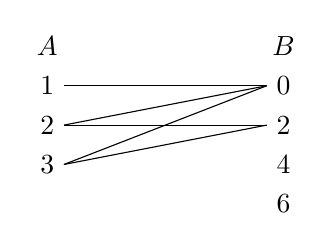
\begin{tikzpicture}
		%Nodes
		\node (Left_Over) 	at (0,0.5) 		{$A$};
		\node (Left_1) 		at (0,0) 		{$1$};
		\node (Left_2) 		at (0,-0.5) 	{$2$};
		\node (Left_3) 		at (0,-1) 		{$3$};
		\node (Right_Over) 	at (3,0.5) 		{$B$};
		\node (Right_1) 		at (3,0) 		{$0$};
		\node (Right_2) 		at (3,-0.5) 	{$2$};
		\node (Right_3) 		at (3,-1) 		{$4$};
		\node (Right_4) 		at (3,-1.5) 	{$6$};
		%Verkn�pfungen
		\draw (Left_1.east) -- (Right_1.west);
		\draw (Left_2.east) -- (Right_1.west);
		\draw (Left_2.east) -- (Right_2.west);
		\draw (Left_3.east) -- (Right_1.west);
		\draw (Left_3.east) -- (Right_2.west);
		\end{tikzpicture}

\item $A = $\gklamm{1 (x_1), 2 (x_2), 3 (x_3)} $B = $\gklamm{0 (y_1), 2 (y_2), 4 (y_3), 6 (y_4)}\\
		\[\left(\begin{array}{cccc}
		w & f & f & f\\
		w & w & f & f\\
		w & w & f & f
		\end{array}\right)\]

		Bemerkung: Relation wie oben mit $B = A = $\gklamm{1, 2, 3}

		\textalign{Darstellung 3:}{$ $\newline %TODO -- Fix the top/bottom/middle problem
		%TAB-15.10.2008-math-3
		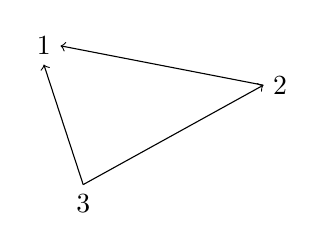
\begin{tikzpicture}
		%Nodes
		\node (Eins) at (0,0) 		{$1$};
		\node (Zwei) at (3,-0.5) 		{$2$};
		\node (Drei) at (0.5,-2)	{$3$};
		%Verkn�pfungen
		\draw[->] (Zwei.west)	-- (Eins.east);
		\draw[->] (Drei.north) 	-- (Eins.south);
		\draw[->] (Drei.north) 	-- (Zwei.west);
		\end{tikzpicture}}
\renewcommand{\labelenumi}{\arabic{enumi}.}}

\section{Definitionen}
\subsection{Relation}
Seien $A$ und $B$ Mengen und $R \subseteq A \times B$, dann hei�t $R$ Relation auf $A \times B$.\\
Ist $B = A$, so hei�t $R$ Relation auf $A$.\\
Eine Relation definiert eine Beziehung, die zwischen den Komponenten der Paare $(x, y) \in A \times B$ besteht. Dabei l�sst sich f�r jedes dieser Paare $(x, y)$ festlegen, ob die gegebene Beziehung wahr oder falsch ist.\\
Besteht zwischen $x$ und $y$ die durch $R$ definierte Relation, so schreibt man $(x, y) \in R$ h�ufig $xRy$.

\subsection{Spezielle Relationen}
Sei $R$ eine Relation auf der nichtleeren Menge $A$. Die Relation $A$ hei�t:
\begin{enumerate}
\item reflexiv: wenn f�r alle $x \in A$ gilt: \[xRx\]
\item symmetrisch: wenn f�r alle $x, y \in A$ gilt: \[xRy \Ra yRx\]
\item antisymmetrisch: wenn f�r alle $x, y \in A$ gilt: \[(xRy \und yRx) \Ra x = y\]
\item transitiv: wenn f�r alle $x, y, z \in A$ gilt: \[xRy \und yRz \Ra xRz\]
\item vollst�ndig: wenn f�r alle $(x, y) \in A \times A$ gilt:\[xRy \oder yRx\]
\end{enumerate}
\textalign{Beispiel:}{
Die Produktion einer Maschine erfordert 6 Produktionsschritte. Zuerst muss 1 ausgef�hrt werden, dann die Schritte 2, 3, 4 in beliebiger Reihenfolge und dann 5, 6 in beliebiger Reihenfolge
\begin{align*}
	A_1 &= \gklamm{1, 2, 3, 4, 5, 6}\\
	R_1 &= \gklamm{(x, y) \in A_1 \times A_1 | y \mbox{ kann nicht vor } x \mbox{ ausgef�hrt werden}}\\
	R   &= \left\{(1,2), (1,3), (1,4), (1,5), (1,6), (2,5), (2,6), (3,5), (3,6),\right.\\
		 &\left.(4,5), (4,6), (1,1), (2,2), (3,3), (4,4), (5,5), (6,6)\right\}
\end{align*}
\begin{tabular}{r|c|c}
& \begin{sideways}wahr\end{sideways} & \begin{sideways}falsch\end{sideways}\\
\hline
reflexiv				& x 	&\\
\hline
symmetrisch 		& 		& x\\
\hline
antisymmetrisch 	& x 	&\\
\hline
transitiv 			& x 	&\\
\hline
vollst�ndig 		&  	& x
\end{tabular}}
\subsection{�quivalenzrelation}
Eine Relation auf $A$ nennen wir dann �quivalenzrelation, wenn sie reflexiv, transitiv und symmetrisch ist.\\
Im Fall einer �quivalenzrelation schreibt man meist $x \thicksim y$ anstelle von $xRy$ oder $(x,y) \in R$ ($x \thicksim y \equals$ ''$x$ ist �quivalent zu $y$'')

\subsection{�quivalenzklasse}
Ist $A$ eine nichtleere Menge und $R \subseteq A \times A$ eine �quivalenzrelation auf $A$, so hei�t f�r ein Element $a \in A$ die Menge
\[[a] = \gklamm{x \in A \vert x \thicksim a} = \gklamm{x \in A \vert a \thicksim x}\]
die �quivalenzklasse von a.\\
Wegen der Reflexivit�t folgt $a \in [a]$ f�r jedes $a \in A$.
Beispiel:\\
\begin{minipage}{10mm}
\LARGE R = \normalsize
\end{minipage}
\begin{minipage}{40mm}
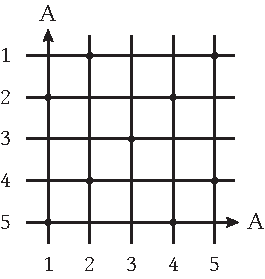
\includegraphics{bilder/kapitel/kap3_Relation_und_Abbildungen/5.pdf}
\end{minipage}\\
bereits gezeigt $R$ reflexiv, transitiv, symmetrisch,\\
$\Ra$ �quivalenzrelation\\
\[\left.
\begin{array}{l}
\lbrack 1 \rbrack = \{1, 4\}\\
\lbrack 2 \rbrack = \{2, 5\}\\
\lbrack 3 \rbrack = \{3	\}\\
\lbrack 4 \rbrack = \{4, 1\}\\
\lbrack 5 \rbrack = \{5, 2\}
\end{array}
\right\}
\begin{array}{l}
\lbrack 1 \rbrack = \lbrack 4 \rbrack = \{1, 4\}\\
\lbrack 2 \rbrack = \lbrack 5 \rbrack = \{2, 5\}\\
\lbrack 3 \rbrack = \{3\}
\end{array}\]
$[1] \cup [2] \cup [3] = \{1, 2, 3, 4, 5\}$
\begin{alignat*}{2}
	&[1] \cap [2] = \emptyset\\
	&[1] \cap [3] = \emptyset\\
	&[2] \cap [3] = \emptyset\\
\end{alignat*}
\subsection{Ordnungsrelation}
Sei $A$ eine nichtleere Menge
\begin{enumerate}
\item Eine Relation auf $A$ nennt man Ordnungsrelation auf $A$, falls sie reflexiv, transitiv und antisymmetrisch ist. In diesem Fall schreibt man meistens $a \leq b$ anstatt $aRb$ oder $(a, b) \in R$
\item Eine Ordnungsrelation $R$ auf $A$ hei�t vollst�ndig oder Totalordnung, falls sie vollst�ndig ist.
\end{enumerate}
\subsection{Funktion und Abbildung}
Seien $D$ und $B$ zwei nichtleere Mengen. Dann hei�t die Menge $f \subseteq D \times B$ eine Funktion oder Abbildung von $D$ nach $B$, falls gilt:
\[\forall x \in D~~\exists ! y \in B~~(x, y) \in f\]
\subsubsection{Schreibweisen und Bezeichnungen}
\begin{itemize}
\item $f: D \rightarrow B \Longleftrightarrow f \subseteq D \times B$
\item $y = f(x) \Longleftrightarrow x \mapsto y \Longleftrightarrow (x,y) \in f$
\item $D$ hei�t Definitionsbereich von $f$
\item $f(x)$ hei�t Bild von $x \in D$ unter $f$
\item $f [D] := \gklamm{f(x) \in D} = \bigcup_{x \in D} \gklamm{f(x)}$ hei�t Bildmenge von $f^{x \in D}$
\item $B$ hei�t Wertebereich von $f$
\item f�r $T \subseteq B$ hei�t $f^{-1} [T] = \gklamm{x \in D \vert f(x) \in T}$ die Urbildmenge von $T$ unter $f$.
\end{itemize}
\textalignenum{Beispiel:}{}{
\item $f \mathbb{Z} \rightarrow \mathbb{N}$\\
		$x \mapsto x^2 + 1$\\
		$x \in \mathbb{Z}, x^2 \in \mathbb{Z}$\\\\
		\begin{tabular}{ll}
		Definitionsbereich & $D = \mathbb{Z}$\\
		Wertebereich & $B = \mathbb{N}$\\
		Bildmenge & $f [D] \supseteq \gklamm{1, 2, 5, 10, \dots}$
		\end{tabular}\\\\
		schwer anzugeben, deshalb verwendet man einen Wertebereich, der $f [D]$ enth�lt $(f [D] \subseteq B)$\\
		$T = \gklamm{2, 3, 4, 5, 6, 7, 8, 9, \dots, 20}$\\
		$f^{-1} [T] = \gklamm{\pm 1, \pm 2, \pm 3, \pm 4}$

\item Sei $D = B := \gklamm{1, 2, 3, 4, 5}$, die Abbildung $f D \rightarrow B$ sei definiert durch\\
		\begin{minipage}{50mm}
		\begin{align*}
			1 \mapsto f (1) &= 1\\
			2 \mapsto f (2) &= 1\\
			3 \mapsto f (3) &= 3\\
			4 \mapsto f (4) &= 4\\
			5 \mapsto f (5) &= 4
		\end{align*}
		\end{minipage}
		\begin{minipage}{50mm}
		%IMG-23.10.2008-mathe-1
		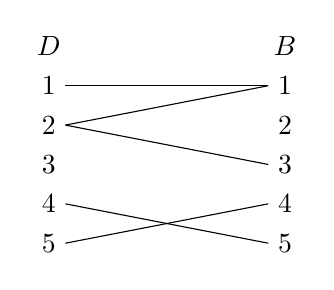
\begin{tikzpicture}
		%Nodes
		\node (Left_Over) 	at (0,0.5) 		{$D$};
		\node (Left_1) 		at (0,0) 		{$1$};
		\node (Left_2) 		at (0,-0.5) 	{$2$};
		\node (Left_3) 		at (0,-1) 		{$3$};
		\node (Left_4) 		at (0,-1.5) 	{$4$};
		\node (Left_5) 		at (0,-2) 		{$5$};
		\node (Right_Over) 	at (3,0.5) 		{$B$};
		\node (Right_1) 		at (3,0) 		{$1$};
		\node (Right_2) 		at (3,-0.5) 	{$2$};
		\node (Right_3) 		at (3,-1) 		{$3$};
		\node (Right_4) 		at (3,-1.5) 	{$4$};
		\node (Right_5) 		at (3,-2) 		{$5$};

		%Verkn�pfungen
		\draw (Left_1.east) -- (Right_1.west);
		\draw (Left_2.east) -- (Right_1.west);
		\draw (Left_2.east) -- (Right_3.west);
		\draw (Left_4.east) -- (Right_5.west);
		\draw (Left_5.east) -- (Right_4.west);
		\end{tikzpicture}
		\end{minipage}\\\\
		$f [D] = \gklamm{1, 3, 4}$}

\textalignenum{Bemerkung:}{zu }{
\renewcommand{\labelenumi}{zu \arabic{enumi}.}
\item $ $\newline
		%IMG-23.10.2008-mathe-2
		\begin{minipage}{50mm}
		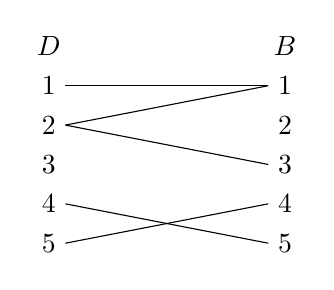
\begin{tikzpicture}
		%Nodes
		\node (Left_Over) 	at (0,0.5) 		{$D$};
		\node (Left_1) 		at (0,0) 		{$1$};
		\node (Left_2) 		at (0,-0.5) 	{$2$};
		\node (Left_3) 		at (0,-1) 		{$3$};
		\node (Left_4) 		at (0,-1.5) 	{$4$};
		\node (Left_5) 		at (0,-2) 		{$5$};
		\node (Right_Over) 	at (3,0.5) 		{$B$};
		\node (Right_1) 		at (3,0) 		{$1$};
		\node (Right_2) 		at (3,-0.5) 	{$2$};
		\node (Right_3) 		at (3,-1) 		{$3$};
		\node (Right_4) 		at (3,-1.5) 	{$4$};
		\node (Right_5) 		at (3,-2) 		{$5$};

		%Verkn�pfungen
		\draw (Left_1.east) -- (Right_1.west);
		\draw (Left_2.east) -- (Right_1.west);
		\draw (Left_2.east) -- (Right_3.west);
		\draw (Left_4.east) -- (Right_5.west);
		\draw (Left_5.east) -- (Right_4.west);
		\end{tikzpicture}
		\end{minipage}\\
		keine Abbildung
		\begin{itemize}
		\item da von $2$ zwei Pfeile weggehen ($> 1$)
		\item da von $3$ kein Pfeil weggeht
		\end{itemize}

\item Falls $D, B$ endliche Mengen gilt
		\[\betrag{f [D]} \leqq \betrag{D}\]
\renewcommand{\labelenumi}{\arabic{enumi}.}}

\subsection{Injektiv, Surjektiv, Bijektiv}
Eine Abbildung $\vert$ Funktion $f: D \rightarrow B, x \mapsto f(x)$ hei�t
\begin{enumerate}
\item injektiv, falls f�r alle $x,x' \in D$, $x \neq x'$ gilt $f(x) \neq f(x')$
\item surjektiv, falls es f�r jedes $y \in B$ ein $x \in D$ gibt mit $f(x) = y$, falls also $f [D] = B$
\item bijektiv, falls $f$ injektiv und surjektiv ist
\end{enumerate}

\textalignenum{Beispiel:}{}{
\begin{multicols}{2}
\renewcommand{\labelenumi}{\alph{enumi})}
\item $ $\newline %TODO -- Fix the top/bottom/middle problem
		%IMG-23.10.2008-mathe-3
		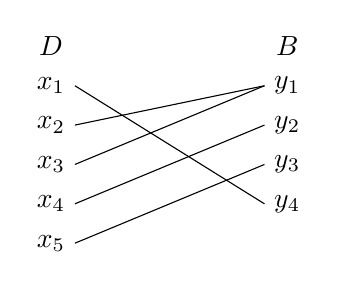
\begin{tikzpicture}
		%Nodes
		\node (Left_Over) 	at (0,0.5) 		{$D$};
		\node (Left_1) 		at (0,0) 		{$x_1$};
		\node (Left_2) 		at (0,-0.5) 	{$x_2$};
		\node (Left_3) 		at (0,-1) 		{$x_3$};
		\node (Left_4) 		at (0,-1.5) 	{$x_4$};
		\node (Left_5) 		at (0,-2) 		{$x_5$};
		\node (Right_Over) 	at (3,0.5) 		{$B$};
		\node (Right_1) 		at (3,0) 		{$y_1$};
		\node (Right_2) 		at (3,-0.5) 	{$y_2$};
		\node (Right_3) 		at (3,-1) 		{$y_3$};
		\node (Right_4) 		at (3,-1.5) 	{$y_4$};

		%Verkn�pfungen
		\draw (Left_1.east) -- (Right_4.west);
		\draw (Left_2.east) -- (Right_1.west);
		\draw (Left_3.east) -- (Right_1.west);
		\draw (Left_4.east) -- (Right_2.west);
		\draw (Left_5.east) -- (Right_3.west);
		\end{tikzpicture}
		\begin{itemize}
		\item nicht injektiv $(f(x_2) = f(x_3))$
		\item surjektiv
		\item nicht bijektiv
		\end{itemize}

\item $ $\newline %TODO -- Fix the top/bottom/middle problem
		%IMG-23.10.2008-mathe-4
		\begin{minipage}{50mm}
		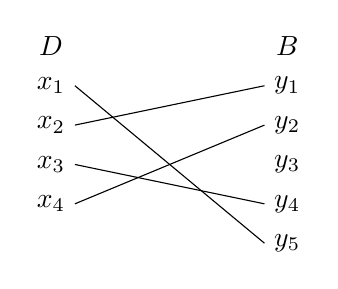
\begin{tikzpicture}
		%Nodes
		\node (Left_Over) 	at (0,0.5) 		{$D$};
		\node (Left_1) 		at (0,0) 		{$x_1$};
		\node (Left_2) 		at (0,-0.5) 	{$x_2$};
		\node (Left_3) 		at (0,-1) 		{$x_3$};
		\node (Left_4) 		at (0,-1.5) 	{$x_4$};
		\node (Right_Over) 	at (3,0.5) 		{$B$};
		\node (Right_1) 		at (3,0) 		{$y_1$};
		\node (Right_2) 		at (3,-0.5) 	{$y_2$};
		\node (Right_3) 		at (3,-1) 		{$y_3$};
		\node (Right_4) 		at (3,-1.5) 	{$y_4$};
		\node (Right_5) 		at (3,-2) 		{$y_5$};

		%Verkn�pfungen
		\draw (Left_1.east) -- (Right_5.west);
		\draw (Left_2.east) -- (Right_1.west);
		\draw (Left_3.east) -- (Right_4.west);
		\draw (Left_4.east) -- (Right_2.west);
		\end{tikzpicture}
		\end{minipage}
		\begin{itemize}
		\item injektiv
		\item nicht surjektiv $(y_3 \notin f [D])$
		\item nicht bijektiv
		\end{itemize}

\item $ $\newline %TODO -- Fix the top/bottom/middle problem
		%IMG-23.10.2008-mathe-5
		\begin{minipage}{50mm}
		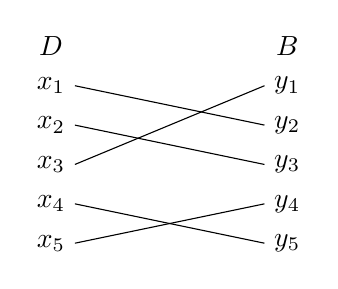
\begin{tikzpicture}
		%Nodes
		\node (Left_Over) 	at (0,0.5) 		{$D$};
		\node (Left_1) 		at (0,0) 		{$x_1$};
		\node (Left_2) 		at (0,-0.5) 	{$x_2$};
		\node (Left_3) 		at (0,-1) 		{$x_3$};
		\node (Left_4) 		at (0,-1.5) 	{$x_4$};
		\node (Left_5) 		at (0,-2) 		{$x_5$};
		\node (Right_Over) 	at (3,0.5) 		{$B$};
		\node (Right_1) 		at (3,0) 		{$y_1$};
		\node (Right_2) 		at (3,-0.5) 	{$y_2$};
		\node (Right_3) 		at (3,-1) 		{$y_3$};
		\node (Right_4) 		at (3,-1.5) 	{$y_4$};
		\node (Right_5) 		at (3,-2) 		{$y_5$};

		%Verkn�pfungen
		\draw (Left_1.east) -- (Right_2.west);
		\draw (Left_2.east) -- (Right_3.west);
		\draw (Left_3.east) -- (Right_1.west);
		\draw (Left_4.east) -- (Right_5.west);
		\draw (Left_5.east) -- (Right_4.west);
		\end{tikzpicture}
		\end{minipage}
		\begin{itemize}
		\item injektiv
		\item surjektiv
		\item bijektiv
		\end{itemize}

\item $ $\newline %TODO -- Fix the top/bottom/middle problem
		%IMG-23.10.2008-mathe-6
		\begin{minipage}{50mm}
		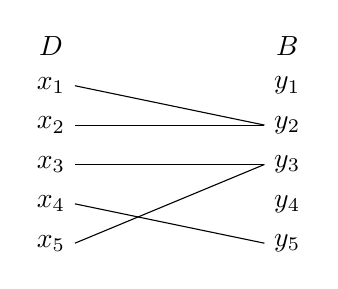
\begin{tikzpicture}
		%Nodes
		\node (Left_Over) 	at (0,0.5) 		{$D$};
		\node (Left_1) 		at (0,0) 		{$x_1$};
		\node (Left_2) 		at (0,-0.5) 	{$x_2$};
		\node (Left_3) 		at (0,-1) 		{$x_3$};
		\node (Left_4) 		at (0,-1.5) 	{$x_4$};
		\node (Left_5) 		at (0,-2) 		{$x_5$};
		\node (Right_Over) 	at (3,0.5) 		{$B$};
		\node (Right_1) 		at (3,0) 		{$y_1$};
		\node (Right_2) 		at (3,-0.5) 	{$y_2$};
		\node (Right_3) 		at (3,-1) 		{$y_3$};
		\node (Right_4) 		at (3,-1.5) 	{$y_4$};
		\node (Right_5) 		at (3,-2) 		{$y_5$};

		%Verkn�pfungen
		\draw (Left_1.east) -- (Right_2.west);
		\draw (Left_2.east) -- (Right_2.west);
		\draw (Left_3.east) -- (Right_3.west);
		\draw (Left_4.east) -- (Right_5.west);
		\draw (Left_5.east) -- (Right_3.west);
		\end{tikzpicture}
		\end{minipage}
		\begin{itemize}
		\item $f_4$ ist nicht injektiv $(f(x_1) = f(x_2))$
		\item $f_4$ ist nicht surjektiv $y_1 \notin f [D]$
		\item $f_4$ ist nicht nicht bijektiv
		\end{itemize}
\renewcommand{\labelenumi}{\arabic{enumi}.}
\end{multicols}}

\subsection{Hintereinanderausf�hrung}
Seien $f: D \rightarrow B$ und $g: B \rightarrow W$ zwei Funktionen/Abbildungen. Dann ist die Hintereinanderausf�hrung $g \circ f: D \rightarrow W$ (''$g$ verkn�pft mit $f$'', ''$g$ nach $f$'') der Abbildungen $f$ und $g$ definiert durch
\[x \mapsto (g \circ f) (x) := g (f(x))\]
\textalign{Beispiel:}{Gegeben Funktionen $f, g$ gesucht $g \circ f$
\[f \overbrace{\gklamm{1, 2, 3, 4, 5}}^{D :=} \rightarrow \overbrace{\gklamm{1, 2, 3, 4}}^{B :=}\]
\[f(1) = f(2) := 2, f(3) := 3, f(4) = f(5) := 4\]
\\
\[g \overbrace{\gklamm{1, 2, 3, 4}}^{B :=} \rightarrow \overbrace{\gklamm{1, 2, 3, 4, 5, 6}}^{W :=}\]
\[g(1) := 1, g(2) = g(3) := 2, g(4) := 6\]
%IMG-23.10.2008-mathe-7
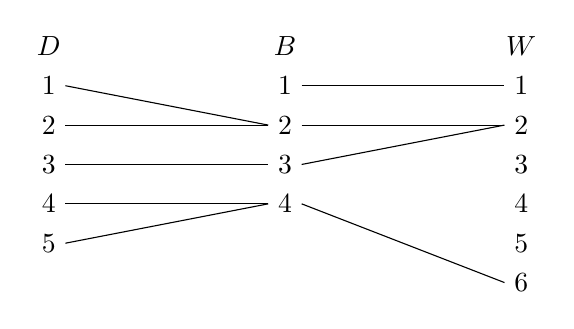
\begin{tikzpicture}
%Nodes
\node (Left_Over) 	at (0,0.5) 		{$D$};
\node (Left_1) 		at (0,0) 		{$1$};
\node (Left_2) 		at (0,-0.5) 	{$2$};
\node (Left_3) 		at (0,-1) 		{$3$};
\node (Left_4) 		at (0,-1.5) 	{$4$};
\node (Left_5) 		at (0,-2) 		{$5$};

\node (Center_Over) 	at (3,0.5) 		{$B$};
\node (Center_1) 		at (3,0) 		{$1$};
\node (Center_2) 		at (3,-0.5) 	{$2$};
\node (Center_3) 		at (3,-1) 		{$3$};
\node (Center_4) 		at (3,-1.5) 	{$4$};

\node (Right_Over) 	at (6,0.5) 		{$W$};
\node (Right_1) 		at (6,0) 		{$1$};
\node (Right_2) 		at (6,-0.5) 	{$2$};
\node (Right_3) 		at (6,-1) 		{$3$};
\node (Right_4) 		at (6,-1.5) 	{$4$};
\node (Right_5) 		at (6,-2) 		{$5$};
\node (Right_6) 		at (6,-2.5) 	{$6$};

%Verkn�pfungen
\draw (Left_1.east) -- (Center_2.west);
\draw (Left_2.east) -- (Center_2.west);
\draw (Left_3.east) -- (Center_3.west);
\draw (Left_4.east) -- (Center_4.west);
\draw (Left_5.east) -- (Center_4.west);

\draw (Center_1.east) -- (Right_1.west);
\draw (Center_2.east) -- (Right_2.west);
\draw (Center_3.east) -- (Right_2.west);
\draw (Center_4.east) -- (Right_6.west);
\end{tikzpicture}\\
%IMG-23.10.2008-mathe-8
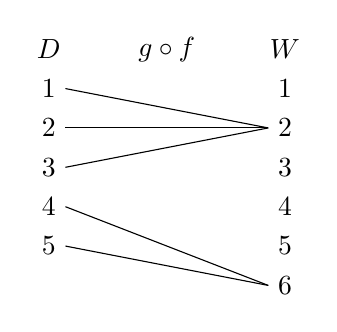
\begin{tikzpicture}
%Nodes
\node (Left_Over) 	at (0,0.5) 		{$D$};
\node (Left_1) 		at (0,0) 		{$1$};
\node (Left_2) 		at (0,-0.5) 	{$2$};
\node (Left_3) 		at (0,-1) 		{$3$};
\node (Left_4) 		at (0,-1.5) 	{$4$};
\node (Left_5) 		at (0,-2) 		{$5$};

\node (Right_Over) 	at (3,0.5) 		{$W$};
\node (Right_1) 		at (3,0) 		{$1$};
\node (Right_2) 		at (3,-0.5) 	{$2$};
\node (Right_3) 		at (3,-1) 		{$3$};
\node (Right_4) 		at (3,-1.5) 	{$4$};
\node (Right_5) 		at (3,-2) 		{$5$};
\node (Right_6) 		at (3,-2.5) 	{$6$};

%Beschriftungen
\node (Besch_1) at (1.5,0.5) {$g \circ f$};

%Verkn�pfungen
\draw (Left_1.east) -- (Right_2.west);
\draw (Left_2.east) -- (Right_2.west);
\draw (Left_3.east) -- (Right_2.west);
\draw (Left_4.east) -- (Right_6.west);
\draw (Left_5.east) -- (Right_6.west);
\end{tikzpicture}\\

$f: D \rightarrow B, g: B \rightarrow W$\\
$g \circ f: D \rightarrow W$\\
\textalign{Bemerkung:}{
Auch wenn $D = B = W$ gilt allgemein: $g \circ f \neq f \circ $g}}

\textalign{Beispiel:}{$D =B = W = \relmeng$
\begin{alignat*}{2}
	\func{f}&\relmeng \ra \relmeng~~\func{g}&&\relmeng \ra \relmeng\\
	&x \mapsto x^2 &&x \mapsto x - 1
\end{alignat*}
\begin{itemize}
\item $(f \circ g) (x) = f(g(x)) = f(x-1) =(x-1)^2$\\
		ab. z.B $(f \circ g) (2) = (2-1)^2 = 1$
\item $(g \circ f)(x) = g (f(x)) = g (x^2) = x^2 -1$\\
		$(g \circ f)(2) = 2^2 - 1 = 3$\\
		$\Ra (f \circ g) (2) \neq (g \circ f) (2)$\\
		$\Ra f \circ g \neq g \circ f$
\end{itemize}}
\subsection{Umkehrabbildungen}
\label{Def-Umkehrabbildungen}
Sind $D$ und $B$ nichtleere Mengen und $\func{f} D \ra B, x \mapsto f(x)$ eine bijektive Funktion/Abbildung, so gibt es zu jedem $y \in B$ genau ein $x \in D$ mit $x = f(x)$. Man kann daher die folgende Abbildung definieren.
\begin{align*}
	\func{f^{-1}}~&B \ra D\\
	&y \mapsto f^{-1} (y) = x
\end{align*}
Diese Abbildung hei�t Umkehrfunktion von $f$.

\section{S�tze}
Sei $A$ eine nichtleere Menge und $R$ eine �quivalenzrelation auf $A$. Dann gilt f�r beliebige $a, b \in A$
\begin{enumerate}
\item die beiden �quivalenzklassen $[a]$ und $[b]$ sind gleich $([a] = [b])$ oder disjunkt $([a] \cap [b] = \emptyset)$\\
		zu zeigen falls $[a] \cap [b] \neq \emptyset \Ra [a] = [b]$\\
		wir zeigen zun�chst $[a] \subseteq [b]$\\
		$[a] \cap [b] \neq \emptyset \Ra \exists r \in ([a] \cap [b])$
		$x \in [a]$ beliebig
		\[x \thicksim a \und a \thicksim r \underbrace{\Ra}_{\mbox{transitiv}} x \thicksim r\]
		\[x \thicksim r \und r \thicksim b \underbrace{\Ra}_{\mbox{transitiv}} x \thicksim b\]
		\[\Ra x \in [b]\]
		\[\Ra [a] \subseteq [b]\]
		analog zeigt man $[b] \subseteq [a]$\\
		\demonstrand{$\Ra [a] = [b]$}
\item $\bigcup_{a \in A} \{a\} = A$\\
		Beweis: wegen der Reflexivit�t von $R$ gilt f�r jedes $a \in A~~a \in [a]$ und damit
		\[\left.\begin{array}{l}
		\bigcup_{a \in A} [a] \supseteq \bigcup_{a \in A} {a} = A\\
		\mbox{aber}\\
		\bigcup_{a \in A} [a] \subseteq \bigcup_{a \in A} A = A
		\end{array}\right\} \Ra \bigcup_{a \in A} [a] = A\]
\end{enumerate}
\textalignenum{Beispiel:}{}{
\item Auf der Menge $A = \relmeng$ beziehungsweise $\mathbb{Z, Q, R}$ ist durch die nat�rliche Ordnung $a \subseteq b$, $a,b \in A$ eine Totalordnung definiert.
\item Auf der Menge $A = \relmeng$ ist durch $n \vert m$ (''$n$ teilt $m$'', ''$n$ ist Teiler von'', $n \vert m$ hei�t $\exists k \in \relmeng$, so dass $m = n k)$ eine Ordnungsrelation definiert.
		\begin{itemize}
		\item reflexiv $\checkmark$
		\item antisymmetrisch
				\begin{align*}
				&n \vert m \und m \vert n\\
				&m = n \mal k_1 n = m \mal k_2\\
				&m = (m \mal k_2) k_1\\
				\Leftrightarrow ~&k_1 \mal k_2 = 1\\
				\Rightarrow ~&m = n
				\end{align*}
		\item transitiv $\checkmark$
		\end{itemize}
		vollst�ndig $\Leftrightarrow (m, n) \in R$ oder $(n, m) \in R$\\
		die Ordnung $R$ ist nicht vollst�ndig,\\
		da z.B. $(5,6) \notin R$ und $(6,5) \notin R$
		also $\begin{array}{l} 5 \mbox{ ist kein Teiler von } 6 \mbox{ und}\\6 \mbox{ ist kein Teiler von } 5\end{array}$\\
		daher $5$ und $6$ sind nicht vergleichbar bez�glich der Teilbarkeit}

\textalign{Verwendung:}{Immer wenn Listen sortiert werden sollten, muss f�r die Inhalte der Liste eine Totalordnung gegeben sein.}

\subsection{Klasseneinteilung einer Menge}
Sei $A$ eine nichtleere Menge und $\RM{1}$ eine nichtleere Indexmenge. Weiter gelte:
\begin{itemize}
\item $\forall i \in \RM{1}~~K_i \neq \emptyset, K_i \subseteq A$
\item $\forall i,j \in \RM{1}$ mit $i \neq j$: $K_i \cap K_j = \emptyset$
\item $A = \bigcup_{i \in \RM{1}} K_i$
\end{itemize}
Eine derartige Darstellung von $A$ als Vereinigung von nichtleeren disjunkten Teilmengen $K_i \subseteq A$, $i \in \RM{1}$ nennt man Klasseneinteilung der Menge $A$.\\
F�r $a, b \in A$ gelte $a \thicksim b$ falls es ein $i \in \RM{1}$ gibt mit $a, b \in K_j$. Dann ist $\thicksim$ eine �quivalenzrelation auf der Menge $A$ mit �quivalenzklassen $K_i$, $i \in \RM{1}$.\\
Beweis: nachpr�fend Eigenschaften einer �quivalenzrelation\\
\textalignenum{Beispiel:}{}{
\item Klassifizierung der B�cher in der FH-Bibliothek\\
		Klassen:
		\begin{itemize}
		\item Matheb�cher 
		\item Informatikb�cher
		\item Elektrotechnikb�cher
		\end{itemize}
		\renewcommand{\labelitemi}{$\Rightarrow$}
		\begin{itemize}
		\item die Klassen sind disjunkt (jedes Buch kann nur an einer Stelle stehen)
		\item die Vereinigung aller Klassen entspricht dem gesamten Bestand der Bibliothek
		\end{itemize}
		\renewcommand{\labelitemi}{$\bullet$}
		Die �quivalenzrelation (also 2 B�cher derselben Klasse sind �quivalent) erlaubt es auch einem Laien die B�cher zu sortieren.

\item Restklassen\\
		Die Relation $R$ auf den ganzen Zahlen ist definiert durch
		\[R := \gklamm{(n, m) \in \ganzmeng \times \ganzmeng \vert n - m \mbox{ ist ein Vielfaches von} 7}\]
		dies ist eine �quivalenzrelation\\
		Klasseneinteilung
		\begin{alignat*}{2}
			&[0] &&= \gklamm{\dots, -14, -7, 0, 7, 14, 21, 28, \dots}\\
			&[1] &&= \gklamm{\dots, -13, -6, 1, 8, 15, 22, 29, \dots}\\
			&[2] &&= \gklamm{\dots, -12, -5, 2, 9, 16, 23, 30, \dots}\\
			&&\vdots\\
			&[6] &&= \gklamm{\dots, -15, -8, -1, 6, 13, 20, 27, \dots}
		\end{alignat*}}

\textalignenum{Anwendung:}{}{
\item Wochentage
		\begin{alignat*}{2}
			&[0] &&\equals \mbox{ Sonntage}\\
			&[1] &&\equals \mbox{ Montage}
		\end{alignat*}
		Heute ist der Mittwoch 22.10, welcher Wochentag ist in einem Monat also am 22.11\\
		\[ \left[ \underbrace{3}_{\mbox{heute Mittwoch}} + \underbrace{31}_{\mbox{Oktoberl�nge}} \right] = \lbrack 34 \rbrack = \lbrack 6 \rbrack \equals \mbox{ Samstag}\]
		\[\Ra \mbox{ am 22.11 ist also ein Samstag}\]

\item Pr�fziffern\\
		alte ISBN Zahlen $\underbrace{a_1, a_2, \dots, a_9}_{9 \mbox{ Ziffern}}, \underbrace{b}_{\mbox{Pr�fziffern}} = c$
		\begin{alignat*}{2}
			&b &&= \overbrace{\left[a_1 \mal 1 + a_2 \mal 2 + a_3 \mal 3 + \dots + a_9 \mal 9\right]_{11}}^{:= c}\\
			&b &&\equals \mbox{ Rest der Zahl $c$ bei der Division durch}
		\end{alignat*}
		\[\begin{array}{lcllcl}
		[0]  & = 		& \{0, 11, 22, 33, \dots\} 	& \Ra b 	& = 		& 0\\[0pt]
		     & \vdots 	& 										& 			& \vdots &	\\[0pt]
		[9]  & = 		& \{9, 20, \dots\} 				& 			& \vdots &	\\[0pt]
		[10] & = 		& \{10, 21, 32, 43, \dots\} 	& \Ra b 	& = 		& \RM{10}
		\end{array}\]
		die Pr�fziffer �ndert sich bei Vertauschung benachbarter Ziffern.}

\subsection{Satz zu Umkehrabbildungen}
\label{sec:Grundlagen-1-24}
Sind $D$ und $B$ nichtleere Mengen und $\func{f} D \ra B, x \mapsto f(x)$ eine bijektive Funktion, sowie $f^{-1}$ die Umkehrfunktion von $f$, so gilt:
\begin{enumerate}
\item $\forall x \in D\!\!:\; \left(f^{-1} \circ f\right) (x) = x$
\item $\forall y \in B\!\!:\; \left(f \circ f^{-1}\right) (y) = y$
\end{enumerate}
Folgt aus \vref{Def-Umkehrabbildungen}\\
\textalign{Bemerkung:}{
Statt $\forall x \in D\!\!:\; \left(f^{-1} \circ f\right) (x) = x$ schreibt man auch $f^{-1} \circ f = id_D$\\
$id_D$ hei�t die Identit�t auf der Menge $D$.}

\textalignmize{Anwendungen:}{}{
\item Speichern ($f$) einer Textdatei als Folge von Nullen und Einsen, Laden der entsprechenden Daten ($f^{-1}$).
\item Umwandlung von Sprache in �bertragbare elektromagnetische Wellen im Telefon (und den entsprechenden reversiblen Vorgang).}

\section{Aufgaben}
\subsection{Aufgabe 1.4}
\label{sec:Aufgabe-RelationenUndAbbildungen-EinsPunktVier}
Es sei $R$ die Relation auf $A := $\gklamm{1, 2, 3, 4}, die dadurch definiert ist, dass $xRy$ genau dann gilt, wenn $x + 2y$ ungerade ist. Stellen sie $R$ auf jede der folgenden Arten dar:
\renewcommand{\labelenumi}{\alph{enumi})}
\begin{enumerate}
\item als Menge geordneter Paare
\item als gerichteten Graphen
\item als Matrix
\end{enumerate}
\renewcommand{\labelenumi}{\arabic{enumi}.}

L�sung siehe \vref{sec:Loesung-RelationenUndAbbildungen-EinsPunktVier}.

\subsection{Aufgabe 1.5}
\label{sec:Aufgabe-RelationenUndAbbildungen-EinsPunktFuenf}
Entscheiden sie, welche der folgenden Relationen auf der Menge der Menschen reflexiv, symmetrisch oder transitiv ist:
\renewcommand{\labelenumi}{\alph{enumi})}
\begin{enumerate}
\item \quotate{hat die selben Eltern wie}
\item \quotate{ist Bruder von}
\item \quotate{ist �lter als}
\end{enumerate}
\renewcommand{\labelenumi}{\arabic{enumi}.}

L�sung siehe \vref{sec:Loesung-RelationenUndAbbildungen-EinsPunktFuenf}.

\chapter{Vollst�ndige Induktion}
Die Vollst�ndige Induktion ist ein Beweisprinzip, mit dem man Aussagen der Form $A(n)$ mit $n \in \natmeng$ beweisen kann.\\
Eine Anwendung ist der Nachweis der Korrektheit eines Algorithmuses.
\section{S�tze}
Sei $A(n)$ eine Aussage, die von $n \in \natmeng$ abh�ngt. Weiter seien ($IA$) und ($IS$) erf�llt, wobei Induktionsanfang ($IA$) : $A(1)$ ist richtig\\
Induktionsschluss $(IS) : \forall n \in \natmeng : A(n) \Ra A(n+1)$\\
Dann gilt die Aussage $A(n)$ f�r alle $n \in \natmeng$

\textalign{Beweis:}{
\[\underbrace{A(1)}_{\equals (IA)} \overbrace{\Ra}^{\equals (IS) \mbox{ f�r } n = 1} A(2) \underbrace{\Ra}_{\equals (IS) \mbox{ f�r } n = 2} A(3)\overbrace{\Ra}^{\equals (IS) \mbox{ f�r } n = 3} A(4) \Ra \dots\]}

\textalignmize{Bemerkungen:}{}{
\item $(IA)$ bezeichnet man auch als Verankerung
\item Da man im Induktionsschluss verwenden muss, dass $A(n)$ gilt, bezeichnet man die Aussage, dass $A(n)$ gilt auch als Induktionsvoraussetzung ($IV$)
\item Das Prinzip der vollst�ndigen Induktion kann man auch auf Aussagen $A(k)$ mit\\
		$k \in \gklamm{k_0, k_0 + d, k_0 + 2d, k_0 + 3d, \dots}$ mit $d \in \relmeng$\\
		($IA$) $A(k_0)$ ist richtig \dots\\
		\dots ($IS$) f�r alle $n \in \natmeng$ gilt $\underbrace{A(k_0 + nd)}_{=: \widetilde{A} (n)} \Ra \underbrace{A(k_0 + (n+1)d)}_{=: \widetilde{A} (n + 1)}$}

\textalignenum{Beispiel:}{}{
\item Behauptung: $\forall b \in \natmeng$: $1 + 2 + 3 + 4 \dots + (n -1) + n = \frac{n (n+1)}{2}$\\
\begin{align*}
		(IA) &n = 1 ~~ LS = 1, RS = \frac{1 (1 + 1)}{2} = 1 \checkmark\\
		(IS) &z.z \forall n \in \natmeng: \overbrace{1 + 2 + \dots + (n - 1) + n = \frac{n \mal (1+n)}{2}}^{(IV)}\\
		&\Ra 1 + 2 + 3 + \dots + (n -1) + n + (n+1) = \frac{(n+2) (n+1)}{2}\\
		(IV) &\frac{n \mal (n +1)}{2} + (n + 1)\\
		&= (n+1) \left( \frac{n}{2} + 1 \right) = (n + 1) \frac{n+2}{2} = \frac{(n+1) (n+2)}{2}\\
\end{align*}
\item Beweis von Satz \vref{sec:VerallgemeinerteRegelnvondeMorgan} Verallgemeinerte Morgan Regeln\\
		Behauptung: Seien $A_1, A_2, A_3, \dots \subseteq M$, so gilt:\\
		$\forall n \in \natmeng \overline{\bigcup_{k = 1}^{n} A_k} = \bigcap_{k = 1}^{n} \overline{A_k}$\\
		Beweis:\\
		$(IA) n = 1~~LS = \overline{\bigcup_{k=1}^1 A_k} = \overline{A_1}, RS= \bigcap_{k=1}^1 \overline{A_k} = \overline{A_1} \checkmark$
		$n = 2~~ \left.\begin{array}{l}LS = \overline{\bigcup_{k=1}^2 A_k} = \overline{A_1 \cup A_2} = \overline{A_1} \cap \overline{A_2}\\RS = \bigcap_{k=1}^2 \overline{A_k} = \overline{A_1} \cap \overline{A_2}\end{array}\right\}\checkmark$
		$(IS)$}

\textalign{Behauptung:}{$1^3 + 2^3 + 3^3 + \dots + (n-1)^3 + n^3 = \left( \frac{n (n + 1)}{2} \right)^2$\\
$(IA) n = 1 LS = 1^3 = 1$\\
$RS = \left( \frac{1 ( 1+ 1)}{2} \right)^2 = 1^2 = 1 \checkmark$\\
$(IS) z.z. (\mbox{zu zeigen}) \forall n \in \natmeng: \overbrace{1^3 +2^3 + 3^3 + \dots n^3 = \left( \frac{n (n+1)}{2} \right)^2}^{(IV)}$\\
$\Ra 1^3 + 2^3 + 3^3 \dots + n^3 + (n + 1)^3 = \left( \frac{(n+1)(n+2)}{2} \right)^2$\\
$\left( 1^3 + 2^3 +3^3 + \dots + n^3 + (n + 1)^3 \right)$\\
$(IV) \left( \frac{n ( n + 1)}{2} \right)^2 + (n + 1)^3$\\
$= (n + 1)^3 \left(\frac{n^2 + (n+1)^2}{2^2} \right)$\\
$= (n + 1)^2 \frac{n^2 + 4n + 4}{4} = \frac{(n+2)^2 (n+1)^2}{2^2}$\\
\demonstrand{$= \left(\frac{(n+1)(n+2)}{2} \right)^2$}}

\section{Definitionen}
\subsection{Rekursive Definition}
\textalign{Bemerkung:}{Rekursive Definitionen folgen dem gleichen Prinzip wie die vollst�ndige Induktion.}

\textalign{Beispiel:}{F�r jedes $n \in \natmeng_0$ ist $n!$ die Fakult�t von $n$ definiert durch:
\begin{alignat*}{2}
	&n! := 1 &&\mbox{f�r } n = 0\\
	&n! := (n-1)! \mal n &&\mbox{f�r } n \in \natmeng\\
\end{alignat*}}

\textalign{Anwendung:}{Z�hlen von Anzahlen bei Permutation}

\textalign{Beispiel:}{wie viele Anordnungen der Ziffern $1, 2, 3$ gibt es?
\[\begin{array}{l}
123\\
132\\
213\\
231\\
312\\
321
\end{array}\]
\begin{itemize}
\item F�r die erste Stelle gibt es 3 M�glichkeiten
\item Dann bleiben an der zweiten Stelle noch 2 M�glichkeiten �brig
\item Dann bleibt f�r die letzte Stelle nur noch 1 M�glichkeit �brig
\end{itemize}
$3 \mal 2 \mal 1 = 6$}

\section{Aufgaben}
\subsection{A16}
\label{sec:Aufgabe-VollstaendigeInduktion-A16}
TODO: Nachtragen der Aufgabenstellung

L�sung siehe \vref{sec:Loesung-VollstaendigeInduktion-A16}.

\chapter{\texorpdfstring{$\sum$-Notation und $\prod$-Notation}{Summen-Notation und Produkt-Notation}}
\section{\texorpdfstring{Definition $\sum$-Notation}{Definition Summen-Notation}}
\label{sec:DefinitionSummenNotation}
\[\sum_{k = 1}^1 a_k := a_1\]
\[\sum_{k = 1}^{n + 1} a_k := \left(\sum_{k = 1}^n a_k\right) + a_{n+1} \mbox{ f�r } n \in \natmeng\]
wobei man $k$ als Laufindex/Summationsindex bezeichnet.
\subsection{\texorpdfstring{Definition $\prod$-Notation}{Definition Produkt-Notation}}
\label{sec:DefinitionProduktNotation}
\[\prod_{k = 1}^1 a_k := a_1\]
\[\prod_{k = 1}^{n + 1} a_k := \left(\prod_{k = 1}^n a_k\right) \mal a_{n+1} \mbox{ f�r } n \in \natmeng\]
Bemerkung:
\begin{enumerate}
\item Salopp geschrieben\\
		$\sum_{k=1}^n a_k = a_1 + a_2 + a_3 + \dots + a_{n-1} + a_n$ \\
		$\prod_{k=1}^n a_k = a_1 \mal a_2 \mal a_3 \mal \dots \mal a_{n-1} \mal a_n$
\item Der Name des Laufindex ist unwichtig\\
		$\sum_{k=1}^n a_k = \sum_{l=1}^n a_l$ \\
		$\prod_{k=1}^n a_k = \prod_{l=1}^n a_l$
\item Im Fall $m>n$ vereinbart man\\
		$\sum_{k=m}^n a_k := 0$ leere Summe\\
		$\prod_{k=m}^n a_k := 1$ leeres Produkt
\item $\sum_{k=1}^n a_k = \sum_{1 \leqq k \leqq n} a_k$\\
		$\prod_{l=1}^n a_l = \prod_{1 \leqq l \leqq n} a_l$
\end{enumerate}
\renewcommand{\labelenumi}{Bsp. \arabic{enumi}.}
\begin{enumerate}
\item Summe aller Quadrate von ungeraden nat�rlichen Zahlen kleiner als $100$
		\[\sum_{1 \leqq k \leqq 99} k^2 = \sum_{l = 0}^{49} (2l + 1)^2\]
\item Die Fakult�t kann man damit folgenderma�en schreiben
		\[n! := 1 \mbox{ f�r } n = 0\]
		\[n! := \prod_{k = 1}^n k \mbox{ f�r } n \in \natmeng\]
\end{enumerate}
\renewcommand{\labelenumi}{\arabic{enumi}.}

\section{\texorpdfstring{Rechenregeln f�r $\sum, \prod$}{Rechenregeln f�r Summen und Produktnotationen}}
\begin{enumerate}
\item $\sum_{k = 1}^n a_k + \sum_{k = n+1}^m a_k = \sum_{k = 1}^m a_k$\\
		$(\prod_{k = 1}^n a_k) (\prod_{k = n+1}^m a_k) = \prod_{k = 1}^m a_k$
\item $\sum_{k=1}^n (a_k + b_k) = \left( \sum_{k = 1}^n a_k \right) + \left( \sum_{k = 1}^n b_k \right)$ \\
		$\prod_{k=1}^n (a_k \mal b_k) = \left( \prod_{k = 1}^n a_k \right) \mal \left( \prod_{k = 1}^n b_k \right)$
\item $\sum_{k=1}^n t \mal a_k = t \mal \left( \sum_{k=1}^n a_k \right)$
\item Indexverschiebung\\
		$\underbrace{\sum_{k=1}^n a_k}_{a_1 + a_2 + \dots + a_n} = \underbrace{\sum_{l=0}^{n - 1}}_{a_1 + a_2 + \dots + a_n} = \sumx{l = m + 1}{n + m}{a_{l-m}}$\\
		$\prodx{k = 1}{n}{a_k} = \prodx{l=0}{n-1}{a_{l+1}} = \prodx{l = m+1}{n+m}{a_{l -m}}$
\item Inversion der Reihenfolge\\
		$\sumx{k=1}{n}{a_k} = \sumx{k=1}{n}{a_{n+1-k}}$\\
		$\prodx{k=1}{n}{a_k} = \prodx{k=1}{n}{a_{n+1 - k}}$\\
		Beweis: Folgt aus \vref{sec:DefinitionSummenNotation} und \ref{sec:DefinitionProduktNotation}\\
		Bemerkung: Alternative Schreibweise f�r Indexverschiebung\\
		\[\sumx{k=1}{n}{a_k} = \sumx{1 \leqq k \leqq n}{}{a_k} = \sumx{1 \leqq l+1 \leqq n}{}{a_{l+1}} = \sumx{0 \leqq l \leqq n-1}{}{a_{l+1}} = \sumx{l=0}{n-1}{a_{l+1}}\]
\end{enumerate}

\chapter{K�rper}
Ein K�rper ist eine algebraische Struktur, in der zwei Verkn�pfungen ''$+$'' und ''$\mal$'' definiert sind.\\
In $\mathbb{Q}$ und in $\relmeng$ stimmen die Rechenregeln mit den bekannten �berein.
\section{Definitionen}
\subsection{K�rper}
Ein K�rper $K$ ist eine nichtleere Menge zusammen mit zwei inneren Verkn�pfungen
\begin{alignat*}{2}
	''+'': &K \times K \ra K ~~~''\mal'': &&K \times K \ra K\\
	&(x, y) \mapsto x + y &&(x,y) \mapsto x \mal y
\end{alignat*}
die folgenden Gesetze (K�rperaxiome) erf�llen
\subsubsection{Addition}
\begin{itemize}
\item Assoziativgesetz
		\[\forall x,y,z \in K: (x +y) + z = x+(y+z)\]
\item Kommutativgesetz
		\[\forall x,y \in K: x + y = y +x\]
\item Neutrales Element\\
		es gibt genau ein Nullelement $0 \in K$
		\[\forall x \in K: 0 + x = x\]
\item Inverses Element\\
		F�r jedes $x \in K \exists! (-x) \in K$ so dass $x+(-x)=0$
\end{itemize}
\subsection{Multiplikation}
\begin{itemize}
\item Assoziativgesetz
		\[\forall x, y, z \in K: (x \mal y) \mal z = x \mal (y \mal z)\]
\item Kommutativgesetz
		\[\forall x, y \in K: x \mal y = y \mal x\]
\item Neutrales Element\\
		es existiert ein neutrales Element (Einselement) $1 \in K \backslash \gklamm{0}$, so dass f�r alle $x \in K \backslash \gklamm{0}$: x \mal 1 = x
\item Inverses Element\\
		zu jedem $x \in K \backslash \gklamm{0} \exists! x^{-1} \in K: x \mal x^{-1} = 1$
\end{itemize}
\subsection{Distributivgesetz}
\[\forall x, y \in K: x \mal (y + z) = (x \mal y) + (x \mal z)\]
Bemerkung:
\begin{enumerate}
\item Schreibweise:
		\[a \mal b = ab\]
		\[(a \mal b) + (c \mal d) = ab + cd \mbox{ (''Punkt vor Strich'')}\]
\item In jedem K�rper gelten die bekannten Rechenregeln
		\begin{enumerate}
		\item $\forall x \in K: 0 \mal x = 0$
		\item $\forall x,y \in K \backslash \gklamm{0}: x \mal y \neq 0$
		\end{enumerate}
\end{enumerate}
Beispiel:
\begin{enumerate}
\item $\mathbb{Q}$, kleinster K�rper, der alle nat�rlichen Zahlen enth�lt
\item $\mathbb{R}$, gr��ter K�rper auf dem man eine Totalordnung definieren kann
\item $\mathbb{Q} (\sqrt{2}) := \gklamm{a + b \sqrt{2} \vert a, b \in \mathbb{Q}}$\\
		\begin{itemize}
		\item Abgeschlossenheit bez�glich Addition\\
		\[a_1 + b_1 \sqrt{2} \in \mathbb{Q} (\sqrt{2})\]
		\[a_2 + b_2 \sqrt{2} \in \mathbb{Q} (\sqrt{2})\]
		\[\left(a_1 + b_2 \sqrt{2}\right) + \left(a_2 + b_2 \sqrt{2}\right) = \underbrace{\left(a_1 + a_2\right) + \left(b_1 + b_2\right) \sqrt{2}}_{\in \mathbb{Q}(\sqrt{2})}\]
		Assoziativgesetz der Addition $\checkmark$\\
		Kommutativgesetz der Addition $\checkmark$\\
		Nullelement: $0 + 0 \sqrt{2}$\\
		Inverses Element der Addition: Inverses von $a + b \sqrt{2}$ ist $-a -b \sqrt{2}$
		\item Abgeschlossenheit bez�glich Multiplikation
		\begin{alignat*}{2}
			a_1 + b_1\sqrt{2} \in \mathbb{Q}(\sqrt{2})\\
			a_2 + b_2\sqrt{2} \in \mathbb{Q}(\sqrt{2})
		\end{alignat*}
		$(a_1 + b_1 \sqrt{2}) \mal (a_2 + b_2 \sqrt{2})$\\
		$a_1 a_2 + a_1 b_2 \sqrt{2} + a_2 b_1 \sqrt{2} + b_1 b_2 \underbrace{\sqrt{2} \sqrt{2}}_{=2}$\\
		$(a_1 \mal a_2 + b_1 \mal b_2) + (a_1 b_2 + a_2 b_1)\sqrt{2}$\\
		Assoziativgesetz der Multiplikation $\checkmark$\\
		Kommutativgesetz der Multiplikation $\checkmark$\\
		Nullelement: $1 + 0 \sqrt{2}$\\
		Inverses Element der Multiplikation: Inverses von $(a + b \sqrt{2}) \mal (a + b \sqrt{2})^{-1} = 1$\\
		$(a + b \mal \sqrt{2})^{-1} = \frac{1}{a + b \sqrt{2}} = \frac{a - b \sqrt{2}}{(a + b \sqrt{2})(a - b \sqrt{2})}$\\
		$\frac{a - b \sqrt{2}}{a^2 - b^2 2} = \frac{a}{a^2 - 2b^2} + \frac{-b}{a^2 - 2b^2} \sqrt{2} \in \mathbb{Q} (\sqrt{2})$\\
		Distributivgesetz $\checkmark$
\end{itemize}
\item $\mathbb{C} = \gklamm{a + b i \vert a, b \in \mathbb{R}, i^2 = -1}$\\
		K�rper der komplexen Zahlen
\item $F_2 := \gklamm{0, 1}$\\
		Ein K�rper muss zumindest das Nullelement und das Einselement enthalten\\
		\begin{tabular}{c||c|c}
		$+$ & $0$ & $1$\\
		\hline \hline
		$0$ & $0$ & $1$\\
		\hline
		$1$ & $1$ & $0$\\
		\hline
		\end{tabular}
		\begin{tabular}{c||c|c}
		$\mal$ & $0$ & $1$\\
		\hline \hline
		$0$ & $0$ & $0$\\
		\hline
		$1$ & $0$ & $1$\\
		\hline
		\end{tabular}
\item $F_3 = \gklamm{0, 1, 2}$\\
		\begin{minipage}{10cm}
		\begin{tabular}{c||c|c|c}
		$+$ & $0$ & $1$ & $2$\\
		\hline \hline
		$0$ & $0$ & $1$ & $2$\\
		\hline
		$1$ & $1$ & $2$ & $0$\\
		\hline
		$2$ & $2$ & $0$ & $1$\\
		\hline
		\end{tabular}
		An $(-1) = 1 (-2) =2$\\
		$1 + 2 = 1$\\
		$(-1) + 1 + 2 = (-1) + 1$\\
		$2 = 0$
		\end{minipage}
		\begin{minipage}{10cm}
		\begin{tabular}{c||c|c|c}
		$\mal$ & $0$ & $1$ & $2$\\
		\hline \hline
		$0$ & $0$ & $0$ & $0$\\
		\hline
		$1$ & $0$ & $1$ & $2$\\
		\hline
		$2$ & $0$ & $2$ & $1$\\
		\hline
		\end{tabular}
		$x \in \gklamm{0, 1, 2}$\\
		$x \neq 0$ da $\underbrace{2}_{\neq 0} \mal \underbrace{2}_{\neq 0} \neq 0$\\
		da $2 \mal 2^{-1} = 1$\\
		$\Ra 2^{-1} = 2$
		\end{minipage}
\item $F_p$ Restklassenk�rper bez�glich der Primzahl $p$.\\
		Anwendung: F�r gro�e $p$ Verwendung in der Codierung
\end{enumerate}


\part{Lineare Gleichungssysteme}
\chapter{Motivation, �quivalenzumformung}
\renewcommand{\labelenumi}{Bsp \arabic{enumi}.}
\begin{enumerate}
\item Eine Gruppe von Leuten bestellt im Caf� f�r jeden ein Getr�nk
		\begin{description}
		\item[Kaffee] kostet 2,50 \EUR
		\item[Tee] kostet 2,00 \EUR
		\end{description}
		Es trinken doppelt so viele Leute Kaffee wie Tee. Die Rechnung betr�gt 14,00 \EUR. Wie viele Personen sind in der Gruppe?
		\begin{align*}
		\mbox{L�sung: } &\mbox{Anzahl Teetrinker } t\\
							 &\mbox{Anzahl Kaffeetrinker } k
		\end{align*}
		\begin{align}
		2,5k + 2t &= 14 (\RM{1})\\
				 2t &= k (\RM{2})
		\end{align}
		\begin{alignat*}{2}
		\mbox{($\RM{2}$) in ($\RM{1}$) } &2,5k + k &&= 14\\
		&\Leftrightarrow 3,5k &&= 14\\
		&\Leftrightarrow k &&= \frac{14}{7} \mal 2\\
		&\mbox{in ($\RM{2}$)} 2t &&= 4\\
		&\Leftrightarrow t &&= 2
		\end{alignat*}
		$\Ra$ es sind 6 Leute in der Gruppe
\item 8 Personen sitzen im Caf� und jeder trinkt ein Getr�nk\\
		\begin{description}
		\item[Tee] kostet 2,00 \EUR
		\item[Schokolade] kostet 3,00 \EUR
		\item[Kaffee] kostet 2,50 \EUR
		\end{description}
		Rechnung betr�gt 19,00 \EUR\\
		Wie viele Personen trinken was?
		\begin{align*}
		\mbox{L�sung: } &\mbox{Anzahl Teetrinker } t\\
							 &\mbox{Anzahl Kaffeetrinker } k\\
							 &\mbox{Anzahl Schokoladentrinker } s
		\end{align*}
		\begin{align}
		2t + 3s + 2,5k &= 19\\
				 t + s + k &= 8
		\end{align}
		$(s, t, k \in \mathbb{N}_0)$\\
		$(\RM{1}) k = 8 - s - t$\\
		$(\RM{2}) in (\RM{1}) 2t + 3s + \frac{5}{2} (8 - s - t) = 19$\\
		$\Leftrightarrow t-s=2$\\
		\begin{tabular}{|c|c|c}
		$s$ & $t$ & $k$\\
		\hline
		$0$ & $2$ & $6$\\
		$1$ & $3$ & $4$\\
		$2$ & $4$ & $2$\\
		$3$ & $5$ & $0$\\
		\end{tabular}\\
		d.h. es gibt keine eindeutige L�sung
\end{enumerate}
\renewcommand{\labelenumi}{\arabic{enumi}.}
Ziel:
\begin{itemize}
\item Erkenntnisse �ber L�sbarkeit (plus gegebenenfalls Anzahl der L�sungen) eines linearen Gleichungssystems.
\item Im Falle der L�sbarkeit ein einfaches (programmierbares) Verfahren
\end{itemize}
\section{Definitionen}
\subsection{Lineares Gleichungssystem}
\begin{itemize}
\item Eine lineare Gleichung in den Variablen $x_1, x_2, \dots, x_n$ ist eine Gleichung der Form
		\[a_1 \mal x_1 + a_2 \mal x_2 + a_3 \mal x_3 + \dots + a_{n-1} x_{n-1} + a_n \mal x_n = b\]
		dabei sind $b$ und die Koeffizienten $a_1, a_2, \dots, a_n$ aus einem K�rper $K$ (meistens $K = \mathbb{R}$).
\item Ein lineares Gleichungssystem besteht aus $m$ linearen Gleichungen in den Variablen $x_1, x_2, \dots, x_n$:
		\begin{alignat*}{2}
			&a_{11} \mal x_1 + a_{12} \mal x_2 + a_{13} \mal x_3 + \dots + a_{1 n-1} \mal x_{n-1} + a_{1n} \mal x_n &&= b_1\\
			&a_{21} \mal x_1 + a_{22} \mal x_2 + a_{23} \mal x_3 + \dots + a_{2 n-1} \mal x_{n-1} + a_{2n} \mal x_n &&= b_2\\
			&\vdots &\vdots\\
			&a_{m1} \mal x_1 + a_{m2} \mal x_2 + a_{m3} \mal x_3 + \dots + a_{m n-1} \mal x_{n-1} + a_{mn} \mal x_n &&= b_m
		\end{alignat*}
\item Eine L�sung des Gleichungssystems ist ein $n$-Tupel von Zahlen aus $K$ ($s_1, s_2, s_3, \dots, s_n$) mit der Eigenschaft, dass alle $m$ Gleichungen des Systems wahre Aussagen werden, wenn man statt $x_j \mal s_j$ ($1 \leq j \leq n$) einsetzt.
\item Die Menge aller L�sungen eines linearen Gleichungssystems hei�t L�sungsmenge.
\item Zwei lineare Gleichungssysteme hei�en �quivalent, wenn sie dieselbe L�sungsmenge haben.
\end{itemize}
\begin{description}
\item[Bemerkung:] Eine lineare Gleichung in 2 Variablen $a_1 x + a_2 y = b$ beschreibt eine Gerade, d.h. L�sungen dieser Gleichung sind alle Punkte ($s_1, s_2$) die auf dieser Geraden liegen.\\
						Wenn wir zwei Gleichungen $a_{11} x + a_{12} y = b_1$ und $a_{21} x + a_{22} y = b_2$ in zwei Variablen haben, entspricht die L�sungsmenge der Menge aller Punkte, die auf beiden Geraden liegen $(a_1, a_2, a_{11}, a_{12}, a_{21}, a_{22}, b, b_1, b_2 \in \mathbb{R})$
						damit ergibt sich
						\begin{enumerate}
						\item 0 L�sungen falls die beiden Geraden parallel sind
						\item 1 L�sung wenn sich die Geraden schneiden (allgemeiner Fall)
						\item unendlich viele L�sungen, falls die beiden Gleichungen dieselbe Gerade beschreiben
						\end{enumerate}
						Diese F�lle sind auch f�r lineare Gleichungssysteme mit $m$ Gleichungen in $n$ Variablen mit Koeffizienten in $\mathbb{R}$ die einzig m�glichen.
\end{description}
\subsection{Konsistent, Inkonsistent}
Ein Gleichungssystem hei�t konsistent, wenn es L�sungen hat und inkonsistent wenn es keine L�sungen hat.

\subsection{(Erweiterte) Koeffizientenmatrix}
Die Daten eines linearen Gleichungssystems mit $m$ Gleichungen in $n$ Variablen
\begin{alignat*}{2}
	&a_{11} \mal x_1 + a_{12} \mal x_2 + \dots + a_{1 n-1} \mal x_{n-1} + a_{1n} \mal x_{n} &&= b_1\\
	&a_{21} \mal x_1 + a_{22} \mal x_2 + \dots + a_{2 n-1} \mal x_{n-1} + a_{2n} \mal x_{n} &&= b_2\\
	&\vdots &&\vdots\\
	&a_{m1} \mal x_1 + a_{m2} \mal x_2 + \dots + a_{m n-1} \mal x_{n-1} + a_{mn} \mal x_{n} &&= b_m
\end{alignat*}
Kann man in der Koeffizientenmatrix
\[\left(\begin{array}{cccccc}
a_{11} & a_{12} & a_{13} & \dots & a_{1 n-1} & a_{1n}\\
a_{21} & a_{22} & a_{23} & \dots & a_{2 n-1} & a_{2n}\\
\vdots & \vdots & \vdots & \vdots& \vdots    & \vdots\\
a_{m1} & a_{m2} & a_{m3} & \dots & a_{m n-1} & a_{mn}
\end{array}\right)\]
darstellen beziehungsweise in der erweiterten Koeffizientenmatrix
\[\left(\begin{array}{cccccc|c}
a_{11} & a_{12} & a_{13} & \dots & a_{1 n-1} & a_{1n} & b_1\\
a_{21} & a_{22} & a_{23} & \dots & a_{2 n-1} & a_{2n} & b_2\\
\vdots & \vdots & \vdots & \vdots& \vdots    & \vdots\\
a_{m1} & a_{m2} & a_{m3} & \dots & a_{m n-1} & a_{mn} & b_m
\end{array}\right)\]
\subsection{Elementare Zeilenumformungen}
Die folgenden Operationen hei�en elementare Zeilenumformungen einer Matrix.\\
\begin{description}
\item[Ersetzen] Addition des $\lambda$-fachen ($\lambda \in K$) der Zeile $j$ zur Zeile $i$ ($i \neq j$)
		\begin{alignat*}{2}
			i = 1 ~~(\RM{1}) \longrightarrow (\RM{1}) + \lambda(\RM{2})\\
			i = 2 ~~(\RM{2}) \longrightarrow (\RM{2})
		\end{alignat*}
		Beispiel:
		$\begin{array}{cc|c}
		2 & 4 & 1\\
		0 & -2 & 2\\
		\end{array}\underrightarrow{\RM{1} = \RM{1} + 2 \RM{2}}
		\begin{array}{cc|c}
		2 & 0 & 5\\
		0 & -2 & 2
		\end{array}$
\item[Vertauschen] Vertauschen der Zeilen $i$ und $j$
		\begin{align*}
			i = 1 ~~(\RM{1}) \longrightarrow (\RM{2})\\
			j = 2 ~~(\RM{2}) \longrightarrow (\RM{1})
		\end{align*}
		Beispiel:
		$\begin{array}{cc|c}
		0 & -7 & 2\\
		3 & 1 & 1\\
		\end{array}\underrightarrow{\RM{1} <-> \RM{2}}
		\begin{array}{cc|c}
		3 & 1 & 1\\
		0 & -7 & 2
		\end{array}$
\item[Skalieren] Multiplikation der $i$-ten Zeile mit einem Faktor $\lambda \in K$ ($\lambda \neq 0$)
		\begin{align*}
			i = 1 ~~&(\RM{1}) \longrightarrow (\RM{1} \mal \lambda)\\
			&(\RM{2}) \longrightarrow (\RM{2})
		\end{align*}
		Beispiel:
		$\begin{array}{cc|c}
		2 & 0 & 5\\
		0 & -2 & 2\\
		\end{array}\underrightarrow{\RM{2} = \RM{2} \mal \left(\frac{1}{2}\right)}
		\begin{array}{cc|c}
		2 & 0 & 5\\
		0 & 1 & -1
		\end{array}$\\
		Zwei Matrizen, die durch eine Reihe von elementaren Zeilenoperationen ineinander �berf�hrt werden k�nnen, hei�en zeilen�quivalent.
\end{description}
\section{S�tze}
Sind die erweiterten Koeffizientenmatritzen zweier linearer Gleichungssysteme zeilen�quivalent, so stimmen die L�sungsmengen der Gleichungssysteme �berein.

\chapter{Gausssches Eliminationsverfahren}
\section{(Reduzierte) Zeilenstufenform}
\begin{enumerate}
\item Eine Matrix ist in Zeilenstufenform, wenn gilt:
		\renewcommand{\labelenumii}{\roman{enumii})}
		\begin{enumerate}
		\item Alle Nullzeilen (daher Zeilen, die nur aus Nullen bestehen) stehen am Ende der Matrix
		\item Der erste Eintrag (Koeffizient) ungleich 0 in jeder Zeile steht rechts vom ersten Eintrag ungleich 0 der dar�ber liegenden Zeile
		\end{enumerate}
		\renewcommand{\labelenumii}{\alph{enumii}.}
		Der erste Eintrag ungleich 0 einer Zeile nennt man Pivot-Element. Die Spalten, die ein Pivot-Element enthalten nennt man Pivot-Spalten.\\
		\textalign{Beispiel:}{$ $\newline %TODO -- Fix the top/bottom/middle problem
		\renewcommand{\labelenumii}{\arabic{enumii})}
		\begin{enumerate}
		\item $\gauss{ccc}{
				\textcolor{blue}{1} & 2 & 0\\
				0 & \textcolor{blue}{1} & 1\\
				\textcolor{red}{\uparrow} & \textcolor{red}{\uparrow} &}$

		\item $\gauss{ccccc}{
				\textcolor{blue}{2} & 3 & 1 & 7 & 1\\
				0 & \textcolor{blue}{1} & 2 & 8 & 3\\
				0 & 0 & \textcolor{blue}{3} & 6 & 2\\
				0 & 0 & 0 & 0 & \textcolor{blue}{1}\\
				\textcolor{red}{\uparrow} & \textcolor{red}{\uparrow} & \textcolor{red}{\uparrow} & & \textcolor{red}{\uparrow}}$

		\item $\gauss{cccc}{
				0 & \textcolor{blue}{1} & 2 & 9\\
				0 & 0 & 0 & \textcolor{blue}{3}\\
				0 & 0 & 0 & 0\\
				0 & 0 & 0 & 0\\
				&\textcolor{red}{\uparrow} & & \textcolor{red}{\uparrow}}$\\\\
				\textcolor{blue}{0 Pivot Element}\\
				\textcolor{red}{1 Pivot-Spalten}%TODO: linien die die nuller abgrenzen in den arrays
		\end{enumerate}
		\renewcommand{\labelenumii}{\alph{enumii}.}}

\item Eine Matrix ist in reduzierter Zeilenstufenform, wenn sie in Zeilenstufenform ist und zudem gilt:
		\renewcommand{\labelenumii}{\roman{enumii})}
		\begin{enumerate}
		\item Alle Pivot-Elemente sind gleich $1$
		\item Alle Eintr�ge �ber Pivot-Elementen sind gleich $0$
		\end{enumerate}
		\renewcommand{\labelenumii}{\alph{enumii}.}
\end{enumerate}
\textalign{Beispiel:}{$ $\newline %TODO -- Fix the top/bottom/middle problem
\begin{enumerate}
\item $\gauss{cc}{
		1 & 0\\
		0 & 1\\
		\uparrow & \uparrow
		}$

\item $\gauss{ccccc}{
		0 & 1 & 2 & 0 & 3\\
		0 & 0 & 0 & 1 & 4\\
		&\uparrow && \uparrow&
		}$

\item $\gauss{cccc}{
		1 & 5 & 0 & 3\\
		0 & 0 & 1 & 8\\
		0 & 0 & 0 & 0\\
		0 & 0 & 0 & 0\\
		\uparrow && \uparrow&
		}$
\end{enumerate}}
\section{Gaussverfahren}
\begin{enumerate}
\item Starte mit der Spalte am weitesten links, die nicht nur $0^{\mbox{en}}$ enth�lt. Dies ist die aktuelle Pivot-Spalte
\item W�hle ein von $0$ verschiedenes Element der aktuellen Pivot-Spalte als Pivot-Element aus. Vertausche die Zeilen so, dass das gew�nschte Pivot-Element in die erste Zeile zu stehen kommt.
\item Erzeuge mit Hilfe elementarer Zeilenumformungen ''Ersetzen'' Nullen unter dem Pivot-Element
\item Decke die Zeile mit dem Pivot-Element und alle dar�ber liegenden Zeilen zu.\\
		F�hre Schritt 1-3 mit der �brig gebliebenen Teilmatrix durch.\\
		Wiederhole den Prozess bis keine von $0$ verschiedenen Zeilen �brig bleiben.
\item Beginne bei dem am weitesten rechts stehenden Pivot-Element und fahre dann nach links fort.\\
		Ist ein Pivot-Element von $1$ verschieden, bringe es durch Skalierung auf $1$.\\
		Erzeuge durch ''Ersetzen'' lauter Nullen �ber dem Pivot-Element.\\
\end{enumerate}
\textalign{Bemerkung:}{Die Schritte 1-4 erzeugen die Zeilenstufenform und werden Vorw�rtsphase/-prozess\index{Vorw�rtsphase}\index{Vorw�rtsprozess} des Gaussverfahrens genannt.\\
	Der Schritt 5 erzeugt die reduzierte Zeilenstufenform und wird R�ckw�rtphase\index{R�ckw�rtphase} des Gaussverfahrens genannt.}
\textalign{Bemerkung:}{Wenn man das Gauss-Verfahren auf die erwartete Koeffizientenmatrix eines linearen Gleichungssystems anwendet, kann man dessen L�sungsmenge an der reduzierten Zeilenstufenform ablesen.}

\section{Definitionen}
\subsection{Basis Variable, freie Variable}
\label{sec:BasisVariable_freieVariable}
Sei $A$ eine erweiterte Koeffizientenmatrix eines linearen Gleichungssystems und $U$ die zu $A$ geh�rende reduzierte Zeilenstufenform, dann nennt man die zu Pivot-Spalten geh�renden Variablen Basis-Variablen\index{Basis-Variablen} und die anderen Variablen hei�en freie Variablen\index{Freie-Variablen}.

\section{S�tze}
\subsection{Eindeutigkeit der reduzierten Zeilenstufenform}
Jede Matrix ist zeilen�quivalent zu genau einer Matrix in reduzierter Zeilenstufenform
\subsubsection{Bezeichnung}
Wenn die Matrix $A$ zeilen�quivalent zur Matrix $U$ ist und $U$ sich in (reduzierter) Zeilenstufenform befindet, nennt man $U$ die (reduzierte) Zeilenstufenform von $A$.\\
\textalign{Beispiel:}{$ $\newline %TODO -- Fix the top/bottom/middle problem
$A =
\gauss{cccc}{
1 & 1 & 1 & 8\\
1 & -1 & -1 & 0\\
5 & 4 & 6 & 38}$

soll in reduzierte Zeilenstufenform gebracht werden.\bigskip

\onehalfspacing$\gauss{cccc}{
1 & 1 & 1 & 8\\
1 & -1 & -1 & 0\\
5 & 4 & 6 & 38}$
$\underrightarrow{\RM{1} \leftrightarrow \RM{2}}
\gauss{cccc}{
5 & 4 & 6 & 38\\
1 & -1 & -1 & 0\\
1 & 1 & 1 & 8}$
$\underrightarrow{\RM{1} = \RM{1} - 5 \RM{3}}
\gauss{cccc}{
0 & -1 & 1 & -2\\
1 & -1 & -1 & 0\\
1 & 1 & 1 & 8}$
$\underrightarrow{\RM{2} = \RM{2} + \RM{3}}
\gauss{cccc}{
0 & -1 & 1 & -2\\
2 & 0 & 0 & 8\\
1 & 1 & 1 & 8}$
$\underrightarrow{\RM{2} = \RM{2} \frac{1}{2}}
\gauss{cccc}{
0 & -1 & 1 & -2\\
1 & 0 & 0 & 4\\
1 & 0 & 2 & 6}$
$\underrightarrow{\RM{1} \leftrightarrow \RM{2}}
\gauss{cccc}{
1 & 0 & 0 & 4\\
0 & -1 & 1 & -2\\
1 & 0 & 2 & 6}$
$\underrightarrow{\RM{3} = \RM{3} - \RM{1}}
\gauss{cccc}{
1 & 0 & 0 & 4\\
0 & -1 & 1 & -2\\
0 & 0 & 2 & 2}$
$\underrightarrow{\RM{2} = \RM{2} \mal  (-1)}
\gauss{cccc}{
1 & 0 & 0 & 4\\
0 & 1 & -1 & 2\\
0 & 0 & 2 & 2}$
$\underrightarrow{\RM{3} = \RM{3} \mal \frac{1}{2}}
\gauss{cccc}{
1 & 0 & 0 & 4\\
0 & 1 & -1 & -2\\
1 & 0 & 1 & 1}$
$\underrightarrow{\RM{2} = \RM{2} + \RM{3}}
\gauss{cccc}{
1 & 0 & 0 & 4\\
0 & 1 & 0 & 3\\
0 & 0 & 1 & 1}$
$\Leftrightarrow
\begin{array}{ccc}
x_1 = 4\\
x_2 = 3\\
x_3 = 1
\end{array}$\singlespacing}
\subsection{Existenz und Eindeutigkeit der L�sung}
\label{sec:ExistenzundEindeutigkeitderLoesung}
$A, U$ wie in \vref{sec:BasisVariable_freieVariable}, dann gilt:
\begin{enumerate}
\item Das lineare Gleichungssystem ist genau dann konsistent, wenn die letzte Spalte von $U$ keine Pivot-Spalte ist.
\item Wenn das lineare Gleichungssystem konsistent ist, ist die L�sung genau dann eindeutig, wenn es keine freien Variablen gibt.
\end{enumerate}
\newcounter{beispielcounter}
\textalign{Beispiel:}{
\addtocounter{beispielcounter}{1}
\textalign{\arabic{beispielcounter}.}{
		\onehalfspacing$\begin{array}{rcrcr}
		2x & + & y & = & -1\\
		-x & + & 3y & = & 0\\
		2x & + & 8y & = & -2
		\end{array}$
		$\Leftrightarrow
		\gauss{cc|c}{
		2 & 1 & -1\\
		-1 & 3 & 0\\
		2 & 8 & -2
		}$
		$\underrightarrow{\RM{1} \leftrightarrow \RM{2}}
		\gauss{cc|c}{
		-1 & 3 & 0\\
		2 & 1 & -1\\
		2 & 8 & -2
		}$
		$\underrightarrow{\RM{2} = \RM{2} + 2 \RM{1}}
		\gauss{cc|c}{
		-1 & 3 & 0\\
		0 & 7 & -1\\
		2 & 8 & -2
		}$
		$\underrightarrow{\RM{3} = \RM{3} + 2 \RM{1}}
		\gauss{cc|c}{
		-1 & 3 & 0\\
		0 & 7 & -1\\
		0 & 14 & -2
		}$
		$\underrightarrow{\RM{2} = \RM{3} - 2 \RM{2}}
		\gauss{cc|c}{
		-1 & 3 & 0\\
		0 & 7 & -1\\
		0 & 0 & 0
		}$
		$\underrightarrow{\RM{2} = \RM{2} \mal \frac{1}{7}}
		\gauss{cc|c}{
		-1 & 3 & 0\\
		0 & 1 & - \frac{1}{7}\\
		0 & 0 & 0
		}$
		$\underrightarrow{\RM{1} = \RM{1} - 3 \RM{2}}
		\gauss{cc|c}{
		-1 & 0 & \frac{3}{7}\\
		0 & 1 & -\frac{1}{7}\\
		0 & 0 & 0
		}$
		$\underrightarrow{\RM{3} = \RM{3} + 2 \RM{1}}
		\gauss{cc|c}{
		1 & 0 & - \frac{3}{7}\\
		0 & 1 & -\frac{1}{7}\\
		0 & 0 & 0\\
		\uparrow & \uparrow &
		}$\\
		$x = - \frac{3}{7}, y = - \frac{1}{7} \Leftrightarrow L = \gklamm{\left(- \frac{3}{7}, -\frac{1}{7}\right)}$\singlespacing}}

\textfakealign{Beispiel:}{
\addtocounter{beispielcounter}{1}
\textalign{\arabic{beispielcounter}.}{
		\onehalfspacing$\begin{array}{rcrcr}
		2x & + & y & = & -1\\
		-x & + & 3y & = & 0\\
		2x & + & 8y & = & -1
		\end{array} \Leftrightarrow
		\gauss{cc|c}{
		2 & 1 & -1\\
		-1 & 3 & 0\\
		2 & 8 & -1
		}$\\
		$\underrightarrow{\RM{1} \leftrightarrow \RM{2}}
		\gauss{cc|c}{
		-1 & 3 & 0\\
		2 & 1 & -1\\
		2 & 8 & -1
		}$
		$\underrightarrow{\RM{2} = \RM{2} - 2 \RM{1}}
		\gauss{cc|c}{
		-1 & 3 & 0\\
		0 & 7 & -1\\
		2 & 8 & -1
		}$\\
		$\underrightarrow{\RM{3} = \RM{3} - 2 \RM{1}}
		\gauss{cc|c}{
		-1 & 3 & 0\\
		0 & 7 & -1\\
		0 & 14 & -1
		}\underrightarrow{\RM{3} = \RM{3} - 2 \RM{2}}
		\gauss{cc|c}{
		-1 & 3 & 0\\
		0 & 7 & -1\\
		0 & 0 & 1\\
		&&\uparrow
		}$\\
		$\Ra \begin{array}{rcrcrl}
		-x & + & 3y & = & 0 &\\
		0x & + & 7y & = & -1&\\
		0x & + & 0y & = & 1 &\Leftarrow \mbox{ Immer Falsch}
		\end{array}$\\
		$\Ra$ keine L�sung beziehungsweise $L = \emptyset$\singlespacing}}

\textfakealign{Beispiel:}{
\addtocounter{beispielcounter}{1}
\textalign{\arabic{beispielcounter}.}{
		\onehalfspacing$\gauss{ccc|c}{
		2 & 1 & -1 & -1\\
		-1 & -1 & 3 & 0
		}\underrightarrow{\RM{1} \leftrightarrow \RM{2}}
		\gauss{ccc|c}{
		-1 & -1 & 3 & 0\\
		2 & 1 & -1 & -1
		}$\\
		$\underrightarrow{\RM{2} = \RM{2} + 2 \RM{1}}
		\gauss{ccc|c}{
		-1 & -1 & 3 & 0\\
		0 & -1 & 5 & -1
		}\underrightarrow{\RM{2} = \RM{2} \mal (-1)}
		\gauss{ccc|c}{
		-1 & -1 & 3 & 0\\
		0 & 1 & -5 & 1
		}$\\
		$\underrightarrow{\RM{1} = \RM{1} + \RM{2}}
		\gauss{ccc|c}{
		-1 & 0 & -2 & 1\\
		0 & 1 & -5 & 1
		}$
		$\underrightarrow{\RM{1} = \RM{1} \mal (-1)}
		\gauss{ccc|c}{
		1 & 0 & 2 & -1\\
		0 & 1 & -5 & 1\\
		\uparrow & \uparrow & &
		}$\\
		$\Ra x_1 x_2$ Basis Variable\\
		$\Ra x_3$ freie Variable\\
		$\Leftrightarrow \begin{array}{l}
		x_1 + 2 x_3 = -1\\
		x_2 - 5 x_3 = 1
		\end{array}$\\
		$L = \gklamm{\left(-1 - 2 \mal x_3, 1 + 5 x_3, x_3\right) \vert x_3 \in \mathbb{R}}$\\
		daher $x_1, x_2$ (Basis Variable) sind Funktionen der freien Variable $x_3$\singlespacing}}

\textalign{Beispiel:}{
\addtocounter{beispielcounter}{1}
\textalign{\arabic{beispielcounter}.}{
		\onehalfspacing$\gauss{cccc|c}{
		-1 & -2 & 1 & -1 & 2\\
		3 & 6 & -1 & 3 & 0
		}$
		$\underrightarrow{\RM{2} = \RM{2} + 2 \RM{1}}
		\gauss{cccc|c}{
		-1 & -2 & 1 & -1 & 2\\
		0 & 0 & 2 & 0 & 6
		}$
		$\underrightarrow{\RM{2} = \RM{2} \left(\frac{1}{2}\right)}
		\gauss{cccc|c}{
		-1 & -2 & 1 & -1 & 2\\
		0 & 0 & 1 & 0 & 3
		}$
		$\underrightarrow{\RM{1} = \RM{1} - \RM{2}}
		\gauss{cccc|c}{
		-1 & -2 & 0 & -1 & -1\\
		0 & 0 & 1 & 0 & 3
		}$
		$\underrightarrow{\RM{1} = \RM{1} \mal (-1)}
		\gauss{cccc|c}{
		1 & 2 & 0 & 1 & 1\\
		0 & 0 & 1 & 0 & 3\\
		\textcolor{blue}{\uparrow} & \textcolor{blue}{\uparrow} & \textcolor{blue}{\uparrow} & \textcolor{blue}{\uparrow} &
		}$
		$\Leftrightarrow
		\begin{array}{l}
		x_1 + 2s + t = 1\\
		x_3 = 3
		\end{array}$\\
		Basis-Variable\\
		\textcolor{blue}{freie-Variable}\\
		$L = \gklamm{\left(1 - 2s - t, s, 3, t\right) \vert s, t \in \mathbb{R}}$\singlespacing}}
\section{Aufgaben}
\subsection{Aufgabe 2.1}
\subsubsection{Aufgabenstellung}
L�sen sie das folgende Gleichungssystem, indem sie die erweiterte Koeffizientenmatrix auf reduzierte Zeilenstufenform bringen.
\[\begin{array}{rrrrrrr}
2x & + & y & - & 3z & = & 0\\
6x & + & 3y & - & 8z & = & 0\\
2x & - & y & + & 5z & = & -4
\end{array}\]
\subsubsection{Aufgaben L�sung}
\[\gauss{ccc|c}{
2 & 1 & -3 & 0\\
6 & 3 & -8 & 0\\
2 & -1 & 5 & -4
}\underrightarrow{\RM{2} = \RM{2} - 3 \mal \RM{1}}
\gauss{ccc|c}{
2 & 1 & -3 & 0\\
0 & 0 & 1 & 0\\
2 & -1 & 5 & -4
}\underrightarrow{\RM{3} \leftrightarrow \RM{2}}
\gauss{ccc|c}{
2 & 1 & -3 & 0\\
2 & -1 & 5 & -4\\
0 & 0 & 1 & 0
}\]\\
\[\underrightarrow{\RM{2} = \RM{2} - \RM{1}}
\gauss{ccc|c}{
2 & 1 & -3 & 0\\
0 & -2 & 8 & -4\\
0 & 0 & 1 & 0
}\Leftrightarrow
\begin{array}{rcrcrcr}
2x & + & 1y & + & -3z & = & 0\\
&&-2y & + & 8z & = & -4\\
&&&&1z & = & 0
\end{array}\Rightarrow\]\\
\[\begin{array}{rl}
& z = 0\\
-2y = -4 \Ra & y = 2\\
2x + 2 - 0 = 0 \Ra & x = -1
\end{array}\]
\subsection{Aufgabe 2.2}
\subsubsection{Aufgabenstellung}
Bestimmen Sie alle L�sungen von:
\renewcommand{\labelenumi}{\alph{enumi})}
\begin{enumerate}
\item $\begin{array}{rcrcrcr}
		2x & + & y & - & 2z & = & 10\\
		3x & + & 2y & + & 2z & = & 1\\
		5x & + & 4y & + & 3z & = & 4
		\end{array}$

\item $\begin{array}{rcrcr}
		x & + & 2y & = & 4\\
		-2x & - & 3y & = & -6\\
		2x & + & y & = & 1
		\end{array}$

\item $\begin{array}{rcrcrcrcr}
		x_1 	& - & 2x_2 & + & 2x_3 	& - & x_4 	& = & 8\\
		3x_1 	& - & 7x_2 & + & x_4 	&				& = & 0
		\end{array}$
\end{enumerate}
\renewcommand{\labelenumi}{\arabic{enumi}.}

\subsubsection{Aufgaben L�sung}
\renewcommand{\labelenumi}{zu \alph{enumi})}
\begin{enumerate}
\item \onehalfspacing$\gauss{ccc|c}{
		2 & 1 & -2 & 10\\
		3 & 2 & 2 & 1\\
		5 & 4 & 3 & 4
		}$
		$\underrightarrow{\RM{2} = \RM{2} - \frac{3}{2} \RM{1}}
		\gauss{ccc|c}{
		2 & 1 & -2 & 10\\
		0 & \frac{1}{2} & 5 & -14\\
		5 & 4 & 3 & 4
		}$
		$\underrightarrow{\RM{3} = \RM{3} - \frac{5}{2} \RM{1}}
		\gauss{ccc|c}{
		2 & 1 & -2 & 10\\
		0 & \frac{1}{2} & 5 & -14\\
		0 & \frac{3}{2} & 8 & -21
		}$\\
		$\underrightarrow{\RM{3} = \RM{3} - 3 \RM{2}}
		\gauss{ccc|c}{
		2 & 1 & -2 & 10\\
		0 & \frac{1}{2} & 5 & -14\\
		0 & 0 & -7 & 21
		}$
		$\underrightarrow{\RM{3} = \RM{3} \frac{1}{7}}
		\gauss{ccc|c}{
		2 & 1 & -2 & 10\\
		0 & \frac{1}{2} & 5 & -14\\
		0 & 0 & 1 & -3
		}$
		$\underrightarrow{\RM{2} = \RM{2} - 5 \RM{3}}
		\gauss{ccc|c}{
		2 & 1 & -2 & 10\\
		0 & \frac{1}{2} & 0 & 1\\
		0 & 0 & 1 & -3
		}$\\
		$\underrightarrow{\RM{1} = \RM{1} + 2 \RM{2}}
		\gauss{ccc|c}{
		2 & 1 & 0 & 4\\
		0 & \frac{1}{2} & 0 & 1\\
		0 & 0 & 1 & -3
		}$
		$\underrightarrow{\RM{2} = \RM{2} \mal 2}
		\gauss{ccc|c}{
		2 & 1 & 0 & 4\\
		0 & 1 & 0 & 2\\
		0 & 0 & 1 & -3
		}$
		$\underrightarrow{\RM{1} = \RM{1} - \RM{2}}
		\gauss{ccc|c}{
		2 & 0 & 0 & 2\\
		0 & 1 & 0 & 2\\
		0 & 0 & 1 & -3
		}$\\
		$\underrightarrow{\RM{1} = \RM{1} \mal \frac{1}{2}}
		\gauss{ccc|c}{
		1 & 0 & 0 & 1\\
		0 & 1 & 0 & 2\\
		0 & 0 & 1 & -3
		}$
		$L \gklamm{(1, 2, -3)}$\singlespacing

\item $\gauss{cc|c}{
		1 & 2 & 4\\
		-2 & -3 & -6\\
		2 & 1 & 1}$
		$\underrightarrow{\RM{2} = \RM{2} + 2 \RM{1}}
		\gauss{cc|c}{
		1 & 2 & 4\\
		0 & 1 & 2\\
		2 & 1 & 1
		}$
		$\underrightarrow{\RM{3} = \RM{3} - 2 \RM{1}}
		\gauss{cc|c}{
		1 & 2 & 4\\
		0 & 1 & 2\\
		0 & -3 & -7}$
		$\underrightarrow{\RM{3} = \RM{3} + 3 \RM{2}}
		\gauss{ccc|c}{
		1 & 2 & 4\\
		0 & 1 & 2\\
		0 & 0 & -1\\
		&&\uparrow
		}$
		\[\Ra L = \emptyset\]

\item $\gauss{cccc|c}{
		1 & -3 & 2 & -1 & 8\\
		3 & -7 & & 1 & 0}$
		$\underrightarrow{\RM{2} = \RM{2} - 3 \RM{1}}
		\gauss{cccc|c}{
		1 & -3 & 2 & -1 & 8\\
		0 & 2 & -6 & 4 & -24
		}$
		$\underrightarrow{\RM{2} = \RM{2} \mal \frac{1}{2}}
		\gauss{cccc|c}{
		1 & -3 & 2 & -1 & 8\\
		0 & 1 & -3 & 2 & -12}$\\
		$\underrightarrow{\RM{1} = \RM{1} + 3 \RM{2}}
		\gauss{cccc|c}{
		1 & 0 & -7 & 5 & -28\\
		0 & 1 & -3 & 2 & -12\\
		\begin{sideways}BV\end{sideways} & \begin{sideways}BV\end{sideways} & \begin{sideways}fV\end{sideways} & \begin{sideways}fV\end{sideways}
		}$\\
		$L = \gklamm{\left(-28 + 7s -5t, -12 + 3s - 2t, s, t\right) \vert s, t \in \mathbb{R}}$
\end{enumerate}
\renewcommand{\labelenumi}{\arabic{enumi}.}

\subsection{Aufgabe 2.3}
\subsubsection{Aufgabenstellung}
In der Praxis treten oft sehr gro�e Gleichungssysteme auf. Dabei k�nnen Rundungsfehler starke Auswirkungen auf die L�sung der GLeichungen haben. Dies soll hier an einem einfachen Beispiel untersucht werden.
\renewcommand{\labelenumi}{\alph{enumi})}
\begin{enumerate}
\item 
\end{enumerate}
\renewcommand{\labelenumi}{\arabic{enumi}.}

\subsubsection{Aufgaben L�sung}
\renewcommand{\labelenumi}{\alph{enumi})}
\begin{enumerate}
\item 
\end{enumerate}
\renewcommand{\labelenumi}{\arabic{enumi}.}



\part{\texorpdfstring{Der Vektorraum, $\mathbb{R}^n$}{Der Vektorraum, R hoch n}}
\chapter{\texorpdfstring{Vektoren im $\mathbb{R}^n$}{Vektoren in R hoch n}}
Man interpretiert ein Element
\[\vec{x} = (x_1, x_2, x_3, \dots, x_n)^T = \vektor{x_1}{x_2}{x_3} \mbox{ mit } x \in \mathbb{R} \mbox{ f�r } 1 \leq i \leq n\]
\[\mbox{wobei hier } ()^T \mbox{ transponiert bedeutet}\]
des $\mathbb{R}^n$ als Vektor\index{Vektor} der vom Punkt $(0, 0, \dots, 0)^T$ (Koordinatenursprung$\vert$Nullpunkt) zum Punkt $(x_1, x_2, \dots, x_n)^T$ zeigt. Man nennt $\vec{x}$ auch Ortsvektor\index{Ortsvektor} des Punktes $(x_1, \dots, x_n)^T$.\\
$x_i$ nennt man $i$-te Koordinate\index{Koordinate} beziehungsweise $i$-te Komponente\index{Komponente} des Vektors/Punktes $\vec{x}$.\\
Man kann Vektoren auch parallel verschieben. Ist $(y_1, y_2, y_3, \dots y_n)^T \in \mathbb{R}^n$, so zeigt $\vec{x}$ vom Punkt $(y_1, y_2, \dots, y_n)^T$ zum Punkt $(y_1 + x_1, y_2 + x_2, \dots, y_n + y_n)^T$\\
%13.10.2008-IMG-mathe-1
\begin{tikzpicture}
%Koordinaten Achsen
\coordinate [label=left:{$2$}] (yend) at (0,3.5);
\coordinate [label=below:{$1$}] (xend) at (7,0);
\draw [->] (0,-0.25) -- (yend);
\draw [->] (-0.25,0) -- (xend);

\coordinate (ursprung) at (0,0);
\coordinate (ar1p1) at (1.5, 2.5);
\coordinate [label=right:{$\left(y_1 + x_1, y_2 + x_2\right)^T$}] (ar1p2) at (4.5,3.5);

\draw[->] (ursprung) -- (ar1p1);
\draw[->] (ar1p1) -- (ar1p2);
\node (bes11) at ($ (ursprung)!.5!(ar1p1) $) {};
\node (bes11t) at (1,3.5) {$\left(y_1, y_2\right)^T$};
\draw[->] (bes11t.south) -- (bes11.north);
\node [label=below:{$\vec{x}$}] (bes12) at ($ (ar1p1)!.5!(ar1p2) $) {};

\coordinate [label=right:{$\left(x_1, x_2\right)^T$}] (ar2p1) at (3,1);
\draw[->] (ursprung) -- (ar2p1);
\node [label=above:{$\vec{x}$}] (bes12) at ($ (ursprung)!.5!(ar2p1) $) {};

\node at (-1,1.75) {\huge{$\mathbb{R}^2$}};
\end{tikzpicture}\\
\textalign{Bemerkung:}{Man schreibt statt $\vec{x}$ auch $\underline{x}$, $\textbf{x}$}

\section{Definitionen}
\subsection{Vektoraddition und Multiplikation mit einem Skalar}
\label{sec:VektoradditionundMultiplikationmiteinemSkalar}
Seien $\vec{x} = (x_1, x_2, \dots, x_n)^T \in \mathbb{R}^n$ und $\vec{y} = (y_1, y_2, \dots, y_n)^T \in \mathbb{R}^n$ zwei Vektoren und $\lambda \in \mathbb{R}$ nennt man auch Skalar
\begin{enumerate}
\item $\vec{x} + \vec{y} = (x_1 + y_1, x_2 + y_2, \dots, x_n + y_n)^T = \vektor{x_1 + y_1}{x_2 + y_2}{x_n + y_n}$
\item $\lambda \mal \vec{x} = \lambda x_1, \lambda x_2, \lambda x_3, \dots, \lambda x_n)^T = \vektor{\lambda x_1}{\lambda x_2}{\lambda x_n}$
\item Nullvektor $\vec{0} = (0, 0, \dots, 0)^T$\\
		$-x = (-1) \mal \vec{x} = (-x_1, -x_2, -x_3, \dots, -x_n)^T = \vektor{-x_1}{-x_2}{-x_3}$\\
		es gilt $\vec{x} + \left(-\vec{x}\right) = (-x_1, -x_2, -x_3, \dots, -x_n) = \vektor{-x_1}{-x_2}{-x_3}$\\
		Man schreibt:
		\[\vec{y} - \vec{x} := \vec{y} + \left(-\vec{x}\right)\]
\end{enumerate}

\section {S�tze}
\subsection{\texorpdfstring{Algebraische Eigenschaften des $\mathbb{R}^n$}{Algebraische Eigenschaften des R hoch n}}
\label{sec:DerVektorraumRhochn-3-2}

$\vec{u}, \vec{v}, \vec{w} \in \mathbb{R}^n, \lambda, \mu \in \mathbb{R}$
\subsubsection{Vektor Addition}
\begin{enumerate}
\item Assoziativgesetz: $\left(\vec{u} + \vec{v}\right) + \vec{w} = \vec{u} + \left(\vec{v} + \vec{w}\right)$
\item Kommutativgesetz: $\vec{u} + \vec{v} = \vec{v} + \vec{u}$
\item Neutrales Element: $\vec{u} + \vec{0} = \vec{0} + \vec{u} = \vec{u}$
\item \textalign{Inverses Element:}{$\left(-\vec{u}\right) \mbox{ Inverses zu } \vec{u}$\\
		$\left(-\vec{u}\right) + \vec{u} = \vec{u} + \left(-\vec{u}\right) = \vec{0}$}
\end{enumerate}
\subsubsection{Vektor Multiplikation}
\begin{enumerate}
\item Assoziativgesetz: $(\lambda \mal \mu) \vec{u} = \lambda(\mu \mal \vec{u})$
\item (''Neutrales Element'') $1 \mal \vec{u} = \vec{u}$
\end{enumerate}
\subsubsection{Distributivgesetz}
\begin{enumerate}
\item $\lambda(\vec{u} + \vec{v}) = \lambda \mal \vec{u} + \lambda \vec{v}$
\item $(\lambda + \mu) \mal \vec{u} = \lambda \vec{u} + \mu \vec{u}$
\end{enumerate}
\textalign{Beweis:}{folgt aus Definition \vref{sec:VektoradditionundMultiplikationmiteinemSkalar} und den entsprechenden reellen Eigenschaften der Addition beziehungsweise Multiplikation.}

\input{kapitel/part_Vektorraum_R_hoch_n/kap_Lineare_Unabh�ngigkeit.tex}
\chapter{Lineare Abbildungen}
\section{Definitionen}
\subsection{Lineare Abbildung}
Seien $U \subseteq \mathbb{R}^n$ und $V \subseteq \mathbb{R}^m$ zwei Unterr�ume. Eine Abbildung $\func{f} U \ra V$ hei�t linear, falls sie f�r $\vec{x}, \vec{y} \in U, \lambda \in \mathbb{R}$ folgende Eigenschaften hat.
\begin{enumerate}
\item sie ist additiv\index{Additiv}, daher $f(\vec{x} + \vec{y}) = f(\vec{x}) + f(\vec{y})$
\item sie ist homogen\index{Homogen}, daher $f(\lambda \vec{x}) = \lambda \mal f(\vec{x})$
\end{enumerate}
\textalign{Bemerkung:}{
Aus 2. folgt$\underbrace{f (\vec{0}}_{\in \mathbb{R}^n)} = \underbrace{\vec{0}}_{\in \mathbb{R}^m}$\\
wobei $\vec{0}$ f�r ein Vektor $\in \mathbb{R}^n$ oder $\in \mathbb{R}^m$ steht.}

\subsection{Einheitsmatrix}
Sei $E_n$ eine $n \times n$-Matrix mit
\[E_n = \varvektor{cc}{1 & 0\\0 & 1}\]
$\left(E_n \mbox{ hat } 1^{\mbox{en}} \mbox{ auf der Diagonale, sonst nur }0^{\mbox{en}}\right)$\\
$E_n$ nennt man Einheitsmatrix\index{Einheitsmatrix}\\
Manchmal wird statt $E_n$ auch $I_n$ geschrieben

\subsection{Matrix-Vektor-Multiplikation}
\label{sec:MatrixVektorMultiplikation}
Sei $A = \varvektor{cccc}{a_{11} & a_{12} & \dots & a_{1n}\\a_{21} & a_{22} & \dots & a_{2n}\\\vdots & \vdots & \vdots & \vdots\\a_{31} & a_{32} & \dots & a_{3n}}$ eine $m \times n$ Matrix und\\
$\vec{v} = \vektor{v_1}{\vdots}{v_n} \in \mathbb{R}^n$, dann definiert man
\[A \mal \vec{v} = A\vec{v} = \varvektor{cccc}{a_{11} & a_{12} & \dots & a_{1n}\\a_{21} & a_{22} & \dots & a_{2n}\\\vdots & \vdots & \vdots & \vdots\\a_{31} & a_{32} & \dots & a_{3n}} \mal \vektor{v_1}{\vdots}{v_n} := \varvektor{c}{\sumx{j = 1}{n}{a_{1j} \mal v_j}\\\sumx{j = 1}{n}{a_{2j} \mal v_j}\\\vdots\\\sumx{j = 1}{n}{a_{mj} \mal v_j}} = \sumx{j = 1}{n}{\varvektor{c}{a_{1j} \mal v_j\\a_{2j} \mal v_j\\\vdots\\a_{mj} \mal v_j}}\]
\textalignenum{Beispiel:}{}{
\item $E_2 \varvektor{c}{2\\7} = \varvektor{cc}{1 & 0\\0 & 1} \mal \varvektor{c}{2\\7} = \varvektor{c}{1 \mal 2 + 0 \mal 7\\0 \mal 1 + 1 \mal 7} = \varvektor{c}{2\\7}$
\item $\varvektor{ccc}{1 & 2 & 3\\4 & 5 & 6} \mal \vektor{1}{0}{0} = \varvektor{c}{1 \mal 1 + 2 \mal 0 + 3 \mal 0\\4 \mal 1 + 5 \mal 0 + 6 \mal 0} = \varvektor{c}{1\\4}$
		$\varvektor{ccc}{1 & 2 & 3\\4 & 5 & 6} \mal \vektor{0}{1}{0} = \varvektor{c}{2\\5}$\\
		$\varvektor{ccc}{1 & 2 & 3\\4 & 5 & 6} \mal \vektor{0}{0}{1} = \varvektor{c}{3\\6}$
\item $\varvektor{ccc}{2 & 5 & 1\\3 & 1 & 4} \mal \vektor{1}{2}{3} = \varvektor{c}{2 \mal 1 + 5 \mal 2 + 1 \mal 3\\3 \mal 1 + 1 \mal 2 + 4 \mal 3} = \varvektor{c}{2 + 10 + 3\\3 + 2 + 12} = \varvektor{c}{15\\17}$}

\section{S�tze}
\subsection{Lineare Fortsetzung}
\label{sec:LineareFortsetzung}
Gegeben sei ein $k$-dimensionaler ($k \in \gklamm{1, \dots, n}$) Unterraum $U$ des $\mathbb{R}^n$ und ein Unterraum $V$ des $\mathbb{R}^m$. Sei $\gklamm{\vec{a_1}, \vec{a_2}, \dots, \vec{a_n}}$ eine Basis von $U$ und $\vec{b_1}, \vec{b_2}, \dots, \vec{b_k} \in V$.\\
Dann gibt es genau eine lineare Abbildung $\func{f} U \ra V$ mit $f\left(\vec{a_i}\right) = \vec{b_i}$ f�r $i \in \gklamm{1, 2, \dots, k}$ (*)\\
\textalign{Beweis:}{Jedes $\vec{x} \in U$ l�sst sich darstellen als $\vec{x} = \sumx{j =1}{k}{\lambda_j \mal \vec{a_j}}$ mit $\lambda_i \in \mathbb{R}$. Wir definieren
\[f(\vec{x}) := \sumx{j = 1}{k}{\lambda_j \mal \vec{b_j}} \mbox{ (**)}\]}
\textalignenum{Zu Zeigen:}{}{
\item F�r $f$ gilt (*)
\item $f$ ist linear
\item f ist eindeutig}
\textfakealignenum{Zu Zeigen:}{}{
\item $\vec{a_i}$ f�r $\vec{x}$ in (**) einsetzen $\checkmark$
\item additiv
		\begin{align*}
			\vec{y} &= \sumx{j = 1}{k}{\mu_j \mal \vec{a_j}} \mbox{ mit } \mu_j \in \mathbb{R}\\
			\vec{x} + \vec{y} &= \sumx{j = 1}{k}{\lambda_j \mal \vec{a_j}} + \sumx{j = 1}{k}{\mu_j \mal \vec{a_j}} = \sumx{j = 1}{k}{\left(\lambda_j \mal \vec{a_j} + \mu_j \mal \vec{a_j}\right)}\\
			&= \sumx{j = 1}{k}{\left(\lambda_j + \mu_j\right) \vec{a_j}}\\
			f\left(\vec{x} + \vec{y}\right) &= f \left(\sumx{j = 1}{k}{\left(\lambda_j + \mu_j\right) \vec{a_j}}\right) = \sumx{j = 1}{k}{\left(\lambda_j + \mu_j\right) \mal \vec{b_j}}\\
			&= \sumx{j = j}{k}{\lambda_j \mal \vec{b_j}} + \sumx{j = j}{k}{\mu_j \mal \vec{b_j}} = f\underbrace{\left(\sumx{j = j}{k}{\lambda_j \mal  \vec{a_j}}\right)}_{= \vec{x}} + f\underbrace{\left(\sumx{j = j}{k}{\mu_j \mal \vec{a_j}}\right)}_{= \vec{y}}
		\end{align*}
		homogen
		\begin{align*}
			\mu \in \mathbb{R}\\
			f(\mu \vec{x}) = f \left(\mu \mal \sumx{j = j}{k}{\lambda_j \vec{a_j}}\right) = f\left((\sumx{j = j}{k}{(\mu \lambda_j) \vec{a_j}}\right)\\
			= \sumx{j = j}{k}{(\mu \lambda_j) \vec{B_j}} = \mu \mal \sumx{j = j}{k}{\lambda_j \mal \vec{b_j}} = \mu \mal f\left(\sumx{j = j}{k}{\lambda_j \mal \vec{a_j}}\right)\\
			= \mu f(\vec{x})
		\end{align*}

\item $\tilde{f}(\vec{x}) = \tilde{f} \left(\sumx{j = j}{k}{\lambda_j \mal \vec{a}}\right) = \sumx{j = j}{k}{\tilde{f} (\lambda_j \vec{a_j})}$\\
		$= \sumx{j = j}{k}{\lambda_j \tilde{f} (\vec{a_j})} = \sumx{j = j}{k}{\lambda_j \mal \vec{b_j}}$
		\demonstrand{$= f\left(\sumx{j = 1}{k}{\lambda_j \mal \vec{a_j}}\right) = f(\vec{x})$}}

\subsection{Weiterer Satz}
\label{sec:WeitererSatz}
Sei $A$ eine $m \times n$-Matrix, $\vec{x}, \vec{y} \in \mathbb{R}^n$, $\lambda \in \mathbb{R}$ dann gilt:
\begin{enumerate}
\item $A (\vec{x} + \vec{y}) = A \mal \vec{x} + A \mal \vec{y}$
\item $A (\lambda \mal \vec{x}) = \lambda \mal A \vec{x}$
\end{enumerate}
\textalignenum{Beweis:}{}{
\item $A (\vec{x} + \vec{y})$
		$= A \vektor{x_1 + y_1}{x_2 + y_2}{x_n + y_n} \underbrace{=}_{\mbox{\vref{sec:MatrixVektorMultiplikation}}} \sumx{j = 1}{n}{\vektor{a_{1j} (x_j + y_j)}{a_{2j} (x_j + y_j)}{a_{mj} (x_j + y_j)}}$
		$= \sumx{j = 1}{n}{\vektor{a_{1j} x_j + a_{1j} y_j}{a_{2j} x_j + a_{1j} y_j}{a_{mj} x_j + a_{1j} y_j}}$\\
		$= \sumx{j = 1}{n}{\left(\vektor{a_{1j} y_j}{a_{2j} y_j}{a_{mj} y_j} + \vektor{a_{1j} y_j}{a_{2j} y_j}{a_{mj} y_j}\right)}$
		$= \sumx{j = 1}{n}{\left(\vektor{a_{1j} y_j}{a_{2j} y_j}{a_{mj} y_j}} + \sumx{j = 1}{n}{\vektor{a_{1j} y_j}{a_{2j} y_j}{a_{mj} y_j}}\right)$\\
		$= A \vec{x} + A \vec{y}$

\item analog zu 1.}\\
\textalign{Beispiel:}{
$\varvektor{ccc}{1 & 2 & 3\\4 & 5 & 6} \mal \vektor{7}{8}{9}$
$= \varvektor{ccc}{1 & 2 & 3\\4 & 5 & 6} \mal \left(\vektor{7}{0}{0} + \vektor{0}{8}{0} + \vektor{0}{0}{9}\right)$
$= \varvektor{ccc}{1 & 2 & 3\\4 & 5 & 6} \mal \vektor{7}{0}{0} + \varvektor{ccc}{1 & 2 & 3\\4 & 5 & 6} \mal \vektor{0}{8}{0} + \varvektor{ccc}{1 & 2 & 3\\4 & 5 & 6} \mal \vektor{0}{0}{9}$
$= 7 \mal \varvektor{ccc}{1 & 2 & 3\\4 & 5 & 6} \mal \vektor{1}{0}{0} + 8 \mal \varvektor{ccc}{1 & 2 & 3\\4 & 5 & 6} \mal \vektor{0}{1}{0} + 9 \mal \varvektor{ccc}{1 & 2 & 3\\4 & 5 & 6} \mal \vektor{0}{0}{1}$
$= 7 \mal \varvektor{c}{1\\4} + 8 \mal \varvektor{c}{2\\5} + 9 \mal \varvektor{c}{3\\6}$
$= \varvektor{c}{7 + 16 + 27\\28 + 40 + 34} = \varvektor{c}{50\\122}$}

\subsection{Lineare Abbildungen und Matritzen}
\label{sec:LineareAbbildungundMatritzen}
\begin{enumerate}
\item Jeder $m \times n$-Matrix $A$ ist eindeutig eine lineare Abbildung $\func{f} \mathbb{R}^n \ra \mathbb{R}^m$, $\vec{x} \mapsto f(\vec{x})$ zugeordnet, in dem man festlegt
		\[f(\vec{x}) := A \vec{x}\]

\item Jeder linearen Abbildung $\func{f} \mathbb{R}^n \ra \mathbb{R}^m$, $\vec{x} \mapsto f(\vec{x})$ ist eindeutig eine $m \times n$-Matrix $A$ zugeordnet, so dass
		\[f(\vec{x}) = A \vec{x}\]
		dabei ist die $j$-te Spalte von $A$ das Bild $f(\vec{e_j})$ des $j$-ten Einheitsvektors des $\mathbb{R}^n$.
\end{enumerate}
\textalignenum{Beispiel:}{}{
\item \begin{itemize}
		\item Eindeutigkeit der Zuordnung klar
		\item $A (\circ)$ ist eine lineare Abbildung folgt aus Satz \vref{sec:WeitererSatz}
		\end{itemize}

\item Eindeutigkeit folgt aus Satz \vref{sec:LineareFortsetzung}}\\

\textalign{Bemerkung:}{Die in Satz \vref{sec:LineareAbbildungundMatritzen} 2. aus $f$ erzeugte Matrix $A$, nennt man auch Standardmatrix\index{Standardmatrix} der linearen Abbildung $f$}

\subsection{Injektiv, Surjektiv, Bijektiv}
\subsubsection{Punkt 1.}
\label{sec:Vektorraum-3-16}
Die lineare Abbildung $\func{f} \mathbb{R}^n \ra \mathbb{R}^m$, ist genau dann injektiv wenn die Gleichung $f(\vec{x}) = \vec{0}$ die L�sung $\vec{x} = \vec{0}$ besitzt.\\
\textalign{Beweis:}{
$\Ra$ (zu zeigen die lineare Abbildung $f$ ist injektiv $\Ra f(\vec{x}) = \vec{0}$ hat nur die L�sung $\vec{x} = \vec{0}$)
\begin{itemize}
\item die Gleichung $f(\vec{x}) = \vec{0}$ hat mindesten die L�sung $\vec{x} = \vec{0}$
\item da $f$ injektiv gilt $\forall \vec{y} \neq \vec{x}$ $f(\vec{y}) \neq f(\vec{x})$, damit insbesondere f�r $\vec{y} \neq \vec{0} \Ra f(\vec{y}) \neq f(\vec{0}) = \vec{0}$
\item damit hat $f(\vec{x}) = \vec{0}$ nur die L�sung $\vec{x} = \vec{0}$
\end{itemize}
$\Leftarrow$ (zu zeigen ($f$ ($\vec{x}) = \vec{0}$ hat nur L�sung $\vec{x} = \vec{0}$) $\Ra$ $f$ ist injektiv)}

\textalign{Beweis durch Kontraposition:}{
zu zeigen $f$ ist nicht injektiv $\Ra$ $f(\vec{x}) = \vec{0}$ hat mehrere L�sungen
\begin{itemize}
\item $f(\vec{x}) = \vec{0}$ hat sicher L�sung $\vec{x} = \vec{0}$
\item $f$ ist nicht injektiv, daher es existiert $\vec{u}$, $\vec{v} \in \mathbb{R}^n, \vec{u} \neq \vec{v}$ mit $f(\vec{u}) = f(\vec{v}) = \vec{b}$\\
		da $\vec{u} \neq \vec{v} \Ra \vec{u} - \vec{v} \neq \vec{0}$\\
		$f(\vec{u}) - \vec{v} = f(\vec{u}) - f(\vec{v}) = \vec{b} - \vec{b} = \vec{0}$\\
		\demonstrand{$\mbox{daher} \vec{u} - \vec{v} \mbox{ ist eine weitere L�sung f�r } f(\vec{x}) = \vec{0}$}
\end{itemize}}
\textalign{Beweis:}{Spalten von $A$ sind $\vec{a_1}, \vec{a_2}, \dots, \vec{a_n}$
\begin{enumerate}
\item $\forall \vec{y} \in \mathbb{R}^m ~~ \exists \vec{x} \in \mathbb{R}^n : f(\vec{x}) = \vec{y}$\\
		\textalign{$\Leftrightarrow$}{
		$\exists \lambda_1, \lambda_2, \dots, \lambda_n \in \mathbb{R}~~ \vec{x} = \sumx{k = 1}{n}{\lambda_k \vec{e_k}}$\\
		$f(\vec{x}) = f \left(\sumx{k = 1}{n}{\lambda_k \vec{e_k}}\right) = \sumx{k = 1}{n}{f(\lambda_k \vec{e_k})}$\\
		$= \sumx{k = 1}{n}{\lambda_k f(\vec{e_k})} = \underbrace{\sumx{k = 1}{n}{\lambda_k \mal \vec{a_k}}}_{\in \mathbb{R}^m} = \vec{y} \in \mathbb{R}^m$ beliebig.}\\
		\textalign{$\Leftrightarrow$}{$\vec{a_1}, \vec{a_2}, \dots, \vec{a_n}$ spannen den Raum $\mathbb{R}^n$ auf}

\item Nach Satz \vref{sec:Vektorraum-3-16} ist $f$ genau dann injektiv, wenn die Gleichung $f(\vec{x}) = \vec{0}$ nur f�r $\vec{x} = \vec{0}$ erf�llt ist.\\
		Das entspricht gerade der Definition der linearen Unabh�ngigkeit.

\item $f$ bijektiv\\
		\textalign{$\Leftrightarrow$}{$f$ ist injektiv und $f$ ist surjektiv}\\
		\textalign{$\Leftrightarrow$}{die Spalten von $A$ sind linear unabh�ngig $\und$ die Spalten von $A$ erzeugen den Raum $\mathbb{R}^n$}\\
		\textalign{$\Leftrightarrow$}{die Spalten von $A$ bilden eine Basis des $\mathbb{R}^m$}
		\begin{flushright}$\blacksquare$\end{flushright}
\end{enumerate}}\\
\textalign{Bemerkung:}{Zu Satz \vref{sec:Vektorraum-3-17} 3.\\
$\vec{a_1}, \vec{a_2}, \dots, \vec{a_n}$ bilden eine Basis des $\mathbb{R}^m$\\
$\Ra dim\left(\mathbb{R}^m\right) = n \Ra m = n$}

\subsubsection{Punkt 2.}
\label{sec:Vektorraum-3-17}
Sei $\func{f} \mathbb{R}^n \ra \mathbb{R}^m$ eine lineare Abbildung und $A$ sei die Standardmatrix von $f$. Dann gilt:
\begin{enumerate}
\item $f$ ist surjektiv genau dann, wenn die Spalten von $A$ den ganzen $\mathbb{R}^m$ erzeugen.
\item $f$ ist injektiv genau dann, wenn die Spalten von $A$ lineare unabh�ngig sind.
\item $f$ ist bijektiv genau dann, wenn die Spalten von $A$ eine Basis des $\mathbb{R}^m$ bilden.
\end{enumerate}
\textalign{Bemerkung:}{Schlussfolgerung aus den Aufgaben von \vref{sec:Aufgabe31zuInjektivSurjektivBijektiv}\\
$\func{f} \mathbb{R}^n \ra \mathbb{R}^m$ lineare Abbildung
\begin{enumerate}
\item $f$ injektiv $\Ra m \geq n$
\item $f$ surjektiv $\Ra m \leq n$
\item $f$ bijektiv $\Ra m = n$
\item \textalign{$m = n$ $\Ra$}{($f$ injektiv und surjektiv) $\oder$ ($f$ nicht injektiv und nicht surjektiv)}
\end{enumerate}}

\section{Aufgaben}
\subsection{Aufgabe 2.8}
\subsubsection{Aufgabenstellung}
Die lineare Abbildung $\func{f} \mathbb{R}^2 \ra \mathbb{R}^3$ sei definiert durch
\[f(x, y) = \varvektor{rcr}{x & - & 3y\\3x & + & 5y\\-x & + & 7y}, \mbox{ f�r } \varvektor{c}{x\\y} \in \mathbb{R^2}.\]
\renewcommand{\labelenumi}{\alph{enumi})}
\begin{enumerate}
\item Bestimmen sie das Bild von $\vec{u} = \varvektor{r}{2\\-1}$ unter $f$.
\item Bestimmen sie die Matrix $A$, f�r die $f(\vec{x}) = A \vec{x}$ gilt.
\item Ermitteln sie alle $\vec{x} \in \mathbb{R}^2$ mit $f(\vec{x}) = \vektor{3}{2}{-5}$
\item Untersuchen sie, ob der Vektor $\vec{x} = \vektor{3}{2}{5}$ im Bild von $\mathbb{R}^2$ unter $f$ ist.
\end{enumerate}
\renewcommand{\labelenumi}{\arabic{enumi}.}

\subsubsection{Aufgaben L�sung}
\renewcommand{\labelenumi}{zu \alph{enumi})}
\begin{enumerate}
\item $f(\vec{u}) = f (2. - 1) = \vektor{2 - 3 \mal (-1)}{32 + 5 \mal (-1)}{-2 + 7 \mal (-1)} = \vektor{5}{1}{-9}$
\item Variante 1:
		\begin{align*}
			&\varvektor{cc}{a_{11} & a_{12} \\ a_{21} & a_{22} \\ a_{31} & a_{32}} \varvektor{c}{x \\ y} \stackrel{\vert}{=} \vektor{x - 3y}{3x + 5y}{-x + 7y}\\
			\Leftrightarrow & \varvektor{cc}{a_{11} x & a_{12} y \\ a_{21} x & a_{22} y \\ a_{31} x & a_{32} y} \stackrel{\vert}{=} \vektor{x - 3y}{3x + 5y}{-x + 7y}\\
			\Leftrightarrow & \varvektor{cc}{a_{11} & a_{12} \\ a_{21} & a_{22}} = \varvektor{cc}{1 & -3 \\ 3 & 5 \\ -1 & 7} = A
		\end{align*}
		Variante 2:\\
		$\left.\begin{array}{l}
		f(\vec{e_1}) = f(1, 0) = \vektor{1}{3}{-1}\\
		f(\vec{e_2}) = f(0, 1) = \vektor{-3}{5}{7}
		\end{array}\right\} \Ra A = \varvektor{cc}{1 & -3 \\ 3 & 5 \\ -1 & 7}$

\item $A \vec{x} = \vektor{3}{2}{-5} \Leftrightarrow \gauss{cc|c}{1 & - 3 & 3 \\ 3 & 5 & 2 \\ -1 & 7 & -5}$
		$\underrightarrow{\RM{3} = \RM{3} + \RM{1}} \gauss{cc|c}{1 & - 3 & 3 \\ 3 & 5 & 2 \\ 0 & 4 & -2}$
		$\underrightarrow{\RM{2} = \RM{2} - 3 \RM{1}} \gauss{cc|c}{1 & - 3 & 3 \\ 0 & 14 & -7 \\ 0 & 4 & -2}$\\
		$\underrightarrow{\RM{2} = \RM{2} \mal \frac{1}{14}} \gauss{cc|c}{1 & - 3 & 3 \\ 0 & 1 & -\frac{1}{2} \\ 0 & 4 & -2}$
		$\underrightarrow{\RM{3} = \RM{3} - 4 \RM{2}} \gauss{cc|c}{1 & - 3 & 3 \\ 0 & 1 & -\frac{1}{2} \\ 0 & 0 & 0}$
		$\underrightarrow{\RM{1} = \RM{1} + 3 \RM{2}} \gauss{cc|c}{1 & 0 & \frac{3}{2} \\ 0 & 1 & -\frac{1}{2} \\ 0 & 0 & 0}$\\
		$\vec{x} = \varvektor{c}{\frac{3}{2} \\ - \frac{1}{2}}$

\item $\vec{x} \in f[\mathbb{R}^2]$\\
		$\Leftrightarrow \gauss{cc|c}{1 & - 3 & 3 \\ 3 & 5 & 2 \\ -1 & 7 & 5}$
		$\underrightarrow{\RM{3} = \RM{3} + \RM{1}} \gauss{cc|c}{1 & - 3 & 3 \\ 3 & 5 & 2 \\ 0 & 4 & 8}$
		$\underrightarrow{\RM{2} = \RM{2} - 3 \RM{1}} \gauss{cc|c}{1 & - 3 & 3 \\ 0 & 14 & -7 \\ 0 & 4 & 8}$
		$\underrightarrow{\RM{2} = \RM{2} \mal \frac{1}{14}} \gauss{cc|c}{1 & - 3 & 3 \\ 0 & 1 & -\frac{1}{2} \\ 0 & 4 & 8}$
		$\underrightarrow{\RM{3} = \RM{3} - 4 \RM{2}} \gauss{cc|c}{1 & - 3 & 3 \\ 0 & 1 & -\frac{1}{2} \\ 0 & 0 & 10}$\\
		$\Ra$ keine L�sung\\
		$\Ra \vec{x} \notin f [\mathbb{R}^2]$
		
\end{enumerate}
\renewcommand{\labelenumi}{\arabic{enumi}.}

\subsection{Aufgabe 2.7}
\subsubsection{Aufgabenstellung}
Es seien $\vec{x} = \vektor{x_1}{x_2}{x_3}$ und $\vec{y} = \varvektor{c}{y_1 \\ y_2}$\\
Bestimmen Sie Matritzen $A$ und $B$, f�r die gilt:
\[A \mal \vec{x} = \vektor{2 x_1 - x_3}{x_1 + x_2 - x_3}{x_1}; B \mal \vec{y} = \vektor{5 y_1 - 6_y2}{y_2}{2 y_1 - 2 y_2}\]

\subsubsection{Aufgaben L�sung}
$f_A(\vec{x}) = A \mal \vec{x} = \vektor{2x_1 - x_3}{x_1 + x_2 - x_3}{x_1}$\\
daher $A$ Standardmatrix zu $f_A$
\[\vec{a_1} = f_A\left(\vektor{1}{0}{0}\right) = \vektor{2}{1}{1}\]
\[\vec{a_2} = f_A\left(\vektor{0}{1}{0}\right) = \vektor{0}{1}{0}\]
\[\vec{a_2} = f_A\left(\vektor{0}{0}{1}\right) = \vektor{-1}{-1}{0}\]
\[\Ra A = \varvektor{ccc}{2 & 0 & -1\\1 & 1 & -1\\1 & 0 & 0}\]

$f_B(\vec{x}) = B \mal \vec{y} = \vektor{5y_1 - 6y_2}{y_2}{2y_1 - 2y_2} = \vektor{5y_1 - 6y_2}{y_2}{-2y_1 + 2y_2}$
\[f_B\left(\varvektor{c}{1\\0}\right) = \vektor{5}{0}{2}, f_B\left(\varvektor{c}{0\\1}\right) = \vektor{-6}{1}{-2}\]
\[\Ra B = \varvektor{cc}{5 & -6\\0 & 1\\2 & -2}\]

\subsection{Aufgabe 3.1}
\label{sec:Aufgabe31zuInjektivSurjektivBijektiv}
\subsubsection{Aufgabenstellung}
Seien $\func{f_j} \mathbb{R}^n \ra \mathbb{R}^m (j \in \gklamm{1, 2, 3,})$ lineare Abbildungen. �berpr�fen sie ob die Funktionen $f_j$ injektiv, surjektiv oder bijektiv sind:
\renewcommand{\labelenumi}{\alph{enumi})}
\begin{enumerate}
\item $f_(x, y, z) = \varvektor{rcrcr}{x & + & 5y & - & 2z\\-2x & - & y & - & 3z}$
\item $f_2(x, y, z) = \varvektor{rcrcr}{x & + & 5y & - & 2z\\-2x & - & y & - & 3z\\4x & + & 3y & - & z}$
\item $f_3(x, y, z) = \varvektor{rcrcr}{-x & + & y & + & z\\x & - & 3y & + & 2z\\2x & - & 4y & + & z}$
\end{enumerate}
\renewcommand{\labelenumi}{\arabic{enumi}.}

\subsubsection{Aufgaben L�sung}
\renewcommand{\labelenumi}{zu \alph{enumi})}
\begin{enumerate}
\item $f_1(x, y, z) = \varvektor{rcrcr}{x & + & 5y & - & 2z\\-2x & - & y & - & 3z}$\\
		$\Ra A_1 = \varvektor{ccc}{1 & 5 & -2\\-2 & -1 & -3}$\\
		$f_1$ injektiv $\Leftrightarrow$ $\varvektor{c}{1\\-2}, \varvektor{c}{5\\-1}, \varvektor{c}{-2\\-3}$ linear unabh�ngig\\
		\begin{itemize}
		\item da $\func{f_1} \mathbb{R}^3 \ra \mathbb{R}^2$ und im $\mathbb{R}^2$ maximal 2 Vektoren unabh�ngig sein k�nnen sind $\varvektor{c}{1\\-2}, \varvektor{c}{5\\-1}, \varvektor{c}{-2\\-3}$ linear abh�ngig $\Ra$ $f_1$ nicht injektiv
		\end{itemize}

		$f_1$ surjektiv $\Leftrightarrow$ $\varvektor{c}{1\\-2}, \varvektor{c}{5\\-1}, \varvektor{c}{-2\\-3}$ spannen den $\mathbb{R}^2$ auf
		\textalign{$\Leftrightarrow$}{mindestens 2 der 3 Vektoren sind linear unabh�ngig dies ist der Fall (sonst m�sste $\varvektor{c}{1\\-2} = s\varvektor{c}{5\\-1} = t\varvektor{c}{-2\\-3}$ mit $s, t \in \mathbb{R}$ gelten)\\
		$\Ra$ $f_1$ ist surjektiv}

		$f_1$ ist nicht bijektiv (da nicht surjektiv)

\item $f_2(x, y, z) = \varvektor{rcrcr}{x & + & 5y & - & 2z\\-2x & - & y & - & 3z\\4x & + & 3y & - & z}, f_2 \mathbb{R}^3 \ra \mathbb{R}^3$\\
		injektiv ?
		$\gauss{ccc|c}{1 & 5 & -2 & 0\\-2 & -1 & -3 & 0\\4 & 3 & -1 & 0}$
		$\underrightarrow{\RM{2} = \RM{2} + 2 \RM{1}} \gauss{ccc|c}{1 & 5 & -2 & 0\\0 & 9 & -7 & 0\\4 & 3 & -1 & 0}$
		$\underrightarrow{\RM{3} = \RM{3} - 4 \RM{1}} \gauss{ccc|c}{1 & 5 & -2 & 0\\0 & 9 & -7 & 0\\0 & -17 & 7 & 0}$
		$\underrightarrow{\RM{3} = \RM{3} + \frac{17}{9} \RM{2}} \gauss{ccc|c}{1 & 5 & -2 & 0\\0 & 9 & -7 & 0\\0 & 0 & -\frac{56}{9} & 0}$
		$\underrightarrow{\RM{3} = \RM{3} \mal \left(-\frac{9}{56}\right)} \gauss{ccc|c}{1 & 5 & -2 & 0\\0 & 9 & -7 & 0\\0 & 0 & 1 & 0}$
		$\longrightarrow \gauss{ccc|c}{1 & 5 & -2 & 0\\0 & 9 & 0 & 0\\0 & 0 & 1 & 0}$
		$\longrightarrow \gauss{ccc|c}{1 & 5 & 0 & 0\\0 & 9 & 0 & 0\\0 & 0 & 1 & 0}$
		$\longrightarrow \gauss{ccc|c}{1 & 5 & 0 & 0\\0 & 1 & 0 & 0\\0 & 0 & 1 & 0}$
		$\longrightarrow \gauss{ccc|c}{1 & 0 & 0 & 0\\0 & 1 & 0 & 0\\0 & 0 & 1 & 0}$\\
		die Spalten sind linear unabh�ngig\\
		$\Ra$ $f_1$ ist injektiv\\

		$f_1$ ist auch surjektiv, denn 3 linear unabh�ngige Vektoren spannen einen 3-Dimensionalen Raum auf. Da wir in $\mathbb{R}^3$ sind ist der erzeugte Raum $\mathbb{R}^3$\\
		$\Ra$ $f_1$ ist bijektiv

\item $f_3(x, y, z) = \varvektor{rcrcr}{-x & + & y & + & z\\x & - & 3y & + & 2z\\2x & - & 4y & + & z}$\\
		$\Ra A = \varvektor{ccc}{-1 & 1 & 1\\1 & -3 & 2\\2 & -4 & 1}$\\
		$\func{f_3} \mathbb{R}^3 \ra \mathbb{R}^3$\\
		$\gauss{ccc|c}{-1 & 1 & 1 & 0\\1 & -3 & 2 & 0\\2 & -4 & 1 & 0}$
		$\underrightarrow{\RM{1} \leftrightarrow \RM{2}} \gauss{ccc|c}{1 & -3 & 2 & 0\\-1 & 1 & 1 & 0\\2 & -4 & 1 & 0}$
		$\underrightarrow{\RM{2} = \RM{2} + \RM{1}} \gauss{ccc|c}{1 & -3 & 2 & 0\\0 & -2 & 3 & 0\\2 & -4 & 1 & 0}$
		$\underrightarrow{\RM{3} = \RM{3} - 2 \RM{1}} \gauss{ccc|c}{1 & -3 & 2 & 0\\0 & -2 & 3 & 0\\0 & 2 & -3 & 0}$
		$\underrightarrow{\RM{3} = \RM{3} + \RM{2}} \gauss{ccc|c}{1 & -3 & 2 & 0\\0 & -2 & 3 & 0\\0 & 0 & 0 & 0}$\\
		wir haben eine freie Variable\\
		$\Ra$ die Spalten sind nicht linear unabh�ngig
		$\Ra$ $f_3$ ist nicht injektiv\\

		$f_3$ ist nicht surjektiv, da wir nur 2 linear unabh�ngige Vektoren haben und damit den $\mathbb{R}^3$ nicht aufspannen k�nnen\\
		$\Ra$ $f_3$ ist nicht bijektiv
\end{enumerate}
\renewcommand{\labelenumi}{\arabic{enumi}.}

\chapter{L�sungsmengen linearer Gleichungssysteme}
Ein lineares Gleichungssystem
\begin{alignat*}{2}
	a_{11}& x_1 + a_{12} x_2 + a_{13} x_3 + \dots + a_{1n} x_n &&= b_1\\
	a_{21}& x_1 + a_{22} x_2 + a_{23} x_3 + \dots + a_{2n} x_n &&= b_2\\
	\vdots& &&\vdots\\
	a_{m1}& x_1 + a_{m2} x_2 + a_{m3} x_3 + \dots + a_{mn} x_n &&= b_m
\end{alignat*}
k�nnen wir mit $A = (a_{ij}) (1 \leq i \leq m, 1 \leq j \leq n)$ und $\vec{b} = \varvektor{c}{b_1\\b_2\\\vdots\\b_m}, \vec{x} = \varvektor{c}{x_1\\x_2\\\vdots\\x_n}$ schreiben, als $A \vec{x} = \vec{b}$

\section{Definitionen}
\subsection{Homogenes lineares Gleichungssystem, triviale L�sung}
Ein lineare Gleichungssystem $A \vec{x} = \vec{0}$ nennt man homogen\index{homogen}. Ein solches Gleichungssystem hat immer zumindest die L�sung $\vec{x} = \vec{0}$, diese L�sung bezeichnet man als trivial\index{trivial}.

\subsection{L�sung des homogenen linearen Gleichungssystems}
\begin{enumerate}
\item Das homogene lineare Gleichungssystem $A \vec{x} = \vec{0}$ ist eindeutig l�sbar, wenn die Spalten der Matrix $A$ unabh�ngig sind.
\end{enumerate}

\section{S�tze}
\subsection{L�sung des homogenen linearen Gleichungssystems}
\label{sec:Vektorraum-3-19}
\begin{enumerate}
\item Das homogene lineare Gleichungssystem $A\vec{x} = \vec{0}$ ist eindeutig l�sbar, wenn die Spalten der Matrix linear unabh�ngig sind.\\
		In diesem Fall ist die L�sung $L_h = \gklamm{\vec{0}}$

\item Das homogene lineare GLeichungssystem $A\vec{x} = \vec{0}$ hat unendlich viele L�sungen, wenn die Spalten der Matrix $A$ linear abh�ngig sind und damit mindestens eine freie Variable existiert.\\
		Die L�sungsmenge hat in diesem Fall die Form:
		\[L_h = Span\left(\gklamm{\vec{a_1}, \vec{a_2}, \dots, \vec{a_k}}\right)\]
		wobei $k$ die Anzahl der freien Variablen im System ist.
		\textalign{Beweis:}{Folgt aus Satz \vref{sec:Vektorraum-3-16} und Satz \vref{sec:Vektorraum-3-17}.}
\end{enumerate}

\subsection{L�sung des inhomogenen linearen Gleichungssystems}
\label{sec:Vektorraum-3-20}
Gegeben sei ein konsistentes lineares Gleichungssystem $A \vec{x} = \vec{b}$ mit $\vec{b} \neq \vec{0}$. $\vec{p}$ sei eine L�sung des Systems, dann ergibt sich die Menge aller L�sungen durch:
\[L = \gklamm{\vec{p} + \vec{v_h} \vert \vec{v_h} \in L_h}\]
\textalignenum{Beweis:}{z.z.}{
\renewcommand{\labelenumi}{z.z. \arabic{enumi}.}
\item F�r jedes $\vec{v_h} \in L_h$ ist $\vec{p} + \vec{v_h}$ L�sung von $A \vec{x} = \vec{b}$
\item Jede L�sung $\vec{v}$ von $A \vec{x} = \vec{b}$ l�sst sich schreiben als $\vec{v} = \vec{p} + \vec{v_h}$ mit einem $\vec{v_h} \in L_h$
\renewcommand{\labelenumi}{\arabic{enumi}.}}
\begin{enumerate}
\item Sei $\vec{p}$ eine L�sung von $A \vec{x} = \vec{b}$ und $\underbrace{\vec{v_h} \in L_n}_{\Leftrightarrow A \vec{v_h} = \vec{0}}$
		\[A \left(\vec{p} + \vec{v_h}\right) = A \vec{p} + A \vec{v_h} = \vec{b} + \vec{0} = \vec{b}\]

\item $\vec{p}$ und $\vec{v}$ seien L�sungen von $A \vec{x} = \vec{b}$\\
		\textalign{daher:}{$A \vec{p} = \vec{b}$ und $A\vec{v} = \vec{b}$
		\begin{align*}
			&A \vec{v} = \vec{b}\\
			\Leftrightarrow &A\left(\vec{v} - \vec{p} + \vec{p}\right) = \vec{b}\\
			\Leftrightarrow &A\left(\vec{v} - \vec{p}\right) A \mal \vec{p} = \vec{b}\\
			\Leftrightarrow &A\left(\vec{v} - \vec{p}\right) + \vec{b} = \vec{b}\\
			\Leftrightarrow &A\left(\vec{v} - \vec{p}\right) = \vec{0}\\
			\Leftrightarrow &\vec{v} - \vec{p} \mbox{ ist L�sung von } A \vec{x} = \vec{0}\\
			\Leftrightarrow &\underbrace{\left(\vec{v} - \vec{p}\right)}_{= \vec{w}} \in L_h\\
			\Leftrightarrow &\vec{v} = \vec{v} - \vec{p} + \vec{p} = \vec{w} + \vec{p} = \vec{p} + \vec{w}
		\end{align*}}
\end{enumerate}
\textalignenum{Beispiel:}{}{
\item $\left. \begin{array}{c}
		x + 3y = 2\\
		2x - y = 4
		\end{array} \right\} \Ra \vec{p} = \varvektor{c}{2\\0}$\\
		$\gauss{cc|c}{1 & 3 & 0\\0 & -1 & 0}$
		$\underrightarrow{\RM{2} = \RM{2} - 2 \RM{1}} \gauss{cc|c}{1 & 3 & 0\\0 & -7 & 0}$
		$\underrightarrow{\RM{2} = \RM{2} \frac{-1}{7}} \gauss{cc|c}{1 & 3 & 0\\0 & 1 & 0}$
		$\underrightarrow{\RM{1} = \RM{1} - 3 \RM{2}} \gauss{cc|c}{1 & 0 & 0\\0 & 1 & 0}$\\
		$\Ra L_h = \gklamm{\vec{0}}$\\
		$\Ra L = \gklamm{\varvektor{c}{2\\0} + \vec{0}} = \gklamm{\varvektor{c}{2\\0}}$

\item $\left. \begin{array}{c}
		x + 3y = 2\\
		2x + 6y = 4
		\end{array}\right\} \Ra \vec{p} = \varvektor{c}{2\\0}$\\
		$\gauss{cc|c}{1 & 3 & 0\\2 & 6 & 0}$
		$\underrightarrow{\RM{2} = \RM{2} - 2 \RM{1}} \gauss{cc|c}{1 & 3 & 0\\0 & 0 & 0}$\\
		$\Ra L_h = \gklamm{\left(-3s, s\right)^T \vert s \in \mathbb{R}}$\\
		$\Ra L = \gklamm{\varvektor{c}{2\\0} + \vec{v_h} \vert \vec{v_h} \in L_h} = \gklamm{\varvektor{c}{2 - 3s\\s} \vert s \in \mathbb{R}}$}

\textalign{Beispiel:}{
Gleichungssystem �ber $\mathbb{F}_3$\\
$\begin{array}{rcrcrcr}
x_1 & + & 2 x_2 & + & x_3  & = & 0\\
	 &   & x_2   & + & 2x_3 & = & 1\\
x_1 & + &       &   & x_3  & = & 2
\end{array}$
$\begin{array}{ccc}
[0] & = & \gklamm{\dots, -3, 0, 3, \dots}\\[0pt]
[1] & = & \gklamm{\dots, -2, 1, 4, \dots}\\[0pt]
[2] & = & \gklamm{\dots, -1, 2, 5, \dots}
\end{array}$
\begin{flushleft}
	$\Leftrightarrow \gauss{ccc|c}{1 & 2 & 1 & 0\\0 & 1 & 2 & 1\\1 & 0 & 1 & 2}$
	$\underrightarrow{\RM{3} = \RM{3} - \RM{1}} \gauss{ccc|l}{1 & 2 & 1 & 0\\0 & 1 & 2 & 1\\0 & 1 & 0 & 2\\& \equals -2}$
	$\underrightarrow{\RM{3} = \RM{3} - \RM{2}} \gauss{ccc|l}{1 & 2 & 1 & 0\\0 & 1 & 2 & 1\\0 & 0 & 1 & 1\\& \equals -2}$
	$\underrightarrow{\RM{2} = \RM{2} - \RM{3} \mal 2} \gauss{ccc|l}{1 & 2 & 1 & 0\\0 & 1 & 0 & 2 \equals -1\\0 & 0 & 1 & 1}$
	$\underrightarrow{\RM{1} = \RM{1} - \RM{3}} \gauss{ccc|l}{1 & 2 & 0 & 2 \equals -1\\0 & 1 & 0 & 2\\0 & 0 & 1 & 1}$
	$\underrightarrow{\RM{1} = \RM{1} - 2 \RM{2}} \gauss{ccc|l}{1 & 0 & 0 & 1 \equals -2\\0 & 1 & 0 & 2\\0 & 0 & 1 & 1}$
	$L = \gklamm{\vektor{1}{2}{1}}$
\end{flushleft}}

\section{Aufgaben}
\subsection{Aufgabe 3.2}
\subsubsection{Aufgabenstellung}
Bei der Kanalkodierung werden einer Nachricht aus den vier Bits $x_1 x_2 x_3 x_4$ die drei Parit�tsbits $p_1 = x_1 + x_2 + x_3, p_2 = x_1 + x_3 + x_4$ und $p_3 = x_2 + x_3 + x_4$ angef�gt. Dabei sind $x_i, p_j \in \mathbb{F}_2$ und die Addition wird in $\mathbb{F}_2$ durchgef�hrt. Bestimmen sie alle Nachrichten deren Parit�tsbits gerade 101 sind.

\subsubsection{Aufgaben L�sung}
%TODO: Hat Jurij mitgeschrieben


\part{Matrizen und Determinanten}
\chapter{Matrizenrechnung}
\section{Definitionen}
\subsection{Addition von Matrizen, Multiplikation eines Skalares mit einer Matrix}
\label{sec:MatrizenundDeterminanten-4-1}
Sei $M(m, n)$ die Menge aller $m \times n$-Matrizen mit Eintr�gen aus $\mathbb{R}$.
\[A = \left(a_{ij}\right)_{(1 \leq i \leq m, 1 \leq j \leq)}, B = \left(b_{ij}\right)_{(1 \leq i \leq m, 1 \leq j \leq)} \in M(m, n) und \lambda \in \mathbb{R}\]
\begin{enumerate}
\item Die Addition ist definiert durch
		\[M(m, n) \times M(m, n) \ra M(m, n)\]
		\[(A, B) \mapsto\]
\end{enumerate}
TODO: Erg�nzen von Jurij

\subsection{Matrizenmultiplikation}
\label{sec:MatrizenundDeterminanten-4-3}
Das (Matrix-) Produkt zweier Matrizen $A \in M (m, p)$ und $B \in M (p, n)$, wird festgelegt durch
\[AB = (c_{ij})_{1 \leq i \leq n}u\]
\[c_j = \sumx{k = 1}{p}{a_{ip} \mal b_{pj}} = a_{j1} b_{1j} + a_{j2} b_{2j} + \dots + a_{jp} b_{pj}\]
\textalign{Bemerkung:}{
Wenn $B$ die Spalten $\vec{b_1}, \vec{b_2}, \dots, \vec{b_n}$ hat, kann man das Matrixprodukt $AB$ auch schreiben
\[AB = A \left(\vec{b_1}, \vec{b_2}, \dots, \vec{b_n}\right) = \left(A\vec{b_1} A\vec{b_2}, \dots, A\vec{n}\right)\]}

\textalign{Bemerkung:}{Die Matrix-Vektor-Multiplikation ist ein Spezialfall der Matrix-Multiplikation}

\textalign{Beispiel:}{$A = \varvektor{ccc}{-2 & 0 & 1\\3 & 1 & 2} B = \varvektor{cccc}{1 & -1 & 2 & 5\\2 & 1 & 0 & 1\\3 & -2 & 0 & 0}$
\begin{align*}
	\underbrace{AB}_{M(2, 4)} &= \varvektor{r}{
	(-2) \mal 1 + 0 \mal 2 + 1 \mal 3 - 2 \mal (-1) + 0 \mal 1 + 1 \mal (-2) - 2 \mal 2 + 0 \mal 0 + 1 \mal 0 - 2 \mal 5 + 0 \mal 1 + 1 \mal 0\\
	3 \mal 1 + 1 \mal 2 + 2 \mal 3 + 3 \mal (-1) + 1 \mal 1 + 2 \mal (-2) + 3 \mal 2 + 1 \mal 0 + 2 \mal 0 + 3 \mal 5 + 1 \mal 1 + 2 \mal 0}\\
	&= \varvektor{cccc}{1 & 0 & -4 & -10\\11 & -6 & 6 & 16}
\end{align*}
TODO: get fixed version}

\subsection{Transponierte einer Matrix}
\label{sec:MatrizenundDeterminanten-4-5}
Sei $A = \left(a_{ij}\right)_{1 \leq i \leq m, 1 \leq j \leq n} \in M(m, n)$ dann definiert man die Transponierte\index{Transponierte} zu $A$ durch
\[A^T = \left(b_{ij}\right)_{1 \leq i \leq m, 1 \leq j \leq n} := \left(a_{ji}\right)_{1 \leq i \leq m, 1 \leq j \leq n} \in M(n, m)\]
daher $A^T$ enth�lt die Spalten von $A$ als Zeilen.\\
\textalign{Beispiel:}{$\varvektor{cccc}{\textbf{1} & 2 & 3 & 4\\5 & \textbf{6} & 7 & 8\\9 & 0 & \textbf{1} & 2}^T = \varvektor{ccc}{\textbf{1} & 5 & 9\\2 & \textbf{6} & 0\\3 & 7 & \textbf{1}\\4 & 8 & 2}$}

\section{S�tze}
\subsection{Rechenregeln}
\label{sec:MatrizenundDeterminanten-4-2}
Seien $A, B, C \in M (m, n)$ und $\lambda, \mu \in \mathbb{R}$. Dann gilt
\subsubsection{Addition von Matrizen}
\begin{enumerate}
\item Assoziativgesetz $(A + B) + C = A + (B + C)$
\item Kommutativgesetz $A + B = B + A$
\item Neutrales Element $A + 0 = 0 + A = A$\\
		wobei $0 = (0)_{1 \leq i \leq m, 1 \leq j \leq n}$ die $m \times n$-Matrix mit ausschlie�lich $0^{\mbox{en}}$ als Eintr�ge (Nullmatrix)

\item Inverses Element zu jedem $A$ existiert $(-A)$ so das
		\[A + (-A) = (-A) + A = 0\]
		mit $(-A) = (-a_{ij})_{1 \leq i \leq m, 1 \leq j \leq n}$
\end{enumerate}

\subsubsection{Skalare Multiplikation}
\begin{enumerate}
\item Assoziativgesetz $(\lambda \mu) A = \lambda(\mu A)$
\item (''Neutrales Element'') $1 A = A$
\end{enumerate}

\subsubsection{Distributivgesetze}
\begin{enumerate}
\item $\lambda (A + B) = \lambda A + \lambda B$
\item $(\lambda + \mu) A = \lambda A + \mu A$
\end{enumerate}

\textalign{Beweis:}{Unter Verwendung von Definition \vref{sec:MatrizenundDeterminanten-4-1} nachrechnen}\\
\textalign{Bemerkung:}{F�r die Addition von Matrizen beziehungsweise die skalare Multiplikation mit einer Matrix gelten analoge Regeln wie f�r die Addition von Vektoren und die entsprechende skalare Multiplikation insbesondere im Satz \vref{sec:DerVektorraumRhochn-3-2} ein Spezialfall von Satz \vref{sec:MatrizenundDeterminanten-4-2}}

\subsection{Rechenregeln f�r Matrizenmultiplikation}
\label{sec:MatrizenundDeterminanten-4-4}
Seien $A \in M(m, n), B, B_1, B_2 \in M(n, p), C \in M(p, r) \lambda \in \mathbb{R}$, dann gilt:
\begin{enumerate}
\item Assoziativgesetz $(AB) C = A(BC)$
\item Links Distributivgesetz $A(B_1 + B_2) =A B_1 + A B_2$
\item Rechts Distributivgesetz $(B_1 + B_2) C = B_1 \mal C + B_2 \mal C$
\item $\lambda (A B) = (\lambda A) B = A (\lambda B)$
\item $E_m A = A = A E_n$\\
		($E_m$ beziehungsweise $E_n$ $m \times m$ beziehungsweise $n \times n$ Einheitsmatrix)
\end{enumerate}

\textalign{Beweis:}{Nachrechnen unter Verwendung von Definition}
\vref{sec:MatrizenundDeterminanten-4-3}

\textalignenum{Bemerkung:}{}{
\item Im Allgemeinen gilt das Kommutativgesetz nicht, also $AB \neq BA$
		\begin{itemize}
		\item Oft sind gar nicht beide Produkte definiert $A \in M(m,n)$, $B \in M(n,p)$ mit $m \neq p$, dann ist $AB$ definiert, $BA$ nicht definiert.
		\item Selbst wenn $A, B \in M(m, n)$ gilt normalerweise $AB \neq BA$
		\end{itemize}
		\textalign{Beispiel:}{
		$\underbrace{A = \varvektor{cc}{0 & 1\\1 & 0}}_{\mbox{Spiegelung an 1. Winkelhalbierenden}}, \underbrace{B = \varvektor{cc}{-1 & 0\\0 & 1}}_{\mbox{Spiegelung an $y$-Achse}}$
		\[AB = \varvektor{cc}{0 & -1\\1 & 0}, BA = \varvektor{cc}{0 & 1\\-1 & 0}\]}

\item Is $AB = 0 \nRightarrow A = 0 \oder B = 0$\\
		\textalign{Beispiel:}{$A = \varvektor{cc}{2 & -1\\2 & -1}, B = \varvektor{cc}{1 & 1\\2 & 2}$\\
		$AB = \varvektor{cc}{0 & 0\\0 & 0}$ (Nullteiler)}

\item Man darf nicht k�rzen
		\begin{enumerate}
		\item $CA = CB \nRightarrow A = B$
		\item $AC = BC \nRightarrow A = B$
		\end{enumerate}
		\textalignenum{Beispiel:}{zu }{
		\renewcommand{\labelenumii}{zu \alph{enumii})}
		\item $\func{f_A} \mathbb{R}^3 \ra \mathbb{R}^3 \vektor{x_1}{x_2}{x_3} \mapsto \vektor{x_1}{x_2}{0}$\\
				$\func{f_B} \mathbb{R}^3 \ra \mathbb{R}^3 \vektor{x_1}{x_2}{x_3} \mapsto \vektor{x_1}{x_2}{x_1 - x_2 + x_3}$\\
				$\func{f_C} \mathbb{R}^3 \ra \mathbb{R}^3 \vektor{x_1}{x_2}{x_3} \mapsto \vektor{x_1}{x_2}{0}$
				\[A = \varvektor{ccc}{1 & 0 & 0\\0 & 1 & 0\\0 & 0 & 1}, B = \varvektor{ccc}{1 & 0 & 0\\0 & 1 & 0\\1 & -1 & 1}, C = \varvektor{ccc}{1 & 0 & 0\\0 & 1 & 0\\0 & 0 & 0}\]
				\[CA = \varvektor{ccc}{1 & 0 & 0\\0 & 1 & 0\\0 & 0 & 0}\]
				\[CB = \varvektor{ccc}{1 & 0 & 0\\0 & 1 & 0\\0 & 0 & 0}\]

		\item $AC = BC$\\
				$\Leftrightarrow AC - BC = 0$\\
				$\Leftrightarrow (A - B) \mal C = 0$\\
				$(A - B)$ zum Beispiel Matrix $\varvektor{cc}{2 & -1\\2 & -1}$\\
				$C$ zum Beispiel Matrix $\varvektor{cc}{1 & 1\\2 & 2}$ aus 2\\
				zum Beispiel $B = \varvektor{cc}{1 & 0\\0 & 1}, A = \varvektor{cc}{3 & -1\\2 & 0}$
		\renewcommand{\labelenumii}{\alph{enumii})}}}

\subsection{Rechenregeln f�r Transponierte}
\label{sec:MatrizenundDeterminanten-4-6}
Seien $A, A_1, A_2 \in M(m, n)$ und $B \in M(n, p)$ sowie $\lambda \in \mathbb{R}$. Dann gilt
\begin{enumerate}
\item $(A^T)^T = A$
\item $(A_1 + A_2)^T = A^T_1 + A^T_2$
\item $(\lambda A)^T = \lambda A^T$
\item $(AB)^T = B^T \mal A^T$
\end{enumerate}
\textalign{Beweis:}{Mit Hilfe von Definition \vref{sec:MatrizenundDeterminanten-4-5} nachrechnen}

\section{Aufgaben}
\subsection{Aufgabe 3.3}
\label{sec:Aufgabe-MatrizenundDeterminanten-Aufgabe-3-3}
Gegeben seien die Matrizen
\[A := \varvektor{cc}{2 & -1\\1 & 0\\-3 & 4}, B := \varvektor{ccc}{1 & -2 & -5\\3 & 4 & 0}\]
\[C := \varvektor{cc}{1 & 6\\-3 & 5}, D := \varvektor{cc}{4 & 0\\2 & -1}\]
Berechnen sie die Produkte $A \mal B, B \mal A, C \mal D$ und $D \mal C$.

L�sung siehe \vref{sec:Loesung-MatrizenundDeterminanten-Aufgabe-3-3}.

\textalign{Bemerkung:}{Seien $\func{f} \mathbb{R}^p \ra \mathbb{R}^m$ und $\func{g} \mathbb{R}^n \ra \mathbb{R}^p$ lineare Abbildungen sowie $A$ die Standardmatrix von $g$, dann ist $A \mal B$ die Standardmatrix von
\[f \circ g\]
(also erst $g$ ausgef�hrt dann $f$)}

\chapter{Invertierbare Matrizen}
\section{Definitionen}
\subsection{Quadratische Matrix, regul�re Matrix}
\label{sec:MatrizenundDeterminanten-4-7}
Man nennt eine Matrix $A$ quadratisch\index{quadratisch}, wenn sie gleich viele Spalten wie Zeilen hat, also $A \in M(n, n)$ f�r ein $n \in \mathbb{N}$.\\
Eine quadratische Matrix $A$ nennt man regul�r\index{regul�r}, falls die Spalten von $A$ linear unabh�ngig sind.\\
\textalign{Bemerkung:}{$A$ regul�r $A \in M(n, n)$\\
$\Leftrightarrow \func{f_A} \mathbb{R}^n \ra \mathbb{R}^n$, bijektiv\\
$\Leftrightarrow \func{f_A} \mathbb{R}^n \ra \mathbb{R}^n$, surjektiv\\
$\Leftrightarrow \func{f_A} \mathbb{R}^n \ra \mathbb{R}^n$, injektiv}

\section{S�tze}
\subsection{Existenz der Inversen Matrix}
\label{sec:MatrizenundDeterminanten-4-8}
F�r jede quadratische Matrix $A \in M(n, n)$ sind die folgenden Aussagen �quivalent:
\begin{enumerate}
\item $A$ ist regul�r
\item es gibt ein $B \in M(n, n)$ mit $AB = E_n$
\item es gibt ein $B \in M(n, n)$ mit $BA = E_n$
\item es gibt ein $B \in M(n, n)$ mit $AB = E_n = BA$
\end{enumerate}
Ist eine dieser Aussagen erf�llt, ist $B$ regul�r und durch eine der Gleichungen (1. oder 2.) eindeutig bestimmt. Man nennt $B$ dann die Inverse\index{Inverse} von $A$, Zudem bezeichnet man $A$ dann auch als invertierbar\index{invertierbar}.\\
\textalign{Bemerkung:}{$A$ regul�r $\Leftrightarrow A$ ist invertierbar.}\\
\textalign{Beweis:}{Sei $\func{f_A} \mathbb{R}^n \ra \mathbb{R}^n$ sei die zu $A$ geh�rende lineare Abbildung.\\
\textalign{$i \Ra$ 2., 3. ,4.}{da $A$ regul�r ist $f_A$ bijektiv Daher existiert die Umkehrabbildung $f_A^{-1} \mathbb{R}^n \ra \mathbb{R}^n$ ($f_A^{-1}$ ist eindeutig), so dass man nach Satz \vref{sec:Grundlagen-1-24} gilt:
\[f_A^{-1} \circ f_A = id_{\mathbb{R}^n}\]
\[f_A \circ f_A^{-1} = id_{\mathbb{R}^n}\]
Ist $B$ dann die Standardmatrix von $f_A^{-1}$ gilt:
\[B \mal A = E_n\]
\[A \mal B = E_n\]}

\textalign{3. $\Ra$ 1.}{es existiert eine Matrix $B$ mit $BA = E_n$\\
Wenn $f_B$ die zu $B$ geh�rende lineare Abbildung ist gilt also
\[f_B \circ f_A = id_{\mathbb{R}^n}\]
$id_{\mathbb{R}^n}$ ist bijektiv $\Ra$ (mit Aufgabe E 13 a,c) $f_B$ ist surjektiv, $f_A$ ist injektiv. Da wir lineare Abbildungen $\mathbb{R}^n \ra \mathbb{R}^n$ betrachten gilt $f_A, f_B$ bijektiv $\Ra$ A,B regul�r.}

\textalign{2. $\Ra$ 1.}{\demonstrand{analog zu 3. $\Ra$ 1.}}}

\textalign{Bemerkung:}{F�r die Inverse von $A$ schreibt man $A^{-1}$ (in Anlehnung an $f^{-1}$)}

\subsection{Weiterer Satz}
\label{sec:MatrizenundDeterminanten-4-9}
Gegeben sei eine regul�re Matrix $A \in M(n, n)$ und ein Vektor $\vec{b} \in M(n, 1)$. Dann ist $A^{-1} \mal \vec{b}$ die eindeutige L�sung des (quadratischen) linearen Gleichungssystems.
\[A \vec{x} = \vec{b}\]
\textalign{Beweis:}{$A \in M(n ,n)$ regul�r $\Leftrightarrow \func{f_A} \mathbb{R}^n \ra \mathbb{R}^n$ bijektiv daher wegen Surjektivit�t ist jedes $\vec{b} \in \mathbb{R}^n$ Bild eines Punktes aus $\mathbb{R}^n$ unter $f_A$, daher das Gleichungssystem $A \vec{x} = \vec{b} \left(\Leftrightarrow f_A (\vec{x}) = \vec{b}\right)$ hat mindestens eine L�sung\\
wegen Injektivit�t (jeder Punkt kann h�chstens das Bild eines Punktes sein) ist diese L�sung eindeutig.\\
Bleibt also zz dass diese L�sung die Form
\[\vec{x} = A^{-1} \mal \vec{b} \mbox{ hat}\]
\demonstrand{\[A \vec{x} = A \mal \left(A^{-1} \vec{b}\right) = \left(A \mal A^{-1}\right) \mal \vec{b} = En \vec{b} = \vec{b}\]}}

Nachtragen von Jurij - Donnerstag 04.12.2008

\section{Ungeordnet}
\subsection{1.2.1}
$\gauss{ccc|c}{1 & 0 & 1 & 1\\0 & \lambda & 1 & 0\\1 & 1 & 0 & 0}$
$\underrightarrow{\RM{3} = \RM{3} - \RM{1}} \gauss{ccc|c}{1 & 0 & 1 & 1\\0 & \lambda & 1 & 0\\0 & 1 & 1 & 1}$
$\underrightarrow{\RM{2} \leftrightarrow \RM{3}} \gauss{ccc|c}{1 & 0 & 1 & 1\\0 & 1 & 1 & 1\\0 & \lambda & 1 & 0}$
$\underrightarrow{\RM{3} = \RM{3} - \lambda \RM{2}} \gauss{ccc|c}{1 & 0 & 1 & 1\\0 & 1 & 1 & 1\\0 & 0 & 1 - \lambda & -\lambda}$

\textalign{Fall 1:}{$1 - \lambda = 0 \Leftrightarrow \lambda = 1$\\
$\gauss{ccc|c}{1 & 0 & 1 & 1\\0 & 1 & 1 & 1\\0 & 0 & 0 & 1}$\\
$\Ra L = \emptyset$}

\textalign{Fall 2:}{$\lambda = 0$\\
$\gauss{ccc|c}{1 & 0 & 1 & 1\\0 & 1 & 1 & 1\\0 & 0 & 1 & 0}$
$\underrightarrow{\RM{2} = \RM{2} - \RM{3}} \gauss{ccc|c}{1 & 0 & 1 & 1\\0 & 1 & 0 & 1\\0 & 0 & 1 & 0}$
$\underrightarrow{\RM{1} = \RM{1} - \RM{3}} \gauss{ccc|c}{1 & 0 & 0 & 1\\0 & 1 & 0 & 1\\0 & 0 & 1 & 0}$\\
$\Ra L = \gklamm{(1, 1, 0)^T}$\\
$\Ra$ Konsistent f�r $\lambda = 0$}

\subsection{1.2.2}
$p(x) = a_0 + a_1 x + a_2 x^2$\\
$p(1) = 12$, $p(2) = 15$, $p(3) = 16$
08.12.2008-IMG-mathe-1\\
$a_0 + 1 \mal a_1 + 1 \mal a_2 = 12$\\
$a_0 + 2 \mal a_2 + 2^2 a_2 = 15$\\
$a_0 + 3 \mal a_1 + 3^2 \mal a_2 = 16$\\
$\underrightarrow{\RM{2} = \RM{2} - \RM{1}}$\\
$\underrightarrow{\RM{3} = \RM{3} - \RM{1}}$\\
$\underrightarrow{\RM{3} = \RM{3} - 2 \RM{2}}$\\
$\underrightarrow{\RM{3} = \RM{3} \frac{1}{2}}$\\
$\underrightarrow{\RM{2} = \RM{2} - 3 \mal \RM{3}}$\\
$\underrightarrow{\RM{1} = \RM{1} - \RM{3}}$\\
$\underrightarrow{\RM{1} = \RM{1} - \RM{2}}$\\
$\Ra a_0 = 7, a_1 = 6, a_2 = -1$\\
$\Ra$ Polynom $p(x) = 7 + 6x -x^2$

\subsection{� 2.5}
$\gauss{ccc|c}{1 & 0 & 5 & 2\\-2 & 1 & -6 & -1\\0 & 2 & 8 & x}$
$\underrightarrow{\RM{2} = \RM{2} + 2 \RM{1}}$\\
$\underrightarrow{\RM{3} = \RM{3} - 2 \RM{2}}$

\textalign{Fall 1:}{$x - 6 \neq 0$\\
letzte Spalte ist eine Pivot-Spalte $\Ra$ es existiert keine L�sung $\Ra$ $\vec{b}$ ist keine Linearkombination der Spalten von $A$}

\textalign{Fall 2:}{$x - 6 = 0 \Leftrightarrow x = 6$\\
$\gauss{ccc|c}{1 & 0 & 5 & 2\\0 & 1 & 4 & 3\\0 & 0 & 0 & 0}$\\
es existiert L�sung $\Ra$ $\vec{b}$ ist Linearkombination $a$ Spalten von $A$\\
$\Ra x = 6$}

\subsection{� 2.6}
\renewcommand{\labelenumi}{\alph{enumi})}
\begin{enumerate}
\item $\vec{u_1} = \vektor{1}{-5}{2}, \vec{u_2} = \vektor{-3}{8}{6}, \vec{u_3} = \vektor{4}{\alpha}{-8}$\\
		$\gauss{ccc|c}{1 & -3 & 4 & 0\\-5 & 8 & \alpha & 0\\-2 & 6 & -8 & 0}$
		$\underrightarrow{\RM{2} = \RM{2} + 2 \RM{1}} \gauss{ccc|c}{1 & -3 & 4 & 0\\-5 & 8 & \alpha & 0\\0 & 0 & 0 & 0}$\\
		da homogenes Gleichungssystem existiert mindesten eine L�sung da zudem eine freie Variable vorhanden ist existieren $\infty$-viele L�sungen.
		\renewcommand{\labelitemi}{$\Rightarrow$}
		\begin{itemize}
		\item Die Vektoren sind f�r alle $\alpha$ Linear abh�ngig.
		\item Es existiert kein $\alpha \in \mathbb{R}$ so, dass $\vec{u_1}, \vec{u_2}, \vec{u_3}$ linear unabh�ngig sind.
		\end{itemize}
		\renewcommand{\labelitemi}{$\bullet$}

\item $\vec{v_1} = \varvektor{c}{1\\-5}, \vec{v_2} = \varvektor{c}{1\\7}, \vec{3} = \varvektor{c}{-2\\\alpha}$\\
		da im 2-dimensionalen Raum maximal 2 Vektoren unabh�ngig sein k�nnen, existiert kein $\alpha$ so, dass $\vec{v_1}, \vec{v_2}, \vec{v_3}$ linear unabh�ngig sind.
\end{enumerate}
\renewcommand{\labelenumi}{\arabic{enumi}.}


%11.12.2008 - Donnerstag - 3. Stunde
\subsection{Def. 4.16 obere Dreiecksmatrix}
Man nennt eine Matrix $A \in M(n, n)$ obere Dreiecksmatrix\index{Obere Dreiecksmatrix}, wenn sie die Form
\[A = \varvektor{ccccc}{a_{11} & a_{12} & a_{13} & \dots & a_{1n}\\& a_{22} & a_{23} & \dots & a_{an}\\&& a_{33} & \dots & a_{3n}\\& 0 && \dots & a_{nn}}\]
hat.

\subsection{Satz 4.17}
Sei $A \in M(n, n)$ eine obere Dreiecksmatrix ist $det (A) = a_{11} a_{22} \dots a_{nn}$. also gleich dem Produkt der Diagonal Elemente.

\textalign{Beweis:}{$\betrag{A} = \betrag{\begin{array}{ccccc}a_{11} & a_{12} & a_{13} & \dots & a_{1n}\\& a_{22} & a_{23} & \dots & a_{an}\\&& a_{33} & \dots & a_{3n}\\& 0 && \dots & a_{nn}\end{array}} = a_{11} \betrag{\begin{array}{cccc}a_{22} & a_{23} & \dots & a_{2n}\\&a_{33} \dots & a_{3n}\\& 0 & \dots & a_{nn}\end{array}}$\\
\demonstrand{$= a_{11} a_{22} \betrag{\begin{array}{cccc}a_{33} & a_{34} & \dots & a_{3n}\\&a_{44} & \dots & a_{4n}\\& 0 & \dots & a_{nn}\end{array}} = \dots = a_{11} a_{22} \dots a_{nn}$}}

\subsection{Satz 4.18}
Sei $A$ eine quadratische Matrix. Dann gilt:
\begin{enumerate}
\item Wird das Vielfache einer Zeile zu einer anderen Zeile hinzu addier, dann �ndert sich die Determinante nicht.
\item Werden zwei Zeilen vertauscht, so �ndert sich das Vorzeichen der Determinante.
\item Wird eine ZEile mit dem Faktor $\lambda$ multipliziert, so wird die Determinante der neuen Matrix um den Faktor $\lambda$ gr��er als die urspr�ngliche Matrix.
\end{enumerate}
\textalign{Beweis:}{-}

\textalign{Beispiel:}{$\betrag{\begin{array}{ccc}3 & 2 & -4\\1 & 0 & 0\\4 & 1 & 3\end{array}} = -\betrag{\begin{array}{ccc}1 & 0 & 0\\3 & 2 & -4\\4 & 1 & 3\end{array}} = - \betrag{\begin{array}{ccc}1 & 0 & 0\\0 & 2 & -4\\0 & 1 & 3\end{array}}$\\
$= -\betrag{\begin{array}{ccc}1 & 0 & 0\\0 & 2 & -4\\0 & 0 & 5\end{array}} = (-1) \mal 1 2 5 \mal -10$}

\subsection{Aufgabe 3.6}
\subsubsection{Aufgabenstellung}
Bestimmen sie die Determinanten der folgenden Matrizen
\renewcommand{\labelenumi}{\alph{enumi})}
\begin{enumerate}
\item $A := \varvektor{ccc}{2 & 3 & -4\\0 & -4 & 2\\1 & -1 & 5}$
\item $B := \varvektor{cccc}{2 & 1 & 3 & 2\\3 & 0 & 1 & -2\\1 & -1 & 4 & 3\\0 & 2 & -1 & 1}$
\item $C := \varvektor{cccc}{2 & 5 & -3 & -2\\-2 & -3 & 2 & 5\\1 & 3 & -2 & 2\\-1 & -6 & 4 &3}$
\end{enumerate}
\renewcommand{\labelenumi}{\arabic{enumi}.}

\subsubsection{Aufgabenl�sung}
\renewcommand{\labelenumi}{\alph{enumi})}
\begin{enumerate}
\item TODO
\item TODO
\item $\betrag{C} = \betrag{\begin{array}{rrrr}2 & 5 & -3 & -2\\-2 & -3 & 2 & 5\\1 & 3 & -2 & 2\\-1 & -6 & 4 &3\end{array}}$
\end{enumerate}
\renewcommand{\labelenumi}{\arabic{enumi}.}

\subsection{Satz 4.19}
Eine quadratische Matrix $A$ ist genau dann regul�r, wenn $det(A) \neq 0$ gilt

\textalign{Beweis:}{$A$ quadratisch\\
$A$ regul�r
\renewcommand{\labelitemi}{$\Leftrightarrow$}
\begin{itemize}
\item Spalten von $A$ sind unabh�ngig
\item Die reduzierte Zeilenstufenform von $A$ enth�lt keine freien Variablen
\item Die reduzierte Zeilenstufenform von $A$ enth�lt keine Nullzeile
\item \demonstrand{$det (A) \neq 0$}
\end{itemize}
\renewcommand{\labelitemi}{$\bullet$}}

\textalign{Bemerkung:}{F�r $A \in M(n, n)$: $A \vec{x} = \vec{b}$ eindeutig l�sbar $\Lra det(A) \neq 0$}

\subsection{Satz 4.20}
\begin{enumerate}
\item $A \in M(n, n)$, dann gilt $det \left(A^T\right) = det (A)$
\item $A, B \in M(n, n)$, dann gilt:
		\[det(AB) = det(A) \mal det(B)\]
\item $A \in M(n, n)$, $A$ regul�r: $det\left(A^{-1}\right) = \frac{1}{det(A)}$
\item Anschaulich $\left(A \vert E_n\right) \overrightarrow{\mbox{elem. Zeilenumf.}}^{\mbox{''umgekehrte elem. Zeilen.}} \left(E \vert A^{-1}\right)$\\
		die Abfolge von n�tigen elementaren Zeilenumformungen um von $\left(A \vert E_n\right)$ auf $\left(E_n \vert A^{-1}\right)$ zu kommen kann von hinten beginnend r�ckg�ngig gemacht werden.

\begin{minipage}[t]{\linewidth / 2}
	$\left(A \vert E_n\right) \ra \left(E_n \vert A^{-1}\right)$
	\begin{itemize}
	\item Vertauschen der Zeilen $i, j$
	\item $i := i + \lambda j$
	\item $i := i \lambda$
	\end{itemize}
\end{minipage}
\begin{minipage}[t]{\linewidth / 2}
	$\left(E_n \vert A^{-1}\right) \ra \left(A \vert E_n\right)$
	\begin{itemize}
	\item Vertauschen der Zeilen $i, j$
	\item $i := i - \lambda j$
	\item $i := i \mal \frac{1}{\lambda}$
	\end{itemize}
\end{minipage}
\end{enumerate}

\section{Geometrische Deutung der Determinante}
\subsection{2-Dimensional}
$\vec{v_1}, \vec{v_2} \in \mathbb{R}^2 ~~ A = \left(\vec{v_1} \mal \vec{v_2}\right)$
\begin{description}
\item[$\betrag{det(A)}$] Fl�che des durch $\vec{v_1}, \vec{v_2}$ aufgespannte Parallelograms
\end{description}
11.12.2008-IMG-mathe-1 $\betrag{det (A)}$

\textalign{Beispiel:}{$\vec{v_1} = \varvektor{c}{2\\0}, \vec{v_2} = \varvektor{c}{1\\3}$\\
$\betrag{\begin{array}{cc}2 & 1\\0 & 3\end{array}} = 6$\\
11.12.2008-IMG-mathe-2
\begin{align*}
	\mbox{Fl�che} &= \mbox{Grundseite} \mal \mbox{H�he}\\
	&= 2 \mal 3 = 6
\end{align*}}

\subsection{3-Dimensional}
$\vec{v_1}, \vec{v_2}, \vec{v_3} \in \mathbb{R}^3, A = \left(\vec{v_1} \vec{v_2} \vec{v_3}\right)$\\
$\betrag{det (A)} =$ Volumen des von $\vec{v_1}, \vec{v_2}, \vec{v_3}$ aufgespannten Parallelepipeds.

\subsection{n-Dimensional}
$\vec{v_1}, \vec{v_2}, \dots,  \vec{v_n} \in \mathbb{R}^n, A = \left(\vec{v_1} \vec{v_2}, \dots, \vec{v_n}\right)$\\
$\betrag{det (A)} =$ $n$-dimensionales Volumen des durch $\vec{v_1}, \vec{v_2}, \dots, \vec{v_n}$ aufgespannten K�rper

\subsection{Satz 4.21}
Sei $U$ eine Menge aller Punkte eines $n$-dimensionalen geometrischen K�rpers mit $n$-dimensionalem Volumen $\betrag{U}$.
$f_A \mathbb{R}^n \ra \mathbb{R}^n$ sei eine lineare Abbildung und $A$ sei die Standardmatrix von $f_A$. Dann gilt:
\[\betrag{f_A [U]} = \betrag{U} \betrag{det (A)}\]
daher das $n$-dim Volumen des Bildk�rpers ist um den Faktor $\betrag{det (A)}$ gr��er als das Volumen des urspr�nglichen K�rpers.

\textalign{Beweis:}{-}

\textalign{Beispiel:}{$f_A \mal \mathbb{R}^3 \ra \mathbb{R}^3$\\
\[\vektor{x}{y}{z} \mapsto \vektor{\frac{\sqrt{3}}{2} x + \frac{1}{2} y}{- \frac{1}{2} x + \frac{\sqrt{3}}{2} y}{2z}\]
11.12.2008-IMG-mathe-3\\
$U$ Quader mit Ecken\\
$(0, 0, 0), (1, 2, 0), (0, 0, 3), (1, 2, 3), (1, 0, 0), (0, 2, 0), (1, 0, 3), (0, 2, 3)$\\
$\betrag{U} = 1 \mal 2 \mal 3 = 6$}

\part{Matrizen und Determinanten}
\chapter{Blub}
\subsection{Beispiel f�r Vektorr�ume}
\begin{enumerate}
\item F�r ein festes $n \in \mathbb{N}$ ist $\mathbb{P}_n (K)$ due Menge von Grade $\leq n$ mit KOeffizienten aus $K$, daher
		\[\mathbb{P}_n = \gklamm{p (x) = \sumx{k = 0}{n}{a_k x^k} \vert a_k \in K \mbox{ f�r } = \leq k \leq n}\]
\end{enumerate}

Wenn man die Addition bzw. skalare Multiplikation folgendermasen definiert.
\[p (x) = \sumx{k = 0}{n}{a_k \mal x^k}, q (x) = \sumx{k = 0}{n}{b_k \mal x^k}, \lambda \in K\]
\begin{itemize}
\item $p (x) + q (x) = \sumx{k = 0}{n}{\left(a_k + b_k\right) \mal x^k} \in \mathbb{P}_2 (K)$
\item $\lambda p (x) = \sumx{k = 0}{n}{\left(\lambda a_k\right) \mal x^k} \in \mathbb{P}_2 (K)$
\end{itemize}
ist $\mathbb{P}_2 (K)$ ein $K$-Vektorraum.

In der Codierungstheorie finden diese Vektorr�ume eine Anwendung f�r $K = \mathbb{R}$ und $K = \mathbb{F}_2$ (zur Zeit $K = \mathbb{F}_p$ $p$ Primzahl)

\underline{$K = \mathbb{F}_2$}
\[\mathbb{P}_1 (\mathbb{F}_2) = \gklamm{0, 1, x, 1 + x}
\begin{array}{ll}
a_0 \in \mathbb{F}_2 & \mbox{2 M�glichkeiten}\\
a_1 \in \mathbb{F}_2 & \mbox{2 M�glichkeiten}
\end{array}\]
\[\mathbb{P}_2 (\mathbb{F}_2) = \gklamm{0, 1, x , 1 + x, \underbrace{x^2}_{= x}, \underbrace{1 + x^2}_{= 1 + x}, \underbrace{x + x^2}_{= x + x}, \underbrace{1 + x + x^2}_{= 1 + x + x}} \Ra 2 \mal 2 = \mbox{ 4 M�glichkeiten}\]
\[= \gklamm{0, 1, x , 1+x} = \mathbb{P}_1 (\mathbb{F}_2)\]
\[\begin{array}{c||c}
x & x^2\\
\hline
0 & 0\\
\hline
1 & 1
\end{array} \sumx{k = 0}{1}{a_k x^k} = a_0 + a_1 x\]

Die Begriffe Unterraum, Lineare Unabh�ngigkeit, Linearkombination, Basis, Erzeugnis (Span) und Dimension lassen sich vom $\mathbb{R}^n$ auf jeden beliebigen Vektorraum $V$ �bertragen.

\subsection{Satz 5.13}
Sei $U$ ein Unterraum eines endlich-dimensionalen Vektorraumes $V$.

Dann kann jede linear unabh�ngige Teilmenge von $U$ zu einer Basis von $U$ erweitert werden.

Weiter gilt: $\dim(U) \leq \dim(V)$

Beweis: -

\section{Aufgaben}
\subsection{Aufgabe 4.1}
Es sei $H$ die Menge aller $2 \times 2$-Matrizen mit reellwertigen Koeffizienten mit oberer Dreiecksform, daher
\[H = \gklamm{\varvektor{cc}{a & b\\0 & d} \vert a, b, d \in \mathbb{R}}\]
Zeigen sie, dass $H$ ein Unterraum der Menge $M(2, 2)$ ist.

L�sung:

\[\emptyset c \gklamm{\varvektor{cc}{1 & 1\\0 & 1}} \subseteq H = \gklamm{\varvektor{cc}{a & b\\0 & d} \vert a, b, d \in \mathbb{R}}\]
\[\subseteq \gklamm{\varvektor{cc}{a & b\\c & d} \vert a, b, c, d \in \mathbb{R}} = M (2, 2)\]
\begin{enumerate}
\item Abgeschlossenheit bez�glich Addition
		\[\varvektor{cc}{a_1 & b_1\\0 & d_1}, \varvektor{cc}{a_2 & b_2\\0 & d_2} \in H\]
		\[\varvektor{cc}{a_1 & b_1\\0 & d_1}, \varvektor{cc}{a_2 & b_2\\0 & d_2} = \varvektor{cc}{a_1 + a_2 & b_1 + b_2\\0 & d_1 + d_2} \in H\]

\item Abgeschlossenheit bez�glich Multiplikation mit Skalar
		\[\varvektor{cc}{a & b\\0 & d} \in H, \lambda \in \mathbb{R}\]
		\[\lambda \varvektor{cc}{a & b\\0 & d} = \varvektor{cc}{\lambda a & \lambda b\\0 & \lambda d} \in H\]
		\[\lambda a, \lambda b, \lambda c \in \mathbb{R}\]
		\[\Ra H \mbox{ Unterraum von } M(2, 2)\]
\end{enumerate}

\subsection{Aufgabe 4.2}
Es sei $\mathbb{P}_2 = \gklamm{a_0 + a_1 x + a_2 x^2 \vert a_0, a_1, a_2 \in \mathbb{R}}$ der Vektorraum der Polynome vom Grad $\leq 2$ mit Koeffizienten in $\mathbb{R}$. �berpr�fen sie ob die beiden folgenden Mengen UNterr�ume von $\mathbb{P}_2$ sind
%ABC Enum
\begin{enumerate}
\item $A := \gklamm{p (x) = ax^2 \vert a \in \mathbb{R}}$
\item $B := \gklamm{p (x) = a + x^2 \vert a \in \mathbb{R}}$
\end{enumerate}

L�sung:

$\mathbb{P}_2 (\mathbb{R})$ Vektorraum
%ABC Enum
\begin{enumerate}
\item $\emptyset \subset A \subseteq \mathbb{P}_2 (\mathbb{R})$
		%123 Enum
		\begin{enumerate}
		\item Abgeschlossenheit bez�glich Addition
				\[p_1 (x) = a x^2, p_2 (x) = b x^2 \in A\]
				\[p_1 (x) +p_2 (x) = a x^2 + b x^2 = \underbrace{(a + b)}_{\in \mathbb{R}} x^2 \in A\]

		\item Abgeschlossenheit bez�glich skalarer Multiplikation
				\[p (x) = a x^2 \in A, \lambda \in \mathbb{R}\]
				\[\lambda p(x) = \underbrace{(\lambda \mal a)}_{\in \mathbb{R}} x^2 \in A\]
		\end{enumerate}
		$\Ra A$ Unterraum von $\mathbb{P}_2 (\mathbb{R})$

\item $\emptyset \subset B \subseteq \mathbb{P}_2 (\mathbb{R})$
		%123 Enum
		\begin{enumerate}
		\item Abgeschlossenheit bez�glich Addition
				\[p_1 (x) = a + x^2, p_2 (x) = b + x^2 \in B\]
				\[p_1 (x) + p_2 (x) = a + x^2 + b + x^2 = (a + b) + x^2 + x^2 = \underbrace{(a + b)}_{\in \mathbb{R}} + \underbrace{2 x^2}_{\neq 1} \notin B\]
		\end{enumerate}
		$\Ra B$ ist kein UNterraum von $\mathbb{P}_2 (\mathbb{R})$
\end{enumerate}

\subsection{Aufgabe 4.3}
Es sei $\mathbb{P}_2 = \gklamm{a_0 + a_{1x} + a_{2x^2} \vert a_0, a_1, a_2 \in \mathbb{R}}$ der Vektorraum der Polynome vom Grade $\leq 2$ mot Koeffizienten in $\mathbb{R}$.
%ABC Enum
\begin{enumerate}
\item Zeigen sie, dass die Polynome
		\begin{align*}
			p_1 (x) &= x^2 + x + 2\\
			p_2 (x) &= 3x^2 + 2x + 6\\
			p_3 (x) &= x - 1
		\end{align*}
		linear unabh�ngig sind.

\item Stellen sie $q (x) = x$ als Linearkombination von $p_1, p_2$ und $p_3$ dar.
\end{enumerate}

L�sung:
\begin{enumerate}
\item \textalign{zu zeigen}{
		$p_1 (x) = x^2 + x + 2$\\
		$p_2 (x) = 3x^2 + 2x + 6$\\
		$p_3 (x) = x - 1$}\\
		sind linear unabh�ngig\\
		$\forall x \in \mathbb{R}$
		\begin{align*}
			\Leftrightarrow & \lambda_1 p_1 (x) + \lambda_2 p_2 (x) + \lambda_3 p_3 (x) = 0 \Ra \lambda_1 = \lambda_2 = \lambda_3 = 0\\
			& \lambda \left(x^2 + x + 2\right) + \lambda_2 \left(3x^2 + 2x + 6\right) + \lambda_3 \left(x - 1\right) = 0\\
			\Leftrightarrow & x^2 \left(\lambda_1 + 3 \lambda_2\right) + x \left(\lambda_1 + 2 \lambda_2 + \lambda_3\right) + \left(2 \lambda_1 + 6 \lambda_2 - \lambda_3\right) = 0
		\end{align*}
		TODO: 'Diagramm mit Funktionen $y = x^2$ und $y = x$'
		$\begin{array}{l}
		\lambda_1 + 3 \lambda_2 + 0 \lambda_3 = 0\\
		\lambda_1 + 2 \lambda_2 + \lambda_3 = 0\\
		2 \lambda_1 + 6 \lambda_2 - \lambda_3 = 0
		\end{array}$
		$\overrightarrow{\RM{2} = \RM{2} - \RM{1}}_{\RM{3} = \RM{3} - 2 \RM{1}}$\\
		$\overrightarrow{\RM{2} = \RM{2} \mal (-1)}_{\RM{3} = \RM{3} \mal (-1)}$\\
		$\overrightarrow{\RM{2} = \RM{2} + \RM{3}}$\\
		$\overrightarrow{\RM{1} = \RM{1} - 3 \RM{2}}$\\
		$\Ra p_1, p_2, p_3$ unabh�ngig

\item $\forall x \in \mathbb{R} q (x) = x = \lambda_1 p_1 (x) + \lambda_2 p_2 (x) + \lambda_3 p_3 (x)$\\
		\[\Leftrightarrow 0 x^2 + 1x + 0 = x^2 \mal (\lambda_1 3 \lambda_2) + x (\lambda_1 + 2 \lambda_2 + \lambda_3) + (2 \lambda_1 + \lambda_2 - \lambda_3)\]
		\[\Leftrightarrow \begin{array}{l}\lambda_1 + 3 \lambda_2 = 0\\\lambda_1 + 2 \lambda_2 + \lambda_3 = 1\\2\lambda_1 + 6 \lambda_2 - \lambda_3 = 0\end{array}\]
		$\dots q(x) = 3 p_1 (x) - p_2 (x)$
\end{enumerate}

\section{S�tze}
\subsection{Satz 5.2}
Der Durchschnitt $A \cap B$ zweier Unterr�ume $A, B$ eines Vektorraums $V$ ist auch ein Unterraum von $V$.

\textalign{Bemerkung:}{$V = \mathbb{R}^3$}

Ein Unterraum von $\mathbb{R}^3$ ist $\mathbb{R}^3$, eine Ebene durch $\vec{0}$ eine Gerade durch $\vec{0}$, oder $\vec{0}$

Die Schnitte zweier solcher Unterr�ume ist daher auch Unterr�ume von $\mathbb{R}^3$

\subsubsection{Beweis Satz 5.2}
$\vec{0} \in A \cap B \subseteq V$

\paragraph{Abgeschlossenheit bez�glich Addition}
\begin{align*}
&\vec{a}, \vec{b} \in (A \cap B)\\
\Ra & \left(\vec{a}, \vec{b} \in A\right) \und \left(\vec{a}, \vec{b} \in B\right)\\
\Ra & \left(\vec{a} + \vec{b} \in A\right) \und \left(\vec{a} + \vec{b} \in B\right)\\
\Ra & \vec{a} + \vec{b} \in \left(A \cap B\right)
\end{align*}

\paragraph{Abgeschlossenheit bez�glich skalarer Multiplikation}
\begin{align*}
&\vec{a} \in A \cap B, \lambda \in K\\
\Ra & \left(\vec{a} \in A\right) \und \left(\vec{a} \in B\right)\\
\Ra & \left(\lambda \vec{a} \in A\right) \und \left(\lambda \vec{a} \in B\right)\\
\Ra & \lambda \mal \vec{a} \in (A \cap B)\\
\Ra & A \cap B \mbox{ ist Unterraum von V}
\end{align*}

\textalign{Bemerkung:}{Die Vereinigung $A \cup B$ zweier Unterr�ume $A, B$ eines Vektorraumes $V$ ist im allgemeinen kein Unterraum von $V$.}

\textalign{Beispiel:}{$V = \mathbb{R}^2$
\begin{align*}
	A = \gklamm{(x, y)^T \in \mathbb{R}^2 \vert y = 2x} &\mbox{ Unterraum von } y\\
	B = \gklamm{(x, y)^T \in \mathbb{R}^2 \vert y = x} &\mbox{ Unterraum von y}
\end{align*}
$A \cup B = \gklamm{(x, y)^T \in \mathbb{R}^2 \vert y = 2x \oder y = x}$
\begin{align*}
	\vec{a} &= \varvektor{c}{1\\2}, \vec{b} = \varvektor{c}{1\\1} A \cup B\\
	\vec{a} + \vec{b} &= \varvektor{c}{2\\3} \notin A \cup B
\end{align*}
daher $A \cup B$ ist nicht abgeschlossen bez�glich der Addition und damit ist $A, B$ kein Unterraum von $\mathbb{R}^2$.}

\subsection{Satz 5.4}
Sei $A \in M(m, n)$ mit Koeffizienten aus $K$. Der Nullraum/Kern von A ist ein UNterraum von $K^n$.\\
Damit ist die L�sungsmenge der harmonischen Gleichung $A \vec{x} = \vec{0}$ ebenfalls ein Unterraum von $K^n$.

\textalign{Beweis:}{$\emptyset c \gklamm{\vec{0}} \subseteq Kein (A) \subseteq K^n$}

\paragraph{Abgeschlossen bez�glich Addition}

$\vec{a}, \vec{b} \in Kern (A) \Ra A \vec{a} = \vec{0}, A \vec{b} = \vec{0}$
\begin{align*}
	&A (\vec{a} + \vec{b}) = A \vec{a} + A \vec{b} = \vec{0} + \vec{0} = \vec{0}\\
	\Ra & \vec{a} + \vec{b} \in Kern (A)
\end{align*}

\paragraph{Abgeschlossen bez�glich skalarer Multiplikation}

$\vec{a} \in Kern(A), \lambda \in K \Ra A \vec{a} = \vec{0}$
\demonstrand{\begin{align*}
	A (\lambda \vec{a}) = \lambda (A \vec{a}) = \lambda \vec{0} = \vec{0}
\end{align*}}

\textalign{Bemerkung:}{Die L�sung von $A \vec{x} = \vec{0}$ kann man mit Hilfe der freien Variablen von $A$ darstellen.}
\begin{enumerate}
\item Der Nullraum wird von einer Menge von linearen unabh�ngigen Vektoren erzeugt.
\item Die Anzahl der erzeugenden Vektoren stimmt mit der Anzahl der freien Variablen �berein. ($\Ra dim (Kern (A)) = $ Anzahl freier Variablen)
\end{enumerate}

\textalign{Beispiel:}{$A = \varvektor{rrrrr}{&&&s & t\\1 & 0 & 0 & 1 & 1\\0 & 1 & 0 & 2 & 0\\0 & 0 & 1 & 0 & -2} \Ra \begin{array}{l}L_h = \gklamm{(-s -t, -2s, 2t, s, t)^T}\\= \gklamm{\varvektor{c}{0\\0\\0\\0\\0} + s \varvektor{c}{-1\\-2\\0\\1\\0} + t \varvektor{c}{-1\\0\\2\\0\\1} s, t \in \mathbb{R}}\end{array}$}

\subsection{Satz 5.6}
Sei $A \in M(m, n)$ mit Koeffizienten aus $K$.\\
Der Spaltenraum/das Bild von $A$ ist ein Unterraum von $K^m$.

\textalign{Beweis:}{$\emptyset \subset \gklamm{vec{0}} \underbrace{\subseteq}_{1.} Span \left(\gklamm{\vec{a_1}, \vec{a_2}, \dots, \vec{a_n}}\right) = Bild (A) \underbrace{\subseteq}_{2.} \mathbb{R}^m$\\
$\left(A = \left(\vec{a_1}, \vec{a_2}, \dots, \vec{a_n}\right)\right)$
\begin{enumerate}
\item da $\vec{0}$ in jedem erzeugten Raum enthalten ist
\item da $\vec{a_1}, \dots, \vec{a_n} \in K^m$
\end{enumerate}
\demonstrand{$Span ()$ ist immer abgeschlossen bez�glich Addition bzw. skalarer Multiplikation}}

\section{Definitionen}
\subsection{Definition 5.3 Nullraum/Kern}
Sei $A \in M (m, n)$ mit Koeffizienten aus $K$.\\
Der Nullraum\index{Nullraum} oder Kern\index{Kern} von $A$ ist die L�sungsmenge der homogenen Gleichung
\[A \vec{x} = 0\]s
\textalign{Bemerkung:}{Der Nullraum/Kern von $A$ ist die Menge aller vektoren $\vec{x}$ aus $K^n$, die auf $\vec{0}$ abgebildet werden.}

$Kern(A) L_n = Span\left(\varvektor{c}{-1\\-2\\0\\1\\0}, \varvektor{c}{-1\\0\\2\\0\\1}\right)$\\
die Vektoren $\varvektor{c}{-1\\-2\\0\\1\\0}, \varvektor{c}{-1\\0\\2\\0\\1}$ sind lineare unabh�ngig\\
daher $\gklamm{\varvektor{c}{-1\\-2\\0\\1\\0}, \varvektor{c}{-1\\0\\2\\0\\1}}$ ist eine Basis von Kern(A)

\subsection{Definition 5.5 Spaltenraum/Bild}
Sei $A \in M(m, n)$ mit Koeffizienten aus $K$.
Der Spaltenraum\index{Spaltenraum}/Bild\index{Bild} von $A$ ist die Menge aller Linearkombinationen der Spalten von $A$.

\textalignenum{Bemerkung:}{}{
\item Der Spaltenraum/Bild von $A$ ist
		\[Bild(A) = \gklamm{\vec{b} \in K^m \vert A \vec{x} = \vec{b} \mbox{ f�r ein } \vec{x} \in K^n} = f_A \left[K^n\right]\]
		($f_A$ zu $A$ geh�rende lineare Abbildungen)

\item $Bild(A) = K^m \Leftrightarrow f_A$ surjektiv\\
		$\Leftrightarrow$ f�r alle $\vec{b} \in K^n$ ist $A \vec{x} = \vec{b}$ konsistent.}

\subsection{Def 5.7 Basis}
Sei $U$ ein UNterraum des $K$-Vektorraumes $V$. Eine Menge $B = \gklamm{\vec{b_1}, \vec{b_2}, \dots, \vec{b_k}} \subseteq U$ ist eine Basis von $U$, falls
\begin{enumerate}
\item die Menge $B$ linear unabh�ngig ist
\item $U = Span(B)$
\end{enumerate}

\subsubsection{Beispiel f�r Basen}
\begin{enumerate}
\item $V = K^n$. Dann bilden die Einheitsvektoren $\vec{e_1}, \vec{e_2}, \dots, \vec{e_n} \in V$ eine Basis von $K^n$, die sogenannte kanonische Basis bzw. Standardbasis des $K^n$.
\item $V = K^n$. $A = \left(\vec{a_1}, \vec{a_2}, \dots, \vec{a_n} \in M(n,n)\right)$ mit Koeffizienten aus $K$. $A$ sei regul�r. Dann ist $\gklamm{\vec{a_1}, \vec{a_2}, \dots, \vec{a_n}}$ eine Basis des $K^n$.
\item $V = K^{m \times n} = M (m,n)$. Dann ist $\gklamm{E_{11}, E_{12}, \dots, E_{1n}, E_{21}, \dots, E_{2n}, \dots, E_{mn}}$ eine Basis des $K^{m \times n}$ wobei
		\[E_{ij} = \left(0 \underbrace{1}_{d} 0 \right) \leftarrow 1 \begin{array}{c}1 \leq i \leq m\\1\leq j \leq n\end{array}\]
		die Basis Matrizen sind $\gklamm{E_{11}, E_{12}, \dots}$ ist die Standard-Basis des $V^{m \times n}$

\item $V = \mathbb{P}_n (\mathbb{R}) = \gklamm{p (t) = \sumx{k = 0}{n}{a_k t^k} \vert a_k \in \mathbb{R}}$\\
		Dann ist $\gklamm{1, t, t^2, t^3, \dots, t^n}$ die Standard-Basis von $\mathbb{P}_n (\mathbb{R})$
\end{enumerate}

\subsection{Satz 5.8}
Sei $S = \gklamm{\vec{v_1}, \vec{v_2}, \dots, \vec{v_n}}$ und $V = Span(S)$ dann gilt:
\begin{enumerate}
\item Ist $\vec{v_j} \in S$ eine Linearkombination der anderen Vektoren aus $S$, ist die Menge $\tilde{S} = S \backslash \gklamm{\vec{v_j}}$ noch immer ein Erzeugenden system von $V$.
\item Falls $V \neq \gklamm{\vec{0}}$, so gibt es eine Teilmenge von $S$ die eine Basis von $V$ ist.
\end{enumerate}
\textalignenum{Beweis:}{}{
\item -
\item $V \neq \gklamm{\vec{0}}$
		\begin{enumerate}
		\item Ist $S$ linear unabh�ngig, dann ist $S$ eine Basis von $V$.
		\item Wenn $S$ linear abh�ngig ist, streicht man einen Vektor aus $S$, der sich als Linearkombination der anderen Vektoren aus $S$ darstellen l�sst. $\ra$ $\left.\mbox{1}\right)$
		\end{enumerate}
		Da $V \neq \gklamm{\vec{0}}$ muss $S$ auch nach Beendigung der Reduktion noch mindestens einen Vektor $\vec{V} \neq \vec{0}$ enth�lt.}

\subsection{Aufgabe 4.6}
Sei $V := \mathbb{R}^3$ und $U_1, U_2, U_3, U_4$ seien UNterr�ume von $V$. Bestimmen sie jeweils eine Basis und die Dimension des Unterraumes
TODO: abc enum
\begin{enumerate}
\item $U_1 := \gklamm{(a, a, 0)^T \vert a \in \mathbb{R}}$
\item $U_2 := \gklamm{(a, a + b, c)^T \vert a, b, c \in \mathbb{R}}$
\item $U_3 := \gklamm{(a, a + b, c + d)^T \vert a, b, c, d \in \mathbb{R}}$
\item $U_4 := \gklamm{(a, b, c)^T \vert a, b, c \in \mathbb{R}, a + b + c = 0}$
\end{enumerate}

\subsubsection{L�sung}
TODO: zu abc enum
\begin{enumerate}
\item $U_1 = \gklamm{\vektor{a}{a}{0} \vert a \in \mathbb{R}}$\\
		$B = \gklamm{\vektor{1}{1}{0}} \Ra \dim(U_1) = 1$

\item $U_2 = \gklamm{\vektor{a}{a + b}{c} \vert a, b, c \in \mathbb{R}}$\\
		$B_2 = \gklamm{\vektor{0}{0}{1}, \vektor{0}{1}{0}, \vektor{1}{0}{0}} \dim(U_2) = 3$\\
		$\vektor{a}{a + b}{c} = \vektor{a}{a}{0} + \vektor{0}{b}{0} + \vektor{0}{0}{c} = a \vektor{1}{1}{0} + b \vektor{0}{1}{0} + c \vektor{0}{0}{1}$\\
		$\Ra$ Basis $B_1 = \gklamm{\vektor{1}{1}{0}, \vektor{0}{1}{0}, \vektor{0}{0}{1}} \Ra U_2 = \mathbb{R}^3$

\item $U_3 = \gklamm{\vektor{a}{a + b}{c + d} \vert a, b, c, d \in \mathbb{R}}$\\
		$\vektor{a}{a + b}{c + d} = a \vektor{1}{1}{0} + b \vektor{0}{1}{0} + c \vektor{0}{0}{1} + d \vektor{0}{0}{1}$\\
		$B_1 = \gklamm{\vektor{1}{1}{0}, \vektor{0}{1}{0}, \vektor{0}{0}{1}} \Ra \dim(U_3) = 3$

\item $U_4 = \gklamm{\vektor{a}{b}{c} \vert a, b, c \in \mathbb{R}, a + b + c = 0}$\\
		$U_4 = \gklamm{\vektor{a}{b}{0 - a - b} \vert a, b \in \mathbb{R}}$\\
		$\vektor{a}{b}{-a -b} = a \vektor{1}{0}{1} + b \vektor{0}{1}{-1}$\\
		$\Ra B = \gklamm{\vektor{1}{0}{-1}, \vektor{0}{1}{-1}} \Ra \dim(U_4) = 2$
\end{enumerate}

\chapter{Basis des Nullraumes und Basis des Spaltenraumes}
\begin{itemize}
\item Bei der L�sung von $A \vec{x} = \vec{0}$ bekommt man automatisch eine Basis des Nullraumes.
\item Bei der Umformung mit elementaren Zeilenumformungen bleiben die Abh�ngigkeitsverh�ltnisse enthalten z.B. $\vec{v_1} = \sumx{j = 2}{n}{\lambda_j \mal \vec{v_j}}$ wobei $A = \left(\vec{v_1}, \vec{v_2}, \dots, \vec{v_n}\right)$ und $B = \left(\vec{w_1}, \dots, \vec{w_n}\right)$, $A$, $B$, zeilnen�quivalent $\Ra$ $\vec{w_1} = \sumx{j = 2}{n}{\lambda_j \mal \vec{w_j}}$ dadurch ergibt sich.
\end{itemize}

\subsection{Satz 5.9}
Die Pivot-Spalten von $A$ bilden eine Basis des Spaltenraumes von $A$.

\textalign{Bemerkung:}{Achtung es m�ssen die Pivot-Spalten von $A$ und nicht diejenigen der (reduzierten) Zeilenstufenform genommen werden.}

Beweis:

Sei $C$ die reduzierte Zeilenstufenform von $A$.

Die Pivot-Spalten der Matrix $C$ sind linear unabh�ngig und die restlichen Spalten lassen sich als Linearkombination der Privotspalten schreiben.

\begin{itemize}[leftmargin=0em, label=$\Rightarrow$]
\item die Pivot-Spalten der Matrix $A$ sind linear unabh�ngig und die anderen Spalten lassen sich als Linearkombination der Pivot-Spalten schreiben.
\item nur die Pivot-Spalten von $A$ sind f�r die Erzeugung des Spattenraumes von $A$ notwendig.
\end{itemize}

\chapter{Koordinatenssteme, Dimensionen}
\section{Definitionen}
\subsection{Def 5.10 Koordinaten}
Sei $V$ ein $K$-Vektorraum und $B = \gklamm{\vec{b_1}, \vec{b_2}, \dots, \vec{b_n}}$ eine Basis von $V$, sowie $\vec{x} \in V$.
\begin{enumerate}
\item Die Koordinaten\index{Koordinaten} von $\vec{x}$ bez�glich der Basis $B$ sind die Gewichte $c_1, c_2, \dots, c_n \in K$ der Darstellung $\vec{x} = \sumx{j = 1}{n}{c_j \mal \vec{b_j}}$
\item Sind $c_1, c_2, \dots, c_n$ die Koordinaten von $\vec{x}$ bez�glich der Basis $B$, so nennt man den Vektor $\vec{x_B} = \varvektor{c}{c_1\\c_2\\\vdots\\c_n}$ der Koordinatenvektor\index{Koordinatenvektor} von $\vec{x}$ bez�glich $B$.
\item Die durch $\vec{x} \mapsto \vec{x_B}$ definierte Abbildung nennt man durch B induzierte Koordinatenabbildung\index{Induzierte Koordinatenabbildung}.
\end{enumerate}
Bemerkung: Man geht im Zusammenhang mit Koordinatensystemen davon aus, dass eine Reihenfolge der Basisvektoren gegeben ist.

\subsection{Def 5.12 Dimensionen}
Wird ein $K$-Vektorraum $V$ von einer endlichen Menge erzeugt, so hei�t er endlich-dimensional\index{Endlich-Dimensional} und die Dimension\index{Dimension} von $V (\dim(V))$ ist die Anzahl Vektoren, die in einer Basis von $V$ enthalten sind.

Der Nullraum $\gklamm{\vec{0}}$ hat Dimension $0$.

Wird $V$ nicht von einer endlichen Menge erzeugt, hei�t er unendlich-dimensional\index{Unendlich Dimensional}.

\section{S�tze}
\subsection{Satz 5.11}
\label{Vektorraum_511}
Sei $B = \gklamm{\vec{b_1}, \vec{b_2}, \dots, \vec{b_n}}$ eine Basis des $K$-Vektorraumes $V$. Dann ist die Abbildung
\[V \ra K^n\]
\[\vec{x} \mapsto \vec{x_B}\]
eine unmkehrbare Abbildung mit den Eigenschaften
\begin{enumerate}
\item $\left(\vec{u} + \vec{v}\right)_B = \vec{u_B} + \vec{v_B}$ \label{enum:eigenschaften_umkehrbare_1}
\item $\left(\lambda \vec{u}\right)_B = \lambda \mal \vec{u_B}$ \label{enum:eigenschaften_umkehrbare_2}
\end{enumerate}
Beweis: -
Bemerkung:
\begin{enumerate}
\item Die Koordinatenabbildung ist linear (wg \vref{enum:eigenschaften_umkehrbare_1} und \vref{enum:eigenschaften_umkehrbare_2})
\item Der Satz \vref{Vektorraum_511} besagt, dass der $K$-Vektorraum $V$ und $K^n$ im Wesentlichen gleich sind. Daher man kann eine Rechnung $f: V \ra V$ statt in $V$ in $K^n$ durchf�hren.\\
		08.01.2009-IMG-mathe-1
\end{enumerate}
Beispiel: (entspricht Aufgabe 4.3), $V$ $\mathbb{R}$-Vektorraum $V = \mathbb{P}_2 (\mathbb{R}) = \gklamm{p(x) =a + bx + cx^2 \vert a, b, c \in \mathbb{R}}$
\[p_1(x) = x^2 + x + 2, p_2(x) = 3 x^2 + 2x + 6, p_3(x) = x - 1\]
zu zeigen $p_1$, $p_2$, $p_3$ linear unabh�ngig\\
\[B = \gklamm{1, x, x^2} \mbox{ Basis von  } \mathbb{P}_2 (\mathbb{R})\]
\[(p_1)_B = \vektor{2}{1}{1}, (p_2)_B = \vektor{6}{2}{3}, p_3(x) = \vektor{-1}{1}{0}\]
\[\gauss{ccc|c}{2 & 6 & -1 & 0\\1 & 2 &  1 & 0\\1 & 3 & 0 & 0} \ra \dots \Ra (p_1)_B, (p_2)_B, (p_3)_B \mbox{ linear unabh�ngig}\]
$\Ra$ $p_1(x), p_2(x), p_3(x)$ linear unabh�ngig

\section{Aufgaben}
\subsection{Aufgabe 4.5}
\label{sec:Aufgabe-Vektorraum-A4.5}
Gegeben sei
\[A := \varvektor{rrr}{2 & -6 & 6\\3 & -7 & 6\\3 & -6 & 5}\]
Sind $A$, $A^2$ und $E_3$ linear unabh�ngig?

L�sung siehe \vref{sec:Loesung-Vektorraum-A4.5}.

\subsection{Aufgabe 4.7}
\label{sec:Aufgabe-Vektorraum-A4.7}
Bestimmen sie den Koordinatenvektor von $\varvektor{rr}{1 & -2\\3 & 4}$
\[\mathcal{B} = \gklamm{\varvektor{cc}{0 & 1\\ 1 & 0}, \varvektor{cc}{0 & -1\\ 0 & 0}, \varvektor{cc}{1 & -1\\ 0 & 3}, \varvektor{cc}{0 & 1\\ 0 & 1}}\]

L�sung siehe \vref{sec:Loesung-Vektorraum-A4.7}.

\subsection{Aufgabe 4.8}
\label{sec:Aufgabe-Vektorraum-A4.8}
Es sei $\mathcal{B} = \gklamm{\vektor{1}{0}{0} \mal \vektor{1}{1}{0} \mal \vektor{1}{1}{1}}$ eine Basis des $\mathbb{R}^3$.
\begin{enumerate}[label=\alph*)]
\item Bestimmen sie den Koordinatenvektor $\left(\vec{u}\right)_{\mathcal{B}}$ des Vektors $\vec{u} = \vektor{3}{-5}{4}$.
\item Geben sie den Vektor $\vec{v}$ mit dem Koordinatenvektor $\left(\vec{v}\right)_{\mathcal{B}} = \vektor{-4}{8}{-7}$ an.
\end{enumerate}

L�sung siehe \vref{sec:Loesung-Vektorraum-A4.8}.

\chapter{Rang einer Matrix}
\section{Definitionen}
\subsection{Zeilenraum}
\label{sec:514}
$A \in M(m, n)$, daher die Zeilen von $A$ haben $n$ Eintr�ge und k�nnen daher mit Vektoren des $K^n$ identifiziert werden.

Die Menge aller Linearkombinationen der Zeilen von $A$ hei�t Zeilenraum von $A$\index{Zeilenraum}

\textalign{Bemerkung:}{Der Zeilenraum von $A$ ist gleich dem Spaltenraum von $A^T$.}

\subsection{Rang einer Matrix}
\label{sec:516}
Der Rand einer Matrix $A$ ist die Dimension des Spaltenraumes von $A$
\[rang(A) := \dimx{Bild(A)}\]

\section{S�tze}
\subsection{Satz}
\label{sec:515}
Seien zwei Matrizen $A$ und $B$ zeilen�quivalent, dann stimmen ihre Zeilenr�ume �berein.

Ist $B$ in Zeilenstufenform, so bilden die von Null verschiedenen Zeilen die Basis des Zeilenraumes von $B$ bzw. von $A$.

\subsection{Satz}
\label{sec:517}
$A \in M(m,n)$
\begin{enumerate}
\item \textalign{$\dimx{Kern(A)} =$}{Anzahl freier Variablen der Gleichung $A \vec{x} = \vec{0}$}
\item \textalign{$\dimx{Bild(A)} = rang(A)$}{Anzahl Pivot-Spalten von $A$}
\end{enumerate}

\subsection{Satz}
\label{sec:518}
$A \in M(m,n)$
\begin{enumerate}
\item Dimension des Spaltenraumes von $A =$ Dimension des Zeilenraumes von $A$
\item $\dimx{Kern(A)} = n - rand(A)$
\end{enumerate}
\bsp{Beweis:}{
\begin{enumerate}
\item Pivot-Spalten von $A$ sind Basis von $A$\\
		\begin{itemize}[label=$\Rightarrow$]
		\item Anzahl Pivot-Spalten von $A = rand(A) = \dimx{Bild(A)}$
		\item $rang(A) =$ Anzahl Pivot-Spalten der Zeilenstufenform $B$ von $A$
		\end{itemize}
\end{enumerate}
Anzahl Pivot-Spalten von $B \equals$ Anzahl von Null verschieden Zeilen von $B$ und die Zeilen von $B$ sind Basis des Zeilenraumes von $B$.
\begin{itemize}[label=$\Rightarrow$]
\item Anzahl von $0$ verschiedenen Zeilen von $B \equals \dim$ Spaltenanraum von $A$ ($=\dimx{Bild(A)}$)
\item $\underbrace{\dimx{\mbox{Spaltenraum}}}_{=\dimx{Bild(A)}} = \dimx{\mbox{Zeilenraum}}$
\end{itemize}
\begin{enumerate}[start=2]
\item \textalign{$\dimx{Kern(A)}$}{$=$ Anzahl freier Variablen von $A$}

		\textfakealign{$\dimx{Kern(A)}$}{$=$ Anzahl freier Variablen von $B$}

		$= n$-Anzahl Pivot-Spalten von $B$

		$= n-rang(A)$

		\begin{flushright}$\blacksquare$\end{flushright}
\end{enumerate}}

\subsection{Charakterisierung invertierbarer (regularen) Matritzen Teil 2}
Sei $A \in M (n, n)$, dann sind folgende Aussagen �quivalent
\begin{enumerate}
\item $A$ ist invertierbar
\item Die Spalten (Zeilen) von $A$ bilden eine Bais des $K^n$
\item Der Spaltenraum (Zeilenraum) von $A$ ist der $K^n$
\item Die Dimension des Spaltenraumes (Zeilenraumes) $= rang(A)$
\item Der Nullraum von $A$ ist $\gklamm{\vec{0}} = Kern (A)$
\item Die Dimension des Nullraumes von $A$ ist $0$ da $A^T$ invertierbar $\Leftrightarrow A$ invertierbar
\end{enumerate}

\section{Aufgaben}
\subsection{Aufgabe 4.9}
\label{sec:Aufgabe-Vektorraum-A4.9}
Bestimmen sie den Rang der Matrix $A$
\[A := \varvektor{ccccc}{1 & 3 & 1 & -2 & -3\\1 & 4 & 3 & -1 & -4\\2 & 3 & -4 & -7 & -3\\3 & 8 & 1 & -7 & -8}\]
$\Ra rang(A) = 2$

L�sung siehe \vref{sec:Loesung-Vektorraum-A4.9}.

\part{\texorpdfstring{Euklidischer Vektorraum $\mathbb{R}^n$}{Euklidischer Vektorraum R hoch n}}
\chapter{Skalarprodukt}
\section{Definitionen}
\subsection{Skalarprodukt}
\label{sec:6.1}
Seien $\vec{u} = \varvektor{c}{u_1\\u_2\\\vdots\\u_n}$, $\vec{v} = \vektor{\vec{v_1}}{\vdots}{v_n} \in \mathbb{R}^n$, dann ist das Skalarprodukt\index{Skalarprodukt} der Vektoren $\vec{u}$ und $\vec{v}$ definiert durch
\begin{align*}
	\vec{u} \mal \vec{v} :&= (\vec{u})^T \vec{v} = \left(u_1, \dots, u_n\right) \mal \vektor{v_1}{\vdots}{v_n}\\
	&= u_1 \mal v_1 + u_2 \mal v_2 + \dots + u_n v_n = \sumx{k = 1}{n}{u_k \mal v_k \in \mathbb{R}}
\end{align*}
\bsp{Bemerkung:}{
\begin{enumerate}
\item Skalarprodukt\index{Skalar}, da das Resultat ein Skalar ist
\item \begin{itemize}[leftmargin=\widthof{2. }]
		\item z.T wird das Skalarprodukt auch inneres Produkt genannt.
		\item englische Bezeichnung ''dot product'' (Maple DotProduct)
		\end{itemize}
\item Das Skalarprodukt ist ein Spezialfall der Matrizenmultiplikation.
\end{enumerate}}

\subsection{Norm}
\label{sec:6.3}
Sei $\vec{u} \in \mathbb{R}^n$, dann ist die (euklidische) Norm\index{Norm} von $\vec{u}$ gegeben durch
\[\| \vec{u} \| = \sqrt{\vec{u} \mal \vec{u}} = \sqrt{u_1^2 + u_2^2 + \dots + u_n^2}\]
\bsp{Bemerkung:}{
\begin{enumerate}
\item statt $\| \vec{u} \|$ schreibt man manchmal $\left| \vec{u} \right|$
\item $\| \vec{u} \|$ entspricht der geometrischen L�nge des Vektors $\vec{u}$\\
%14.01.2009-IMG-mathe-1
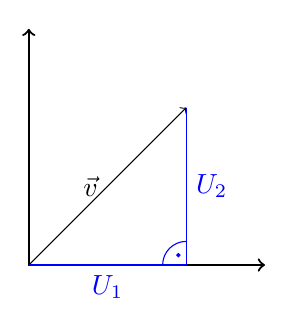
\begin{tikzpicture}
	\draw[thick, <->] (3,0) -- (0,0) -- (0,3);

	\draw[->] (0,0) -- (2,2) node[left, midway] {$\vec{v}$};
	\draw[draw=blue, thick] (0,0) -- (2,0) node[below, midway, text=blue] {$U_1$};
	\draw[draw=blue] (2,0) -- (2,2) node[right, midway, text=blue] {$U_2$};
	\draw[draw=blue] (1.7,0) arc (180:90:0.3);
	\draw[draw=blue, fill=blue] (1.9,0.125) circle (0.02);
\end{tikzpicture}\\
Pythagoras $\| \vec{u} \| = \sqrt{u_1^2 + u_2^2}$
\item Der Abstand zwischen zwei Punkten $A$ und $B$ (mit Ortsvektoren $\vec{a}$ bzw. $\vec{b}$ ist gleich der L�nge des Vektors $\vec{AB} = \vec{b} - \vec{a}$
		\[d\left(\vec{a}, \vec{b}\right) = \| \vec{b} - \vec{a} \| = \| \vec{a} - \vec{b} \|\]
\end{enumerate}}

\subsection{Orthogonalit�t}
\label{sec:6.6}
Zwei Vektoren $\vec{u}, \vec{v} \in \mathbb{R}^n$ nennt man orthogonal\index{orthogonal} bzw. senkrecht bzw. rechtwinklig wenn
\[\vec{u} \mal \vec{v} = 0\]
%15.01.2009-IMG-mathe-1
\begin{tikzpicture}
	\draw[<->, thick] (0,3) -- (0,0) node[left, midway] {$\vec{v}$} -- (5,0) node[below, midway] {$\vec{u}$};
	\draw[thick] (0,0.5) arc (90:0:0.5);
	\path (0,0) ++(45:0.25) node{$\alpha$};
\end{tikzpicture}

$\alpha = 90� \Ra \cosx{\alpha} = 0$

Man schreibt dann auch $\vec{u} \perp \vec{v}$.

\section{S�tze}
\subsection{Eigenschaften des Skalarproduktes}
\label{sec:6.2}
Seien $\vec{u}, \vec{v}, \vec{w} \in \mathbb{R}^n$, $\lambda \in \mathbb{R}$, dann gilt:
\begin{enumerate}[label=\roman*)]
\item Kommutativgesetz: $\vec{u} \mal \vec{v} = \vec{v} \mal \vec{u}$
\item Distributivgesetz: $\vec{u} \mal \left(\vec{v} + \vec{w}\right) = \vec{u} \mal \vec{v} + \vec{u} \mal \vec{w}$
\item $\left(\lambda \mal \vec{u}\right) \vec{v} = \lambda \mal \left(\vec{u} \mal \vec{v}\right) = \vec{u} \mal \left(\lambda \vec{v}\right)$
\item $\vec{u} \mal \vec{u} \geq 0$\\
		$\vec{u} \mal \vec{u} = 0 \Lra \vec{u} = \vec{0}$
\end{enumerate}
\bsp[nachrechnen]{Beweis:}

\subsection{Eigenschaften der Norm}
\label{sec:6.4}
Seien $\vec{u}, \vec{v} \in \mathbb{R}^n$, $\lambda \in \mathbb{R}$, dann gilt
\begin{enumerate}[label=\roman*)]
\item $\| \vec{u} \|^2 = \vec{u} \mal \vec{u}$
\item Homogenit�t: $\| \lambda \vec{u} \| = \left| \lambda \right| \mal \| \vec{u} \|$
\item $\| \vec{u} \| = 0 \Lra \vec{u} = 0$
\item Normierbarkeit: jedem Vektor $\vec{u} \neq \vec{0}$ kann ein normierter\index{Normierter} Vektor $\vec{v}$ zugewiesen werden mit $\vec{v} = \frac{1}{\| \vec{u} \|} \mal \vec{u}$ und $\| \vec{v} \| = 1$
\end{enumerate}
\bsp[nachrechnen]{Beweis:}

\subsection{Satz}
\label{sec:6.5}
Das Skalarprodukt zweier Vektoren $\vec{u}, \vec{v} \in \mathbb{R}^n$ kann man auch berechnen durch
\[\vec{u} \mal \vec{v} = \| \vec{u} \| \mal \| \vec{v} \| \mal \cosx{\alpha}\]
mit $\alpha$ als Winkel zwischen $\vec{u}$ und $\vec{v}$

%14.01.2009-IMG-mathe-2
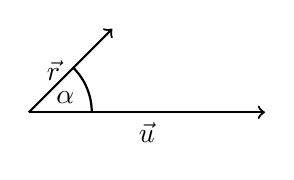
\begin{tikzpicture}
	\draw[->, thick] (0,0) -- (3,0) node[below, midway] {$\vec{u}$};
	\draw[->, thick] (0,0) -- (45:1.5) node[left, midway] {$\vec{r}$};
	\draw[thick] (0.8,0) arc (0:45:0.8);
	\path (0,0) ++(22.5:0.5) node{$\alpha$};
\end{tikzpicture}
%14.01.2009-IMG-mathe-3
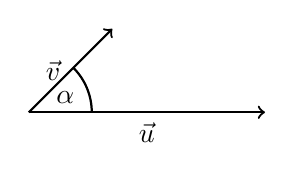
\begin{tikzpicture}
	\draw[->, thick] (0,0) -- (3,0) node[below, midway] {$\vec{u}$};
	\draw[->, thick] (0,0) -- (45:1.5) node[left, midway] {$\vec{v}$};
	\draw[thick] (0.8,0) arc (0:45:0.8);
	\path (0,0) ++(22.5:0.5) node{$\alpha$};
\end{tikzpicture}
%14.01.2009-IMG-mathe-4
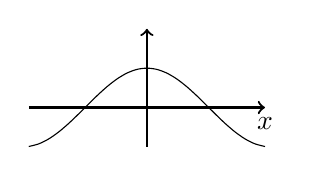
\begin{tikzpicture}
	\draw[->, thick] (-1.5,0) -- (1.5,0) node[below] {$x$};
	\draw[->, thick] (0,-0.5) -- (0,1);
	\draw[smooth] plot[domain=-3:3, scale=0.5] (\x,{cos(\x r)});
\end{tikzpicture}

\bsp[Winkel zwischen $\vec{u}$ und $\vec{v}$]{Beispiel:}{
Test Test Test
$\vec{u} \mal \vec{v} = \sumx{k = 1}{n}{u_k \mal v_k} = \| \vec{u} \| \mal \| \vec{v} \| \mal \cosx{\alpha}$\\
$\Lra \cosx{\alpha} = \frac{\vec{u} \mal \vec{v}}{\| \vec{u} \| \mal \| \vec{v} \|}$\\
$\Ra \alpha = \arccosx{\frac{\vec{u} \mal \vec{v}}{\| \vec{u} \| \mal \| \vec{v} \|}}$}

\subsection{Pythagoras}
\label{sec:6.7}
Seien $\vec{u}, \vec{v} \in \mathbb{R}^n$ dann gilt:
\[\vec{u} \perp \vec{v} \Lra \| \vec{u} + \vec{v} \| = \| \vec{u} \|^2 + \| \vec{v} \|^2\]
%15.01.2009-IMG-mathe-2
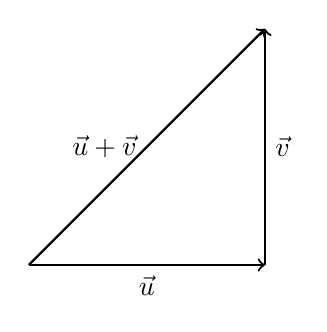
\begin{tikzpicture}
	\draw[->, thick] (0,0) -- (3,3) node[left, midway] {$\vec{u} + \vec{v}$};
	\draw[->, thick] (0,0) -- (3,0) node[below, midway] {$\vec{u}$};
	\draw[->, thick] (3,0) -- (3,3) node[right, midway] {$\vec{v}$};
\end{tikzpicture}

\bsp{Beweis:}{
\begin{align*}
	\| \vec{u} + \vec{v} \|^2 &= \left(\vec{u} + \vec{v}\right) \mal \left(\vec{u} + \vec{v}\right)\\
	&= \vec{u} \mal \left(\vec{u} + \vec{v}\right) + \vec{v} \mal \left(\vec{u} + \vec{v}\right)\\
	&= \vec{u} \mal \vec{u} + \vec{u} \mal \vec{v} + \vec{v} \mal \vec{u} + \vec{v} \mal \vec{v}\\
	&= \| \vec{u} \|^2 + \| \vec{v} \|^2 + 2 \underbrace{(\vec{u} \mal \vec{v})}_{= 0 \Lra \vec{u} \perp \vec{v}}\\
	&= \| \vec{u} \|^2 + \| \vec{v} \|^2
\end{align*}
%15.01.2009-IMG-mathe-3
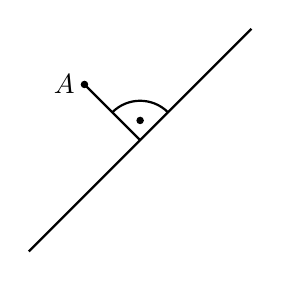
\begin{tikzpicture}
	\draw[thick] (0,0) -- (45:4);
	\draw[thick] (45:2) -- +(135:1);
	\draw[fill=black] (45:2) ++ (135:1) circle (0.04) node[left] {$A$};
	\draw[thick] (45:2) ++ (135:0.5) arc (135:45:0.5);
	\draw[fill=black] (45:2) ++ (90:0.25) circle (0.04);
\end{tikzpicture}
}

\section{Aufgaben}
\subsection{Aufgabe 5.1}
\label{sec:Aufgabe-EukVektorraum-A5.1}
Bestimmen sie die Menge $F$ aller Vektoren $\vec{v} \in \mathbb{R}^3$, f�r die gilt $\vec{v} \perp \vec{u} = \vektor{-1}{2}{3}$

L�sung siehe \vref{sec:Loesung-EukVektorraum-A5.1}.

\subsection{Aufgabe 5.2}
\label{sec:Aufgabe-EukVektorraum-A5.2}
Zeigen sie unter Verwendung des Skalarproduktes, dass das folgende Dreieck rechtwinklig ist:
\[A := \vektor{3}{-2}{12}, B := \vektor{7}{0}{11}, C := \vektor{6}{-7}{14}\]
L�sung siehe \vref{sec:Loesung-EukVektorraum-A5.2}.


\part{L�sungen, �bungs- und Erg�nzungsbl�tter}
\chapter{L�sungen}
\section{Mengen}
\subsection{Sportverein}
\label{sec:Loesung-Mengen-Sportverein}
L�sung zu Aufgabe \vref{sec:Aufgabe-Mengen-Sportverein}.

\begin{description}
	\item[$H$] ist die Menge aller Handballspieler
	\item[$F$] ist die Menge aller Fu�ballspieler
	\item[$E$] ist die Menge aller Eisl�ufer
	\item[$S$] ist die Menge aller Skifahrer
	\item[$V$] ist die Menge aller Vereinsmitglieder
\end{description}

Durch die Aufgabenstellung gilt das folgende:
\begin{itemize}
	\item $\emptyset=H\cap F$
	\item $E\subseteq F$
	\item $E\cup S=V$
\end{itemize}

Es gilt die Behauptung:\\
\qquad$H\subseteq S$

Es folgt der Beweis:
\begin{alignat*}{2}
&H = H\cap V &&=\\
&H\cap(E\cup S) &&=\\
&(H\cap E)\cup(H\cap S)\subseteq(H\cap F)\cup(H\cap S) &&=\\
&\emptyset\cup(H\cap S) &&=\\
&H\cap S\subseteq S
&\end{alignat*}

\subsection{Aufgabe 1}
\label{sec:Loesung-Mengen-AufgabeEins}
L�sung zu Aufgabe \vref{sec:Aufgabe-Mengen-AufgabeEins}.

\begin{enumerate}
\item TODO
\item TODO
\end{enumerate}

\subsection{Aufgabe 2}
\label{sec:Loesung-Mengen-AufgabeZwei}
L�sung zu Aufgabe \vref{sec:Aufgabe-Mengen-AufgabeZwei}.

\begin{multicols}{3}
\begin{enumerate}
	\item TODO
	\item TODO
	\item TODO
	\item TODO
	\item TODO
	\item TODO
\end{enumerate}
\end{multicols}
\renewcommand{\labelenumi}{\arabic{enumi}.}

\section{Logik}
\subsection{Aufgabe 1.2}
\label{sec:Loesung-Logik-AufgabeEinsPunktZwei}
L�sung zu Aufgabe \vref{sec:Aufgabe-Logik-AufgabeEinsPunktZwei}.

\begin{multicols}{3}
\renewcommand{\labelenumi}{zu \alph{enumi})}
\begin{enumerate}
\item $ $ \newline
		%TABL-09.10.2008-mathe-1
		\begin{tabular}{c|c||c}
		$A$ & $B$ & \\
		\hline
		$w$ & $w$ & $f$\\
		$w$ & $f$ & $f$\\
		$f$ & $w$ & $w$\\
		$f$ & $f$ & $f$\\
		\end{tabular}

\item $ $ \newline
		%TABL-09.10.2008-mathe-2
		\begin{tabular}{c|c||c}
		$A$ & $B$ & \\
		\hline
		$w$ & $w$ & $w$\\
		$w$ & $f$ & $f$\\
		$f$ & $w$ & $w$\\
		$f$ & $f$ & $w$\\
		\end{tabular}

\item $ $ \newline
		%TABL-09.10.2008-mathe-3
		\begin{tabular}{c|c||c}
		$A$ & $B$ & \\
		\hline
		$w$ & $w$ & $f$\\
		$w$ & $f$ & $w$\\
		$f$ & $w$ & $f$\\
		$f$ & $f$ & $f$\\
		\end{tabular}
\end{enumerate}
\end{multicols}

\subsection{Aufgabe 1.3}
\label{sec:Loesung-Logik-AufgabeEinsPunktDrei}
L�sung zu Aufgabe \vref{sec:Aufgabe-Logik-AufgabeEinsPunktDrei}.

\renewcommand{\labelenumi}{zu \alph{enumi})}
\begin{enumerate}
\item $A = 18$ ist durch $12$ teilbar\\
		$B = 18$ ist durch $3$ teilbar\\
		$A$ falsch, $B$ richtig $\Ra$ $A \Rightarrow B$ wahr
\item $A = 3$ ist Teiler von $8$\\
		$B = 14$ ist eine Primzahl\\
		$A$ falsch, $B$ falsch $\Ra$ $A \Leftrightarrow B$ wahr
\end{enumerate}
\renewcommand{\labelenumi}{\arabic{enumi}.}

\subsection{Aufgabe 6}
\label{sec:Loesung-Logik-AufgabeSechs}
L�sung zu Aufgabe \vref{sec:Aufgabe-Logik-AufgabeSechs}.

\renewcommand{\labelenumi}{zu \alph{enumi})}
\begin{enumerate}
\item $ $ \newline
		\begin{tabular}{c|c||c|c|c}
		$A$ & $B$ & $(\neg (A \und B))$ & $((\neg A) \oder B)$ & $(\neg (A \und B)) \und ((\neg A) \oder B)$
		\\\hline
		$w$ & $w$ & $f$ & $w$ & $f$
		\\$w$ & $f$ & $w$ & $f$ & $f$
		\\$f$ & $w$ & $w$ & $w$ & $w$
		\\$f$ & $f$ & $w$ & $w$ & $w$
		\end{tabular}
\item $ $ \newline
		\begin{tabular}{c|c||c}
		$A$ & $B$ & $((\neg A) \oder B) \Ra (A \und B)$
		\\\hline
		$w$ & $w$ & $w$
		\\$w$ & $f$ & $w$
		\\$f$ & $w$ & $f$
		\\$f$ & $f$ & $f$
		\end{tabular}
\end{enumerate}
\renewcommand{\labelenumi}{\arabic{enumi}.}

\subsection{Aufgabe 7}
\label{sec:Loesung-Logik-AufgabeSieben}
L�sung zu Aufgabe \vref{sec:Aufgabe-Logik-AufgabeSieben}.

\renewcommand{\labelenumi}{zu \alph{enumi})}
\begin{enumerate}
\item $ $ \newline
		\begin{tabular}{c|c|c||c|c|c}
		$A$ & $B$ & $C$ & $(A \oder B)$ & $\neg C$ & $(A \oder B) \Ra \neg C$
		\\\hline
		$w$ & $w$ & $w$ & $w$ & $f$ & $f$
		\\$w$ & $w$ & $f$ & $w$ & $w$ & $w$
		\\$w$ & $f$ & $w$ & $w$ & $f$ & $f$
		\\$w$ & $f$ & $f$ & $w$ & $w$ & $w$
		\\$f$ & $w$ & $w$ & $w$ & $f$ & $f$
		\\$f$ & $w$ & $f$ & $w$ & $w$ & $w$
		\\$f$ & $f$ & $w$ & $f$ & $f$ & $w$
		\\$f$ & $f$ & $f$ & $f$ & $w$ & $w$
		\end{tabular}
\item $ $ \newline
		\begin{tabular}{c|c|c||c|c|c}
		$A$ & $B$ & $C$ & $\neg A$ & $\neg B$ & $C \Ra (\neg A) \und (\neg B)$
		\\\hline
		$w$ & $w$ & $w$  & $f$ & $f$ & $w$  
		\\$w$ & $w$ & $f$ & $f$ & $f$ & $w$
		\\$w$ & $f$ & $w$ & $f$ & $w$ & $w$
		\\$w$ & $f$ & $f$ & $f$ & $w$ & $w$
		\\$f$ & $w$ & $w$ & $w$ & $f$ & $w$
		\\$f$ & $w$ & $f$ & $w$ & $f$ & $w$
		\\$f$ & $f$ & $w$ & $w$ & $w$ & $w$
		\\$f$ & $f$ & $f$ & $w$ & $w$ & $w$
		\end{tabular}
\end{enumerate}
\renewcommand{\labelenumi}{\arabic{enumi}.}

\subsection{Aufgabe 8}
\label{sec:Loesung-Logik-AufgabeAcht}
L�sung zu Aufgabe \vref{sec:Aufgabe-Logik-AufgabeAcht}.

$\begin{array}{rcl}
	F_1 &=& \neg A \und B\\
	F_2 &=& \neg B \und A\\
	F_3 &=& (\neg F_1) \und (\neg F_2)\\
	&=& (\neg(\neg A \und B)) \und (\neg(\neg B \und A))\\
	&=& (\neg(\neg A) \oder \neg B) \und (\neg(\neg B) \oder \neg A)\\
	&=& (A \oder \neg B) \und (B \oder \neg A)\\
	&=& (A \und B) \oder \neg (A \oder B)\\
	&=& (A \und B) \oder (\neg A \neg B)
\end{array}$

\subsection{Aufgabe 9}
\label{sec:Loesung-Logik-AufgabeNeun}
L�sung zu Aufgabe \vref{sec:Aufgabe-Logik-AufgabeNeun}

\subsubsection{Aufgaben L�sung}
\begin{tabular}{c|c|c|c||c|c|c}
$A$ & $B$ & $C$ & $D$ & $(A \oder B) \und D$ & $\overline{(A \oder B)} \und (C \oder D)$ & $C \Ra ((A \und D) \oder (B \und D))$
\\\hline
$f$ & $w$ & $f$ & $w$ & $w$ & $f$ & $w$\\
$w$ & $w$ & $w$ & $f$ & $f$ & $f$ & $f$\\
$f$ & $f$ & $f$ & $w$ & $f$ & $w$ & $w$
\end{tabular}

\subsection{Aufgabe 9}
\label{sec:Loesung-Logik-AufgabeZehn}
L�sung zu Aufgabe \vref{sec:Aufgabe-Logik-AufgabeZehn}

\renewcommand{\labelenumi}{zu \alph{enumi})}
\begin{enumerate}
\item $\forall x \in \mathbb{N}: x^2$ gerade\\
		$\neg (A x \in \mathbb{N}_0: x^2$ gerade\\
		$\aeq \exists x \in \mathbb{N}_0: x^2$ nicht gerade\\
		Es gibt mindestens eine ungerade Quadratzahl
\item $\exists n \in \mathbb{N}: n \notin \mathbb{Q}$\\
		$\neg (\exists n \in \mathbb{N}: n \notin \mathbb{Q})$\\
		$\aeq \forall n \in \mathbb{N}: n \in \mathbb{Q}$
\item $\neg((\forall$ Stra�en f�hren nach Rom) $\und$ ($\exists$ Pfad f�hrt nach Rom))\\
		$\aeq(\neq(\forall$ Stra�en f�hren nach Rom)) $\oder$ $(\neq (\exists$ Pfad f�hrt nach Rom))\\
		$\aeq(\exists$ Stra�e, die nicht nach Rom f�hrt) $\oder$ $(\forall$ Pfade f�hren nicht nach Rom)
\end{enumerate}
\renewcommand{\labelenumi}{\arabic{enumi}.}

\section{Relationen und Abbildungen}
\subsection{Aufgabe 1.4}
\label{sec:Loesung-RelationenUndAbbildungen-EinsPunktVier}
L�sung zu Aufgabe \vref{sec:Aufgabe-RelationenUndAbbildungen-EinsPunktVier}

\renewcommand{\labelenumi}{zu \alph{enumi})}
\begin{enumerate}
\item $R = $\gklamm{(1,1), (1,2), (1,3), (1,4), (3,1), (3,2), (3,3), (3,4)}
\item %TAB-15.10.2008-mathe-4
		\begin{minipage}{\textwidth}
		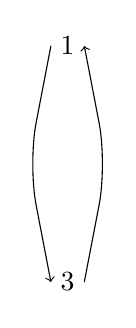
\begin{tikzpicture}
		%Nodes
		\node (Oben) 	at (0,0) 		{$1$};
		\node (Unten) 		at (0,-3) 		{$3$};

		%Verkn�pfungen
		\draw[->,rounded corners = 15pt] (Oben.west) -- (-0.5,-1.5) -- (Unten.west);
		\draw[->,rounded corners = 15pt] (Unten.east) -- (0.5,-1.5) -- (Oben.east);
		\end{tikzpicture}
		\end{minipage}
\item $\left(\begin{array}{cccc}
				 w & w & w & w\\
				 f & f & f & f\\
				 w & w & w & w\\
				 f & f & f & f
				 \end{array}\ \right)$
\end{enumerate}
\renewcommand{\labelenumi}{\arabic{enumi}.}

\subsection{Aufgabe 1.5}
\label{sec:Loesung-RelationenUndAbbildungen-EinsPunktFuenf}
L�sung zu Aufgabe \vref{sec:Aufgabe-RelationenUndAbbildungen-EinsPunktFuenf}

\begin{tabular}{r|c|c|c}
				& a 	& b 	& c\\
\hline
reflexiv		& x 	& 	& \\
\hline
symmetrisch	& x	& 	& \\
\hline
transitiv	& x 	& x	& x\\
\end{tabular}
\renewcommand{\labelenumi}{\arabic{enumi}.}

\section{Matrizen und Determinanten}
\subsection{Aufgabe 3.3}
\label{sec:Loesung-MatrizenundDeterminanten-Aufgabe-3-3}
L�sung zu Aufgabe \vref{sec:Aufgabe-MatrizenundDeterminanten-Aufgabe-3-3}
\begin{enumerate}
\item $A \mal B$
		\[= \varvektor{cc}{2 & -1\\1 & 0\\-3 & 4} \mal \varvektor{ccc}{1 & -2 & -5\\3 & 4 & 0} \in M(3, 3)\]
		\[= \varvektor{ccc}{2 - 3 & -4 - 4 & -10 + 0\\1 + 0 & -2 + 0 & -5 + 0\\-3 + 12 & 6 + 15 & 15 + 0} = \varvektor{ccc}{-1 & -8 & -10\\1 & -2 &-5\\9 & 22 & 15}\]

\item $B \mal A$
		\[= \varvektor{ccc}{1 & -2 & -5\\3 & 4 & 0} \mal \varvektor{cc}{2 & -1\\1 & 0\\-3 & 4} \in M(2, 2)\]
		\[= \varvektor{cc}{2 - 2 + 15 & -1 + 0 -20\\6 + 4 + 0 & -3 + 0 + 0} = \varvektor{cc}{15 & -21\\10 & -3}\]

\item $C \mal D$
		\[= \varvektor{cc}{1 & 6\\-3 & 5} \mal \varvektor{cc}{4 & 0\\2 & -1} = \varvektor{cc}{4 + 12 & 0 - 6\\-12 + 10 & 0 - 5} = \varvektor{cc}{16 & -6\\-2 & -5}\]

\item $D \mal C$
		\[= \varvektor{cc}{4 & 0\\2 & -1} \mal \varvektor{cc}{1 & 6\\-3 & 5} = \varvektor{cc}{4 + 0 & 24 + 0\\2 + 3 & 12 - 5} = \varvektor{cc}{4 & 24\\5 & 7}\]
\end{enumerate}

\section{Vollst�ndige Induktion}
\subsection{Aufgabe A16}
\label{sec:Loesung-VollstaendigeInduktion-A16}
L�sung zu Aufgabe \vref{sec:Aufgabe-VollstaendigeInduktion-A16}

Induktionsschluss von $n = 1$ auf $n +1 = 2$ ist falsch, denn die beiden einelementigen Teilmengen haben keine Schnittmenge $\neq \emptyset$.

\section{Vektorraum}
\subsection{Aufgabe 4.5}
\label{sec:Loesung-Vektorraum-A4.5}
L�sung zu Aufgabe \vref{sec:Aufgabe-Vektorraum-A4.5}
\[A^2 = \varvektor{rrr}{4 & -6 & 6\\3 & -5 & 6\\3 & -6 & 7}\]
\[B = \gklamm{\varvektor{ccc}{1 & 0 & 0\\0 & 0 & 0\\0 & 0 & 0}, \varvektor{ccc}{0 & 1 & 0\\0 & 0 & 0\\0 & 0 & 0}, \dots, \varvektor{ccc}{0 & 0 & 0\\0 & 0 & 0\\0 & 1 & 0}, \varvektor{ccc}{0 & 0 & 0\\0 & 0 & 0\\0 & 0 & 1}}\]
\[(A)_B = \varvektor{c}{2\\-6\\6\\3\\-7\\6\\3\\-6\\5}, (A^2)_B = \varvektor{c}{4\\-6\\6\\3\\-5\\6\\3\\-6\\7}, (E_3)_B = \varvektor{c}{1\\0\\0\\0\\1\\0\\0\\0\\1}\]
\[\gauss{ccc|c}{2 & 4 & 1 & 0\\\vdots & \vdots & \vdots & \vdots\\5 & 7 & 1 & 0} \ra \gauss{ccc|c}{2 & 4 & 1 & 0\\3 & 3 & 0 & 0\\-7 & 5 & 1 & 0\\5 & 7 & 1 & 0} \ra \gauss{ccc|c}{2 & 4 & 1 & 0\\3 & 3 & 0 & 0}\]
\[\ra \gauss{ccc|c}{2 & 4 & 1 & 0\\0 & -3 & 1 \frac{1}{2} & 0}\]
$\Ra$ $A$, $A^2$, $E_3$ sind linear abh�ngig

\subsection{Aufgabe 4.7}
\label{sec:Loesung-Vektorraum-A4.7}
L�sung zu Aufgabe \vref{sec:Aufgabe-Vektorraum-A4.7}
\begin{align*}
	\varvektor{rr}{1 & -2\\3 & 4} &= x_1 \varvektor{cc}{0 & 1\\1 & 0} + x_2 \varvektor{cc}{0 & -1\\0 & 0} + x_3 \varvektor{cc}{1 & -1\\0 & 3} + x_4 \varvektor{cc}{0 & 1\\0 & 1}\\
	&\Leftrightarrow \varvektor{c}{1\\-2\\3\\4} = x_1 \varvektor{c}{0\\1\\1\\0} + x_2 \varvektor{c}{0\\-1\\0\\0} + x_3 \varvektor{c}{1\\-1\\0\\3} + x_4 \varvektor{c}{0\\1\\0\\1}\\
	&\Leftrightarrow \gauss{rrrr|r}{0 & 0 & 1 & 0 & 1\\1 & -1 & -1 & 1 & -2\\1 & 0 & 0 & 0 & 3\\0 & 0 & 3 & 1 & 4} \underrightarrow{\RM{1} \leftrightarrow \RM{3}}\\
	&\underrightarrow{\RM{2} = \RM{2} (-1)}_{\RM{4} = \RM{4} - 3 \RM{2}}\\
	&\underrightarrow{\RM{2} = \RM{2} + \RM{4}}\\
	&\underrightarrow{\RM{2} = \RM{2} - \RM{3}}\\
	\varvektor{rr}{1 & -2\\3 & 4}_{\mathcal{B}} = \varvektor{c}{3\\5\\1\\1}
\end{align*}

\subsection{Aufgabe 4.8}
\label{sec:Loesung-Vektorraum-A4.8}
L�sung zu Aufgabe \vref{sec:Aufgabe-Vektorraum-A4.8}
\begin{enumerate}[label=\alph*)]
\item $\vektor{3}{-5}{4} = x_1 \vektor{1}{0}{0} + x_2 \vektor{1}{1}{0} + x_3 \vektor{1}{1}{1}$\\
		$\gauss{ccc|c}{1 & 1 & 1 & 3\\0 & 1 & 1 & -5\\0 & 0 & 1 & 4} \underrightarrow{\RM{1} = \RM{1} - \RM{2}}$\\
		$\underrightarrow{\RM{2} = \RM{2} - \RM{3}}$\\
		$\Ra \vec{U}_{\mathcal{B}} = \vektor{8}{-9}{4}$

\item $\vec{v} = -4 \mal \vektor{1}{0}{0} + 8 \vektor{1}{1}{0} - 7 \vektor{1}{1}{1} = \vektor{-4 + 8 - 7}{0 + 8 - 7}{0 + 0 - 7} = \vektor{-3}{1}{-7}$
\end{enumerate}

\section{Euklidischer Vektorraum $\mathbb{R}^n$}
\subsection{Aufgabe 5.1}
\label{sec:Loesung-EukVektorraum-A5.1}
L�sung zu Aufgabe \vref{sec:Aufgabe-EukVektorraum-A5.1}
\[\vec{v} = \vektor{a}{b}{c}, \vec{u} = \vektor{-1}{2}{3}\]
\[\vec{v} \mal \vec{u} = -a + 2b + 3c = 0\]
\begin{align*}
	F &= \gklamm{\vektor{a}{b}{c} \in \mathbb{R}^3 \vert -a + 2b + 3c = 0, a, b, c \in \mathbb{R}}\\
	&= \gklamm{\underbrace{\vektor{2b + 3c}{b}{c}}_{b \mal \vektor{2}{1}{0} + c \mal \vektor{3}{0}{1}} \in \mathbb{R}^3 \vert b, c \in \mathbb{R}}
\end{align*}
\subsection{Aufgabe 5.2}
\label{sec:Loesung-EukVektorraum-A5.2}
L�sung zu Aufgabe \vref{sec:Aufgabe-EukVektorraum-A5.2}
\[\vec{AB} = -(\vec{b} - \vec{a}) = \vektor{-(7 - 3)}{-(0 - (-2))}{-(11 - 12)} = \vektor{-4}{-2}{1}\]
\[\vec{AC} = -(\vec{c} - \vec{a}) = \vektor{-3}{5}{-2}\]
\[\vec{AB} \mal \vec{AC} = \alpha\]
\[\vec{AB} \mal \vec{AC} = 12 - 10 - 2 = 0 \Ra \alpha = 90�\]

\chapter{�bungsbl�tter}
\section{L�sungen}
\subsection{�bung 1.1}
\label{sec:Uebungsblaetter_1_1L}
%L�sung zu Aufgabe \vref{sec:Uebungsblaetter_1_1}.

\begin{itemize}
\item 3 Wagen 1. Klasse
\item 5 Wagen 2. Klasse
\item 2 Gep�ckwagen
\end{itemize}

\begin{enumerate}[label=\alph*)]
\item $\binom{10}{3} \mal \binom{7}{5} \mal \binom{2}{2} = \frac{10 \mal 9 \mal 8}{3!} \mal \frac{7 \mal 6 \mal 5 \mal 4 \mal 3}{5!} \mal \frac{2 \mal 1}{2!} = \frac{10!}{3! \mal 5! \mal 2!}$\\
		$\binom{10}{3}$: Anzahl m�glicher Pl�tze f�r 1. Klasse auszusuchen\\
		$\binom{7}{5}$: Anzahl M�glichkeiten im Anschluss Pl�tze f�r 2. Klasse festzulegen\\
		$\binom{2}{2}$: Letzte 2 Pl�tze im Gep�ckwagen

\item Wagen wie in a), alle 2. Klasse Wagen am St�ck

		%MA-02.04.2009-IMG-1
		\begin{tikzpicture}[decoration=brace]
		\draw[thick, ->] (0,0) -- (6,0) node[below] {$n$};
		\draw[-|] (2,-0.2) node[below] {$n - 1$} -- (2,1.8) node[left]{$S_{n - 1}$};
		\draw[-|] (3,-0.2) node[below] {$n$} -- (3,2.8) node[above]{$S_1$};
		\draw[dashed] (2,1.8) -- (5,1.8);
		\draw[dashed] (3,2.8) -- (5,2.8);
		\draw[decorate] (2.5,2.8) -- (2.5,1.8) node[right, midway] {$\epsilon$};
		\draw (3,2.8) -- (2.5,2.8);
		
		\draw[draw=red, <->] (5,2.8) node[right] {$S$} -- (5,1.8) node[right,midway] {$> \frac{\epsilon}{2}$};
		\draw[draw=blue, <->] (6,0) node[right] {$S$} -- (6,2.8) node[right,midway] {$> \frac{\epsilon}{2}$};
		\end{tikzpicture}

		6 M�glichkeiten den Platz des ersten 2. Klasse Wagens festzulegen\\
		$\binom{5}{3} \mal \binom{2}{2}$ Anzahl M�glichkeiten die Pl�tze f�r die anderen Wagen festzulegen\\
		$6 \mal \binom{5}{3} \mal \binom{2}{2} = 6 \mal \frac{5 \mal 4 \mal 3}{1 \mal 2 \mal 3} = 60$
\end{enumerate}

\subsection{�bung 1.2 (Abwandlung)}
\label{sec:Uebungsblaetter_1_2AL}
%L�sung zu Aufgabe \vref{sec:Uebungsblaetter_1_2A}.

\begin{itemize}
\item 12 stellige Zahl mit Ziffern 1-9
\item max zwei 9
\item Summe der ersten beiden 16
\end{itemize}

\subsubsection*{ersten beiden Stellen}
$\left.88\right\}$ \textcircled{1}\\
$\left.\begin{array}{l}
79\\
97
\end{array}\right\}$ \textcircled{2}

\begin{enumerate}[label=\textcircled{\arabic*}]
\item M�glichkeiten noch $2 \times 9$, $1 \times 9$, $0 \times 9$ in den 10 Stellen\\
		$\binom{10}{2} \mal 8 + \binom{10}{1} \mal 8^9 + \binom{10}{0} \mal 8^{10}$\\
		$8$ ist die Anzahl der M�glichkeiten pro Stelle\\
		$\space^8$ ist die Anzahl der Stellen

\item M�glichkeiten noch $1 \times 9$ oder $0 \times 9$ in 10 Stellen\\
		$\binom{10}{1} \mal 8^9 + \binom{10}{0} \mal 8^{10}$\\
		\Ra Totale Anzahl = $1 \mal \rkl{\rkl{\binom{10}{2} \mal 8^8 + \binom{10}{1} \mal 8^9 + \binom{10}{0} \mal 8^{10}} + 2 \mal \rkl{\binom{10}{1} \mal 8^9 + \binom{10}{0} \mal 8^{10}}}$
\item 
\end{enumerate}

\subsection{�bung 1.3}
\label{sec:Uebungsblaetter_1_3L}
%L�sung zu Aufgabe \vref{sec:Uebungsblaetter_1_3}.

zu zeigen $\forall n \in \N_0: \sum_{k = 0}^n \binom{m + k}{k} = \binom{m + n + 1}{n}$
\begin{description}
\item[(IA)] $n = 0$
		\[\left.\begin{array}{l}
		\tx{LS} = \sum_{k = 0}^0 \binom{m + k}{k} = \binom{m + 0}{0} = 1\\
		\tx{RS} = \binom{m + 0 + 1}{0} = 1
		\end{array}\right\} \checkmark\]

\item[(IS)] zu zeigen $\forall n \in \N: \underbrace{\sum_{k = 0}^n \binom{m + k}{k} = \binom{m + n + 1}{n}}_{= \tx{(IV)}}$ \Ra $\sum_{k = 0}^{n + 1} \binom{m + k}{k} = \binom{m + n + 2}{n + 1}$
		\begin{align*}
		&\sum_{k = 0}^{n + 1} \binom{m + k}{k} = \binom{m + n + 1}{n + 1} + \sum_{k = 0}^n \binom{m + k}{k}\\
		\stack{=}{\tx{(IV)}} & \underbrace{\binom{m + n + 1}{n + 1}}_{\binom{m + n + 1}{m}} + \binom{m + n + 1}{n} \underbrace{=}_{\tx{Satz 1.3 iii)}} \binom{m + n + 2}{n + 1}
		\end{align*}\qed
\end{description}

\subsection{�bung 1.4}
\label{sec:Uebungsblaetter_1_4L}
%L�sung zu Aufgabe \vref{sec:Uebungsblaetter_1_4}.

F�r welche $(x, y) \in \mb{R}^2$ gilt:
\[xy \klgl x^2 + y^2\]
\textit{Behauptung:} Gilt f�r alle $(x, y) \in \mb{R}^2$
\begin{description}
\item[Fall 1] $xy \klgl 0$ (\ac{d.h.} $(x \klgl 0 \und y \grgl 0) \oder (x \klgl 0 \und y \grgl 0)$\\
		\begin{align*}
		&x y \klgl 0 \tx{ und } \underbrace{x^2}_{\grgl 0} + \underbrace{y^2}_{\grgl 0} \grgl 0\\
		\Ra &xy \klgl x^2 + y^2
		\end{align*}

\item[Fall 2] $xy > 0 (\Lra (x > 0 \und y > 0) \oder (x < 0 \und y < 0)$
		\begin{align*}
		&xy \stack{\klgl}{!} x^2 + y^2~~~~\vert - xy\\
		\Lra &0 \stack{\klgl}{!} x^2 - xy + y^2
		\La &x^2 - xy + y^2 > x^2 - x - \underbrace{xy}_{> 0} + y^2 = (x - y)^2 \grgl 0
		\end{align*}\qed
\end{description}

\subsection{�bung 1.5}
\label{sec:Uebungsblaetter_1_5L}
%L�sung zu Aufgabe \vref{sec:Uebungsblaetter_1_5}.

$\betrag{\frac{3 - 2x}{2 + x}} \klgl 4$ $x \in \mb{R} \backslash \gklamm{-1}$\\
\Lra $-4 \klgl \frac{3 - 2x}{1 + x} \klgl 4$
\begin{description}
\item[Fall 1] $1 + x > 0 (\Lra x > - 1)$
		\begin{align*}
		\Lra &-4(1 + x) \klgl 3 - 2x \klgl 4(1 + x)\\
		\Lra &-4 -4x \klgl 3 - 2x \klgl 4 + 4x\\
		\Lra &\matrixp{-4 -4x \klgl 3 - 2x \vert + 4x - 3\\\Lra - 7 \klgl 2x \vert : 2\\\Lra -\frac{7}{2} \klgl x} \und \matrixp{3 - 2x \klgl 4 + 4x \vert +2x - 4\\- 1 \klgl 6x \vert :6\\-\frac{1}{6} \klgl x}\\
		&L_1 = \left[- \frac{1}{6}, \infty\right)
		\end{align*}

\item[Fall 2] $1 + x < 0$ ($\Lra x < - 1$)
		\begin{align*}
		\Lra &-4(1 + x) \grgl 3 - 2x \grgl 4(1 + x)\\
		\Lra &-4 -4x \grgl 3 - 2x \grgl 4 + 4x\\
		\Lra &\matrixp{-4 -4x \grgl 3 - 2x \vert + 4x - 3\\\Lra - 7 \grgl 2x \vert : 2\\\Lra -\frac{7}{2} \grgl x} \und \matrixp{3 - 2x \grgl 4 + 4x \vert +2x - 4\\- 1 \grgl 6x \vert :6\\-\frac{1}{6} \grgl x}\\
		&L_2 = \left(\infty, -\frac{7}{2}\right]
		\end{align*}
\end{description}
\[L = L_1 \cup L_2 ) \left(-\infty, -\frac{7}{2}\right] \cup \left[-\frac{1}{6}, \infty\right)\]

\subsection{�bung 2.1}
$a_{n + 1} = \frac{1}{2} \rkl{a_n + \frac{x_0}{a_n}} ~~ n \in \N$
\begin{enumerate}[label=\alph*)]
\item \ac{z.z.} $a_n > \sqrt{x_0}$
		\begin{description}
		\item[(IA)] $n = 1$ $a_1 > \sqrt{x_0}$ erf�llt nach Voraussetzung
		\item[(IS)] \ac{z.z.} $a_n > \sqrt{x_0} \Ra a_{n + 1} > \sqrt{x_0}$
				\begin{align*}
				a_{n + 1} &= \frac{1}{2} \rkl{a_n + \frac{x_0}{a_n}} = \ub{\frac{1}{2a_n}}{> 0} \rkl{a_n^2 + x_0}\\
				&= \frac{1}{2a_n} \rkl{a_n^2 - 2a_n \sqrt{x_0} + \rkl{\sqrt{x_0}}^2 + 2a_n \mal \sqrt{x_0}}\\
				&= \frac{1}{2a_n} \rkl{a_n^2 - 2a_n \sqrt{x_0} + \rkl{\sqrt{x_0}}^2} + \sqrt{x_0}\\
				&= \ub{\frac{1}{2a_n}}{>0} \ub{\rkl{\ub{a_n - \sqrt{x_0}}{> 0}}^2} + \sqrt{x_0} > \sqrt{x_0}\\
				\Ra& (a_n)_{n \in \N} \tx{ monoton fallend}
				\end{align*}
		\end{description}

\item \ac{z.z.} $(a_n)_{n \in \N}$ monoton fallend
		\begin{align*}
		a_{n + 1} - a_n &= \frac{1}{2} \rkl{a_n + \frac{x_0}{a_n}} - a_n = \frac{x_0}{2a_n} - \frac{1}{2} a_n\\
		&= \frac{x_0 - a_n^2}{2a_n} = \ub{\frac{1}{2a_n}}{>0} \ub{\rkl{\sqrt{x_0} - a_n}}{<0} \mal \ub{\rkl{\sqrt{x_0} + a_n}}{>0} < 0
		\end{align*}

\item \ac{z.z.} $\lim_{n \ra \infty} a_n = \sqrt{x_0}$
		\begin{align*}
		&a = \lim_{n \ra \un} a_n = \lim_{n \ra \un} a_n + 1 = \lim_{n \ra \un} \rac{1}{2} \rkl{a_n + \frac{x_0}{a_n}} = \frac{1}{2} \rkl{a + \frac{x_0}{a}}\\
		\Lra& \rac{1}{2} a = \frac{x_0}{2a} \Vert a \mal 2\\
		\Lra& a^2 = x_0\\
		\stack{a > 0}{\Lra}& a = \sqrt{x_0}
		\end{align*}

\item $a_1 = 2$, $x_0 = 2$\\
		\[a_2 = \frac{1}{2} \rkl{a_1 + \frac{2}{a_1}} = \frac{1}{2} \rkl{2 + \frac{2}{2}} = \frac{3}{2}\]
		\[a_3 = \frac{1}{2} \rkl{a_2 + \rac{2}{a_2}} = \frac{1}{2} \rkl{\frac{3}{2} + \rac{2 \mal 2}{3}} = \rac{9 + 8}{2 \mal 6} = \frac{17}{12}\]
		\begin{align*}
		\betrag{a - \sqrt{2}} &= a_3 - \sqrt{2} = \frac{a_3^2 - 2}{a_3 + \sqrt{2}} \klgl \frac{a_3^2 - 2}{a_3}\\
		&= a_3 - \frac{2}{a_3} = \frac{17}{12} - \frac{2 \mal 12}{17} = \frac{289 - 288}{12 \mal 17} = \frac{1}{12 \mal 17}\\
		\Ra& \sqrt{2} \in \eklamm{\ub{\frac{17}{12}}{a_3} - \frac{1}{12 \mal 17}, \ub{\frac{17}{12}}{a_3}}
		\end{align*}
\end{enumerate}

\subsection{�bung 2.2}
\begin{enumerate}[label=\alph*)]
\item $a_n = n - \sqrt{n^2 - b}$
		\begin{align*}
		\lim_{n \ra \un} a_n &= \frac{\rkl{n - \sqrt{n^2 - 5n}} \mal \rkl{n + \sqrt{n^2 - 5n}}}{n + \sqrt{n^2 - 5n}}\\
		&= \lim_{n \ra \un} \frac{n^2 - \rkl{n^2 - 5n}}{n + \sqrt{n^2 - 5n}} = \lim_{n \ra \un} \frac{5n}{n + \sqrt{n^2 - 5n}}\\
		&= \lim_{n \ra \un} \frac{5}{1 + \sqrt{\frac{n^2}{n^2} - \frac{5n}{n^2}}} = \lim_{n \ra \un} \frac{5}{1 + \sqrt{1 - \frac{5}{n}}} = \frac{5}{2}
		\end{align*}

\item $b_n = \frac{\sinx{n}}{n}$
		\begin{align*}
		0 &\klgl \lim_{n \ra \un} \betrag{b_n} = \lim_{n \ra \un} \betrag{\frac{\sinx{n}}{n}} \klgl \lim_{n \ra \un} \frac{1}{n} = 0\\
		&\Ra \lim_{n \ra \un} b_n = 0
		\end{align*}

\item $c_n = n \rkl{1 - \rkl{1 - \frac{1}{n}}^{42}}$
		\begin{align*}
		\lim_{n \ra \un} n \rkl{1 - \rkl{1 - \frac{1}{n}}^{42}} &= \lim_{n \ra \un} n \rkl{1 - \sum_{k = 0}^{42} \binom{42}{k} \rkl{-\frac{1}{n}}^k}\\
		&= \lim_{n \ra \un} n \rkl{\sum_{k = 1}^{42} \binom{42}{k} \mal \rkl{-1}^{k - 1} \rkl{\frac{1}{n}}^k}\\
		&= \lim_{n \ra \un} \sum_{k = 1}^{42} \binom{42}{k} \mal \rkl{-1}^{k - 1} \rkl{\frac{1}{n}}^{k - 1}\\
		&= \binom{42}{1} + \sum_{k = 2}^{42} \mal (-1)^{k - 1} \mal \rkl{\ub{\lim_{n \ra \un} \rkl{\frac{1}{n}}}{=0}}^{k - 1} = \binom{42}{1} = 42
		\end{align*}

\item $d_n = \rkl{1 + \frac{1}{n}}^{n^2}$\\
		Behauptung: $(d_n)_{n \in \N}$ ist divergent (genauer $\lim_{n \ra \un} d_n = \un$)
		\begin{align*}
		&\rkl{1 + \frac{1}{2}}^{n^2} = \rkl{\rkl{1 + \frac{1}{n}}^n}^n \ub{\grgl}{\tx{f�r $n$ gen�gend gro�}} \rkl{\ub{\rkl{1 + \frac{1}{n}}^n}{\overrightarrow{n \ra \un} e}}^k\\
		\Ra& \lim_{n \ra \un} \rkl{1 + \frac{1}{n}}^{n^2} \ub{\grgl}{\tx{f�r $\forall k \in \N$}} \rkl{\lim_{n \ra \un} \rkl{1 + \frac{1}{n}}^n}^k = e^k\\
		&\forall K \in \R \exists k \in \N:~e^k > K
		\end{align*}
		\Ra $(d_n)$ ist nicht nach oben beschr�nkt und damit divergent

\item $e_n = \sqrt[n]{\sqrt[n]{n!}}$
		\begin{align*}
		&\lim_{n \ra \un} e_n = \lim_{n \ra \un} \sqrt[n]{\sqrt[n]{n!}} = \tx{\textcircled{$\star$}}\\
		&\tx{\textcircled{$\star$}} \grgl \lim_{n \ra \un} \sqrt[n]{\sqrt[n]{1}}  = \lim_{n \ra \un} \sqrt[n]{1} = 1\\
		&\tx{\textcircled{$\star$}} \klgl \lim_{n \ra \un} \sqrt[n]{\sqrt[n]{n^n}} = \lim_{n \ra \un} \sqrt[n]{n} = 1\\
		\Ra& \lim_{n \ra \un} \sqrt[n]{\sqrt[n]{n!}} = 1
		\end{align*}
\end{enumerate}

\subsection{�bung 2.3}
\begin{enumerate}[label=\alph*)]
\item gesucht $p, q \in \N$ mit $\frac{p}{qq} = 0,\overline{4711}$
		\begin{align*}
		0,\overline{4711} &= \frac{4711}{10^4} + \frac{4711}{10^8} + \frac{4711}{10^{12}} + \dots\\
		&= 4711 \sum_{k = 1}^{\un} \rkl{\frac{1}{10^4}}^k = 4711 \frac{1}{10^4} \sum_{k = 0}^{\un} \rkl{\frac{1}{10^4}}^k\\
		&= 4711 \frac{1}{10^4} \mal \frac{1}{1 - \frac{1}{10^4}} = 4711 \mal \frac{1}{10^4 - 1}\\
		&= \frac{4711}{9999} \Ra p = 4711, q = 9999
		\end{align*}

\item $\frac{p}{q} = 0,1230\overline{443}$
		\begin{align*}
		\frac{p}{q} &= 0,1230\overline{443} = \frac{123}{1000} + \frac{443}{10^7} + \frac{443}{10^{10}} + \frac{443}{10^{13}} + \dots\\
		&= \frac{123}{10^3} + \frac{443}{10^7} \sum_{k = 0}^{\un} \rkl{\frac{1}{10^3}}^k = \frac{123}{10^3} + \frac{443}{10^7} \mal \frac{1}{1 - \frac{1}{10^3}}\\
		&= \frac{123}{10^3} + \frac{443}{10^4} \mal \frac{1}{999} = \frac{123 \mal 9990 + 443}{9990000}\\
		&= \frac{1229213}{9990000}
		\end{align*}
\end{enumerate}

\subsection{�bung 2.4}
$a_n = $ In der $n$-ten Minute zur�ckgelegte Anteil am Gummiband\\
$a_1 = \frac{25cm}{100cm} = \frac{1}{4}$\\
$a_2 = \frac{25cm}{200cm} = \frac{1}{8}$\\
$a_3 = \frac{25cm}{300cm} = \frac{1}{12}$\\
$a_n = \frac{1}{4n}$
bis und mit $n$-ter Minute zur�ckgelegter Anteil
\[\sum_{n = 1}^{N} a_n = \sum_{n = 1}^{N} \frac{1}{4n} = \frac{1}{4} \ub{\sum_{n = 1}^{N} \frac{1}{n}}{\tx{harmonische Reihe}}\]
\Ra die Ameise erreicht das Ende
\[\frac{1}{4} \sum_{n = 1}^{N} \frac{1}{n} \grgl 1\]
kleinstes $N$, welches die Bedingung erf�llt\\
\Ra $N = 31min$

\subsection{�bung 2.5}
\begin{enumerate}[label=\alph*)]
\item $\sum_{h = 0}^{\un} \frac{m!}{m^m}$ konvergent oder divergent?\\
		Majorantenkriterium
		\[
		\sum_{m = 0}^{\un} \frac{m!}{m^m} = \sum_{m = 0}^{\un} \rkl{\ub{\frac{m}{m}}{=1} \mal \ub{\frac{(m - 1)}{m}}{<1} \mal \ub{\frac{3}{m}}{<1} \mal \frac{2}{m} \mal \frac{1}{m}} \klgl 1 + \ub{2 \mal \sum_{m = 1}^{\un} \frac{1}{m^2}}{\tx{konvergent}}
		\]

\item $\sum_{h = 0}^{\un} \frac{m!}{m^m}$ konvergent oder divergent?\\
		notwendiges Kriterium 
		\[
		\sum_{m = 0}^{\un} \frac{m!}{m^m} = \sum_{m = 0}^{\un} \rkl{\ub{\frac{m}{m}}{=1} \mal \ub{\frac{(m - 1)}{m}}{<1} \mal \ub{\frac{3}{m}}{<1} \mal \frac{2}{m} \mal \frac{1}{m}} \klgl 1 + \ub{2 \mal \sum_{m = 1}^{\un} \frac{1}{m^2}}{\tx{konvergent}}
		\]

\item $\sum_{n = 1}^{\infty} \frac{\sinx{n}}{n^2}$ konvergent/divergent?\\
		Majorantenkriterium
		\[\betrag{\sum_{n = 1}^{\un} \frac{\sinx{x}}{n^2}} \klgl \sum_{n = 1}^{\un} \betrag{\frac{\sinx{n}}{n^2}} \klgl \sum_{n = 1}^{\un} \frac{1}{n^2}\]
		verallgemeinerte harmonische Reihe mit\\
		$\alpha = 2$ \Ra konvergent
\end{enumerate}

\subsection{�bung 2.6}
\begin{enumerate}[label=\alph*)]
\item $\sum_{n = 0}^{\un} \ub{\rkl{\frac{1}{2^n} + \frac{1}{3^n}}}{= a_n} \rkl{x - \ub{0}{= x_0}}^n$\\
		Quotientenmethode
		\begin{align*}
		\lim_{n \ra \un} \betrag{\frac{a_n}{a_{n + 1}}} &= \lim_{n \ra \un} \rkl{\rkl{\frac{1}{2^n}} + \frac{1}{3^n}} \mal \rkl{\frac{1}{2^{n + 1}} + \frac{1}{3^{n + 1}}^{-1}}\\
		&= \lim_{n \ra \un} \frac{\frac{1}{2^n} + \frac{1}{3^n}}{\frac{1}{2^{n + 1}} + \frac{1}{3^{n + 1}}} = \lim_{n \ra \un} \frac{\frac{3^n + 2^n}{6^n}}{\frac{3^{n + 1} + 2^{n + 1}}{6^{n + 1}}} = \lim_{n \ra \un} \frac{\rkl{3^n + 2^n} \mal 6^{n + 1}}{6^n \rkl{3^{n + 1} + 2^{n + 1}}}\\
		&= 6 \mal \lim_{n \ra \un} \frac{3^n + 2^n}{3^{n + 1} + 2^{n + 1}} = 6 \mal \lim_{n \ra \un} \frac{1 + \rkl{\frac{2}{3}}^n}{3 + 2 \mal \rkl{\frac{2}{3}}^n}\\
		&= 6 \mal \frac{lim_{n \ra \un} \rkl{1+ \rkl{\frac{2}{3}}^n}}{\lim_{n \ra \un} \rkl{3 + 2 \rkl{\frac{2}{3}}^n}} = 6 \mal \frac{1}{3} = 2
		\end{align*}
		Konvergenzradius $r = q = 2$

\item $\sum_{k = 0}^{\un} \frac{\rkl{2k}!}{\rkl{k!}^k} \rkl{x + 2}^k = \sum_{k = 0}^{\un} \ub{\frac{\rkl{2k}!}{\rkl{k!}^k}}{=a_k} \mal \rkl{x - \ub{\rkl{-2}}{= x_0}}^k$\\
		Wurzelmethode
		\begin{align*}
		0 \klgl \lim_{k \ra \un} \sqrt[k]{\betrag{a_k}} &= \lim_{k \ra \un} \sqrt[k]{\betrag{\frac{(2k)!}{(k!)^k}}} = \lim_{k \ra \un} \sqrt[k]{(2k)!} \mal \frac{1}{\sqrt[k]{k!^k}}\\
		&= \lim_{k \ra \un} \frac{1}{k!} \mal \sqrt[k]{(2k)!} \klgl \lim_{k \ra \un} \frac{1}{k!} \sqrt[k]{(2k)^{2k}} = \lim_{k \ra \un} \frac{(2k)^2}{k!} = 0
		\end{align*}
		\Ra Konvergenzradius $r = \un$
\item 
\item 

\end{enumerate}

\chapter{Erg�nzungsbl�tter}
\section{Erg�nzungsblatt 03}
\subsection{Aufgabe 12}

\subsection{Aufgabe 13}
\subsubsection{L�sung}
\renewcommand{\labelenumi}{\alph{enumi})}
\begin{enumerate}
\item 
\item 
\end{enumerate}
\renewcommand{\labelenumi}{\arabic{enumi}.}

\subsection{Aufgabe 14}

\subsection{Aufgabe 15}

\subsection{Aufgabe 16}

\subsection{Aufgabe 17}
\subsubsection{Aufgabenstellung}
Seien $A, B$ beliebige Mengen, Beweisen oder widerlegen sie die folgenden Aussagen:
\renewcommand{\labelenumi}{\alph{enumi})}
\begin{enumerate}
\item $\mathscr{P}(A \cup B) \subseteq (\mathscr{P}(A) \cup \mathscr{P}(B))$
\item $\mathscr{P}(A \cup B) = (\mathscr{P}(A) \cup \mathscr{P}(B))$
\item $\mathscr{P}(A \cup B) \supseteq (\mathscr{P}(A) \cup \mathscr{P}(B))$
\item $\mathscr{P}(A \times B) \subseteq (\mathscr{P}(A) \times \mathscr{P}(B))$
\end{enumerate}
\renewcommand{\labelenumi}{\arabic{enumi}.}

\subsubsection{Aufgaben L�sung}
\renewcommand{\labelenumi}{zu \alph{enumi})}
\begin{enumerate}
\item TODO
\item TODO
\item TODO
\item TODO
\end{enumerate}
\renewcommand{\labelenumi}{\arabic{enumi}.}

\chapter{Aufgaben}
\section{E27}
\subsection{Aufgabenstellung}
$\mathbb{P}_2 = \gklamm{a t^2 + bt + c | a, b, c \in \mathbb{R}} B = \gklamm{1, t, t^2}$
\begin{enumerate}[label=\alph*)]
\item $p_1(t) = 1 - 3 t^1 \Ra (p_1)_{\mathcal{B}} = \vektor{1}{0}{-3}$\\
		$p_2(t) = 2 + t - 5 t^2 \Ra (p_2)_{\mathcal{B}} = \vektor{2}{1}{-5}$\\
		$p_3(t) = 1 + 2t \Ra (p_3)_{\mathcal{B}} = \vektor{1}{2}{0}$\\
\item zu zeigen $B = \gklamm{p_1(t), p_2(t), p_3(t)}$ ist eine Basis von $\mathbb{P}_2$ es reicht zu zeigen $p_1(t), p_2(t), p_3(t)$ linear unabh�ngig $\Leftrightarrow$ zu zeigen $(p_1)_{\mathcal{B}}, (p_2)_{\mathcal{B}}, (p_3)_{\mathcal{B}}$ linear unabh�ngig
\end{enumerate}

\subsection{Aufgabenl�sung}
$\gauss{ccc|c}{1 & 2 & 1 & 0\\0 & 1 & 2 & 0\\-3 & -5 & 0 & 0} \underrightarrow{\RM{3} = \RM{3} + 3 \RM{1}}$\\
$\underrightarrow{\RM{3} = \RM{3} - \RM{2}}$\\
$\underrightarrow{\RM{1} = \RM{1} - \RM{3}}_{\RM{2} = \RM{2} - 2 \RM{3}}$\\
$\underrightarrow{\RM{1} = \RM{1} - 2 \RM{2}}$\\
Alternative zu zeigen $\begin{vmatrix}1 & 2 & 1\\0 & 1 & 2\\-3 & -5 & 0\end{vmatrix} \neq 0$\\
Alternativ zeigen $1, t, t^2$ ist Linearkombination von $p_1(t), p_2(t), p_3(t)$

\section{Aufgabe E28}
\begin{enumerate}
\item $\mathbb{R}^3$
\item $\mathbb{P}_2 (\mathbb{R})$
\item $v_1 = \spanx{\gklamm{\varvektor{c}{1\\0\\0\\0}, \varvektor{c}{0\\1\\0\\0}, \varvektor{c}{0\\0\\1\\0}}}$
\item $v_2 = \gklamm{\varvektor{cc}{a & b\\c & 0} \vert a, b, c \in \mathbb{R}}$
\item $v_3 = \gklamm{ax^3 + bx^5 + cx^6 \vert a, b, c \in \mathbb{R}}$
\end{enumerate}

\section{Aufgabe E29}
$\vec{x} \in H \Lra es ex s,t \in \mathbb{R} \mal s \vec{v_1} + t \vec{v_2} = \vec{x}$
\[\gauss{cc|c}{3 & -1 & 3\\6 & 0 & 12\\2 & 1 & 7} \underrightarrow{\RM{1} \lra \RM{2}} \gauss{cc|c}{6 & 0 & 12\\3 & -1 & 3\\2 & 1 & 7}\]
\[\underrightarrow{\RM{1} = \RM{1} \mal \frac{1}{6}} \gauss{cc|c}{1 & 0 & 2\\3 & -1 & 3\\2 & 1 & 7}\]
\[\underrightarrow{\RM{2} = \RM{2} - 3 \RM{1}}_{\RM{3} = \RM{3} - 2 \RM{2}} \gauss{cc|c}{1 & 0 & 2\\0 & -1 & -3\\0 & 1 & 3} \underrightarrow{\RM{3} = \RM{3} + \RM{2}} \gauss{cc|c}{1 & 0 & 2\\0 & -1 & -3\\0 & 0 & 0}\]
\[\ra \gauss{cc|c}{1 & 0 & 2\\0 & 1 & 3\\0 & 0 & 0}\]
\[\Ra \vec{x} \in H, \vec{x_B} = \varvektor{c}{2\\3}\]

\section{Aufgabe E30}
8


%>Text%%%%%%%%%%%%%%%%%%%%%%%%%%%%%%%%%%%%%%%%%%%%%%%%%
\newpage
\renewcommand{\indexname}{Stichwortverzeichnis}
\addcontentsline{toc}{part}{Stichwortverzeichnis}
\printindex
\end{document}
